\documentclass{beamer}
\usepackage{tikz}
\usetikzlibrary{tikzmark,fit}
\usepackage[utf8]{inputenc}
\usepackage{graphicx}
\usepackage{amsmath}
\usepackage{amsthm}
\usepackage{xfrac}
\usepackage{float}
\usepackage{amssymb}
\usepackage[font={small}]{caption}
\usepackage{csquotes}
\usepackage{subfig}
\usepackage{booktabs}
\usepackage{tabularx}
\usepackage{hyperref}
\captionsetup[figure]{labelfont=bf,textfont={it}}
\captionsetup[table]{position=above,labelfont=bf,textfont={it}}
\graphicspath{{figures/}}

%Information to be included in the title page:
\title{\textbf{Missing Data}}
\subtitle{\textbf{An Introduction}}
\author{Marius Johan Franco Dioli}
\date{June 2020}


\begin{document}
	
	
	
	\frame{\titlepage}
	
	

\begin{frame}
\frametitle{Table of Contents}
\tableofcontents
\end{frame}


\section{Defining missing data and missingness mechanisms}
\subsection{What is missing data?}
\begin{frame}
\frametitle{What is missing data?}
Missing data occurs when observations are missing in a data set. When we say an observation is missing, we mean that we have not observed it. The missing observation still has a value, but this value is hidden from us for some reason.
\end{frame}


\begin{frame}
\frametitle{Some basic notation}
\begin{itemize}
	\item<1-> Let the complete data matrix $Y=(y_{ij})$ be an $n \times k$ matrix, with the $i^{\text{th}}$ row $y_{i}=(y_{i1}, ..., y_{ik})$ where $y_{ij}$ is the value of variable $Y_{j}$ for observation $i$.
	\item<2->Let the missingness indicator matrix $M = (m_{ij})$ be an $n \times k$ matrix such that $m_{ij} = 1$ if $y_{ij}$ is missing and $m_{ij} = 0$ if $y_{ij}$ is observed.
	\item<3->Now, given $m_{i}$, we can partition $y_{i}$ into $y^{o}_{i}$ and $y^{m}_{i}$, corresponding to the components that are observed and missing respectively. 
\end{itemize}
\end{frame}

\subsection{Missingness mechanisms}
\begin{frame}
\frametitle{Missingness mechanisms}
The missingness mechanism is characterized by the conditional distribution of $m_{i}$ given $y_{i}$, i.e. $f_{M|Y}(m_{i}|y_{i}, \theta)$, where $\theta$ denotes unknown parameters. We distinguish between three different missingness mechanisms by considering how $M$ is related to $Y$ in order of decreasing strictness of assumptions: 
\end{frame}

\begin{frame}
\frametitle{Missing Completely At Random}
Missing Completely At Random (MCAR) occurs when, for all and any distinct values $y_{i}$ and $ y^{\ast}_{i}$ in the sample space of $Y$, $$f_{M|Y}(m_{i}|y_{i}, \theta) = f_{M|Y}(m_{i}|y^{\ast}_{i}, \phi), \quad \exists \theta, \phi$$ where $\theta$ and $\phi$ denote unknown parameters.
\end{frame}

\begin{frame}
\frametitle{Missing At Random}
Missing At Random (MAR) occurs when, for all i and any distinct values $y^{m}_{i}, y^{m\ast}_{i}$ in the sample space of $Y^{m}_{i}$, we have that the following equation holds: $$f_{M|Y}(m_{i}|y^{o}_{i}, y^{m}_{i}, \theta) = f_{M|Y}(m_{i}|y^{o}_{i}, y^{m\ast}_{i}, \phi), \qquad \exists \theta, \phi$$
\end{frame}

\begin{frame}
\frametitle{Missing Not At Random}
If $f_{M|Y}(m_{i}|y^{o}_{i}, y^{m}_{i}, \theta) = f_{M|Y}(m_{i}|y^{o}_{i}, y^{m\ast}_{i}, \phi)$ does not hold for some $i$ and some $y^{m}_{i}, y^{m\ast}_{i}$, then the missingness mechanism is called Missing Not At Random (MNAR).
\end{frame}

\subsection{Illustrative example}
\begin{frame}
\frametitle{}
\begin{table}[]
	\begin{tabular}{ccccc}
		\multicolumn{1}{l}{2018} & \multicolumn{1}{l}{2019 (Complete)}& \multicolumn{1}{l}{2019 (MCAR)} & \multicolumn{1}{l}{2019 (MAR)} & \multicolumn{1}{l}{2019 (MNAR)} \\ \hline
		8.9                      & 7.4                                 & 7.4                             & 7.4                            & NA                              \\
		9.4                      & 7.3                                 & 7.3                             & 7.3                            & NA                              \\
		8.4                      & 7.9                                 & NA                              & 7.9                            & NA                              \\
		5.3                      & 6                                   & NA                              & NA                             & NA                              \\
		11.1                     & 7.4                                 & 7.4                             & 7.4                            & NA                              \\
		8.4                      & 10.7                                & NA                              & 10.7                           & 10.7                            \\
		6.4                      & 8.8                                 & NA                              & NA                             & 8.8                             \\
		5.6                      & 3.5                                 & NA                              & NA                             & NA                              \\
		5.6                      & 7.1                                 & 7.1                             & NA                             & NA                              \\
		8.2                      & 6.9                                 & 6.9                             & 6.9                            & NA                              
	\end{tabular}
 
\end{table}
\end{frame}

\begin{frame}
\frametitle{}
\begin{table}[]
	\begin{tabular}{ccccc}
		\multicolumn{1}{l}{2018} & \multicolumn{1}{l}{2019 (Complete)}& \multicolumn{1}{l}{2019 (MCAR)} & \multicolumn{1}{l}{2019 (MAR)} & \multicolumn{1}{l}{2019 (MNAR)} \\ \hline
		8.9                      & 7.4                                 & 7.4                             & 7.4                            & NA                              \\
		9.4                      & 7.3                                 & 7.3                             & 7.3                            & NA                              \\
		8.4                      & 7.9                                 & NA                              & 7.9                            & NA                              \\
		5.3                      & 6                                   & NA                              & NA                             & NA                              \\
		11.1                     & 7.4                                 & 7.4                             & 7.4                            & NA                              \\
		8.4                      & 10.7                                & NA                              & 10.7                           & 10.7                            \\
		6.4                      & 8.8                                 & NA                              & NA                             & 8.8                             \\
		5.6                      & 3.5                                 & NA                              & NA                             & NA                              \\
		5.6                      & 7.1                                 & 7.1                             & NA                             & NA                              \\
		8.2                      & 6.9                                 & 6.9                             & 6.9                            & NA                              
	\end{tabular}
	
\end{table}
\end{frame}


\begin{frame}
\frametitle{}
\begin{table}[]
	\begin{tabular}{ccccc}
		\multicolumn{1}{l}{2018} & \multicolumn{1}{l}{2019 (Complete)}& \multicolumn{1}{l}{2019 (MCAR)} & \multicolumn{1}{l}{2019 (MAR)} & \multicolumn{1}{l}{2019 (MNAR)} \\ \hline
		8.9                      & 7.4                                 & 7.4                             & 7.4                            & NA                              \\
		9.4                      & 7.3                                 & 7.3                             & 7.3                            & NA                              \\
		8.4                      & 7.9                                 & NA                              & 7.9                            & NA                              \\
		5.3                      & 6                                   & NA                              & NA                             & NA                              \\
		11.1                     & 7.4                                 & 7.4                             & 7.4                            & NA                              \\
		8.4                      & 10.7                                & NA                              & 10.7                           & 10.7                            \\
		6.4                      & 8.8                                 & NA                              & NA                             & 8.8                             \\
		5.6                      & 3.5                                 & NA                              & NA                             & NA                              \\
		5.6                      & 7.1                                 & 7.1                             & NA                             & NA                              \\
		8.2                      & 6.9                                 & 6.9                             & 6.9                            & NA                              
	\end{tabular}
	
\end{table}
\end{frame}


\begin{frame}
\frametitle{}
\begin{table}[]
	\begin{tabular}{ccccc}
		\multicolumn{1}{l}{2018} & \multicolumn{1}{l}{2019 (Complete)}& \multicolumn{1}{l}{2019 (MCAR)} & \multicolumn{1}{l}{2019 (MAR)} & \multicolumn{1}{l}{2019 (MNAR)} \\ \hline
		8.9                      & 7.4                                 & 7.4                             & 7.4                            & NA                              \\
		9.4                      & 7.3                                 & 7.3                             & 7.3                            & NA                              \\
		8.4                      & 7.9                                 & NA                              & 7.9                            & NA                              \\
		5.3                      & 6                                   & NA                              & NA                             & NA                              \\
		11.1                     & 7.4                                 & 7.4                             & 7.4                            & NA                              \\
		8.4                      & 10.7                                & NA                              & 10.7                           & 10.7                            \\
		6.4                      & 8.8                                 & NA                              & NA                             & 8.8                             \\
		5.6                      & 3.5                                 & NA                              & NA                             & NA                              \\
		5.6                      & 7.1                                 & 7.1                             & NA                             & NA                              \\
		8.2                      & 6.9                                 & 6.9                             & 6.9                            & NA                              
	\end{tabular}
	
\end{table}
\end{frame}





\section{Imputation}
\begin{frame}
\frametitle{What is imputation?}
Imputation refers to the substituting, or \enquote{filling in}, of missing values with plausible estimates. This is done with goal of improving the subsequent analysis. Most analysis techniques take as input complete data, and so imputation complements this by creating a complete (though not \textit{the} complete) data set.
\end{frame}

\subsection{Congeniality}
\begin{frame}
\frametitle{Congeniality}
When the analysis model differs substantially from the imputation model we say that they are uncongenial. Such differences might cause the subsequent analysis to be biased, or in the worst case, invalid. 
\end{frame}

\section{Ad hoc methods}
\begin{frame}
\frametitle{Ad hoc methods}
Although ad hoc is pejorative in certain circumstances, it is used here to indicate that the methods below are motivated by convenience rather than any methodological concern. Below is a simplified version of the earlier example.

\begin{table}[]
	\begin{tabular}{lllllll}
		& T\_0 & T\_1 & T\_2 & T\_3 & T\_4 & T\_5 \\
		Person A & 8.1  & 8.6  & 7    & 9    & 8.2  & 8.0  \\
		Person B & 6    & 5.2  & NA   & NA   & NA   & NA 
	\end{tabular}
\end{table}

\end{frame}

\subsection{Complete Case Analysis}
\begin{frame}
\frametitle{Complete Case Analysis}
Complete Case Analysis (CCA) involves restricting analysis to entries with complete data. CCA holds an intuitive appeal, as it is both exceedingly simple to implement, and with the only seeming downside being a loss in accuracy. However, if the missingness mechanism is not MCAR, then CCA will lead to distortions in parameter estimates and their variances\cite{Schafer2002}.

\begin{table}[]
	\begin{tabular}{lllllll}
		& T\_0 & T\_1 & T\_2 & T\_3 & T\_4 & T\_5 \\
		Person A & 8.1  & 8.6  & 7    & 9    & 8.2  & 8.0 
	\end{tabular}
\end{table}

\end{frame}


\subsection{Mean imputation}
\begin{frame}
\frametitle{Mean imputation}
Mean imputation involves substituting the missing values with the mean of the observed values for that variable. As stated in Schafer and Graham \cite{Schafer2002}, this has the effect of preserving the mean of the distribution one wishes to draw inference about, but distorts other parameters such as variance and covariance.

\begin{table}[]
	\begin{tabular}{lllllll}
		& T\_0 & T\_1 & T\_2 & T\_3 & T\_4 & T\_5 \\
		Person A & 8.1  & 8.6  & 7    & 9    & 8.2  & 8.0  \\
		Person B & 6    & 5.2  & 5.6   & 5.6   & 5.6   & 5.6  
	\end{tabular}
\end{table}

\end{frame}

\subsection{Last Observation Carried Forward}
\begin{frame}
\frametitle{Last Observation Carried Forward}
Last Observation Carried Forward (LOCF) involves imputing the missing values for an individual with the last observed value for that individual. By replicating already existing values, LOCF has a dampening impact on the variance estimate.

\begin{table}[]
	\begin{tabular}{lllllll}
		& T\_0 & T\_1 & T\_2 & T\_3 & T\_4 & T\_5 \\
		Person A & 8.1  & 8.6  & 7    & 9    & 8.2  & 8.0  \\
		Person B & 6    & 5.2  & 10   & 10   & 10   & 10  
	\end{tabular}
\end{table}

\end{frame}

\subsection{Regression Imputation}
\begin{frame}
\frametitle{Regression Imputation}
Regression imputation functions by regressing the variable(s) with missing entries on the fully observed variables, or subsets that are fully observed. This is the best of the ad hoc methods, as it gives us much more plausible imputations that vary more like the true data \cite[P. 37]{Molenberghs2015}. However, even in this simple case it yields imputations that tend to be less variable than the observed data. Therefore, using these imputations in inference will most often lead to underestimating standard errors and p-values. If there are non-linear relationships in the data, this method's performance breaks down.
\end{frame}


\section{Multiple Imputation}
\begin{frame}
\frametitle{Multiple Imputation}
Multiple Imputation (MI) is the process of creating multiple distinct imputed data sets, running our analysis, and then combining the results. It functions in the following way:
\begin{enumerate}
	\item<1-> $M$ imputed datasets are generated through repeated random draws from the predictive distribution of the missing values, $f(Y^{m}|Y^{o}, M)$, under a particular model for missingness.
	\item<2-> The intended analysis is performed separately on all $M$ datasets
	\item<3-> The results of the analyses are combined using Rubin's or Meng's rules to create a single MI result.
\end{enumerate}
\end{frame}


\begin{frame}
\frametitle{Combining rules}
At step 2 of MI, we have $M$ sets of parameter estimates and their variances: $\hat{\theta}_{i},\hat{Var_{i}}, \quad i=0,...,M$. The parameter estimate is simply the average $$\bar{\theta} = \frac{1}{M}\sum_{i=0}^{M}\hat{\theta}_{i}$$ and the variance associated with $\bar{\theta}$ is given by 

\begin{equation}
T = \overline{Var}+(1+\frac{1}{M}B)\tag{*}
\end{equation}

\end{frame}

\begin{frame}
$$\overline{Var} = \frac{1}{M}\sum_{i=0}^{M}\hat{Var}_{i}$$ measures the within imputation variability and $$B = \frac{1}{M-1}\sum_{i=0}^{M}(\hat{\theta_{i}}-\bar{\theta})(\hat{\theta_{i}}-\bar{\theta})^{T}$$ measures the between imputation variability. The adjustment $(1+\frac{1}{M}B)$ in equation $(*)$ is due to the finite number of imputations. If we let $M\rightarrow\infty$ then we achieve asymptotic equality to the true variance estimate.
\end{frame}

\begin{frame}
\frametitle{Strengths and weaknesses of MI}
Strengths:
\begin{enumerate}
	\item<1-> By modeling the missing variables and combining multiple imputed datasets, MI achieves better variance estimates.
	\item<2-> Can model different missingness mechanisms.
	\item<3-> Can capture complex relationships between the observed and the missing data.
\end{enumerate}

Weaknesses:
\begin{enumerate}
	\item<1-> Computationally expensive.
	\item<2-> Specifying the imputation model can be difficult, for example if the there is a mix of variable types and a hierarchical structure in the data.
	\item<3-> Improper specification of the imputation model can cause uncongeniality. 
\end{enumerate}
\end{frame}

\section{Experiments}
\subsection{Experimental setup}
\begin{frame}
\frametitle{Experimental setup}
We looked at a simple linear regression with a single covariate defined by the model $$Y_{i} = \beta_{0} + \beta_{1}x_{i} + \epsilon, \qquad \epsilon \sim N(0,1) \qquad i\in(0,...,n)$$. Missingness was be simulated in both $X$ and $Y$. Data was generated by drawing from a bivariate normal distribution $$[Y X] \sim N(\begin{bmatrix}
0 \\
0 \\
\end{bmatrix},\begin{bmatrix}
1 & 0.8 \\
0.8 & 1 \\
\end{bmatrix})$$ The true regression coefficient is then $\beta_{1} = 0.8$. In our experiment we drew 1000 data points from this distribution. MCAR was simulated by removing the first p values in the data set. MAR and MNAR were simulated using the logit function. The number of imputations $M$ was set to 20.
\end{frame}

\begin{frame}
\frametitle{Experimental setup}
We will look at the following metrics to evaluate the performance of MI:

\begin{enumerate}
	\item<1-> Size of the confidence interval of $\beta_{1}$
	\item<2-> Coverage of the confidence interval
	\item<3-> Bias
\end{enumerate}

We will compare the performance of MI to an equivalent analysis performed with CCA for reference. Our experiment was then conducted in the following manner:

\begin{enumerate}
	\item<4-> Draw 1000 observations from the distributions of $[Y X]$
	\item<5-> Simulate 5, 10, 20, 40, 60, 80, and 90 percent missingness under different missingness mechanisms.
	\item<6-> Create linear models for each of these 7 datasets based on CCA and MI
	\item<7-> Repeat 1000 times
	\item<8-> Evaluate the results based on the above metrics.
\end{enumerate}
\end{frame}

\subsection{Results}
\begin{frame}
\frametitle{Results}
\begin{figure}[H]
	\centering
	\subfloat[$\beta_{1}$ estimate with CCA]{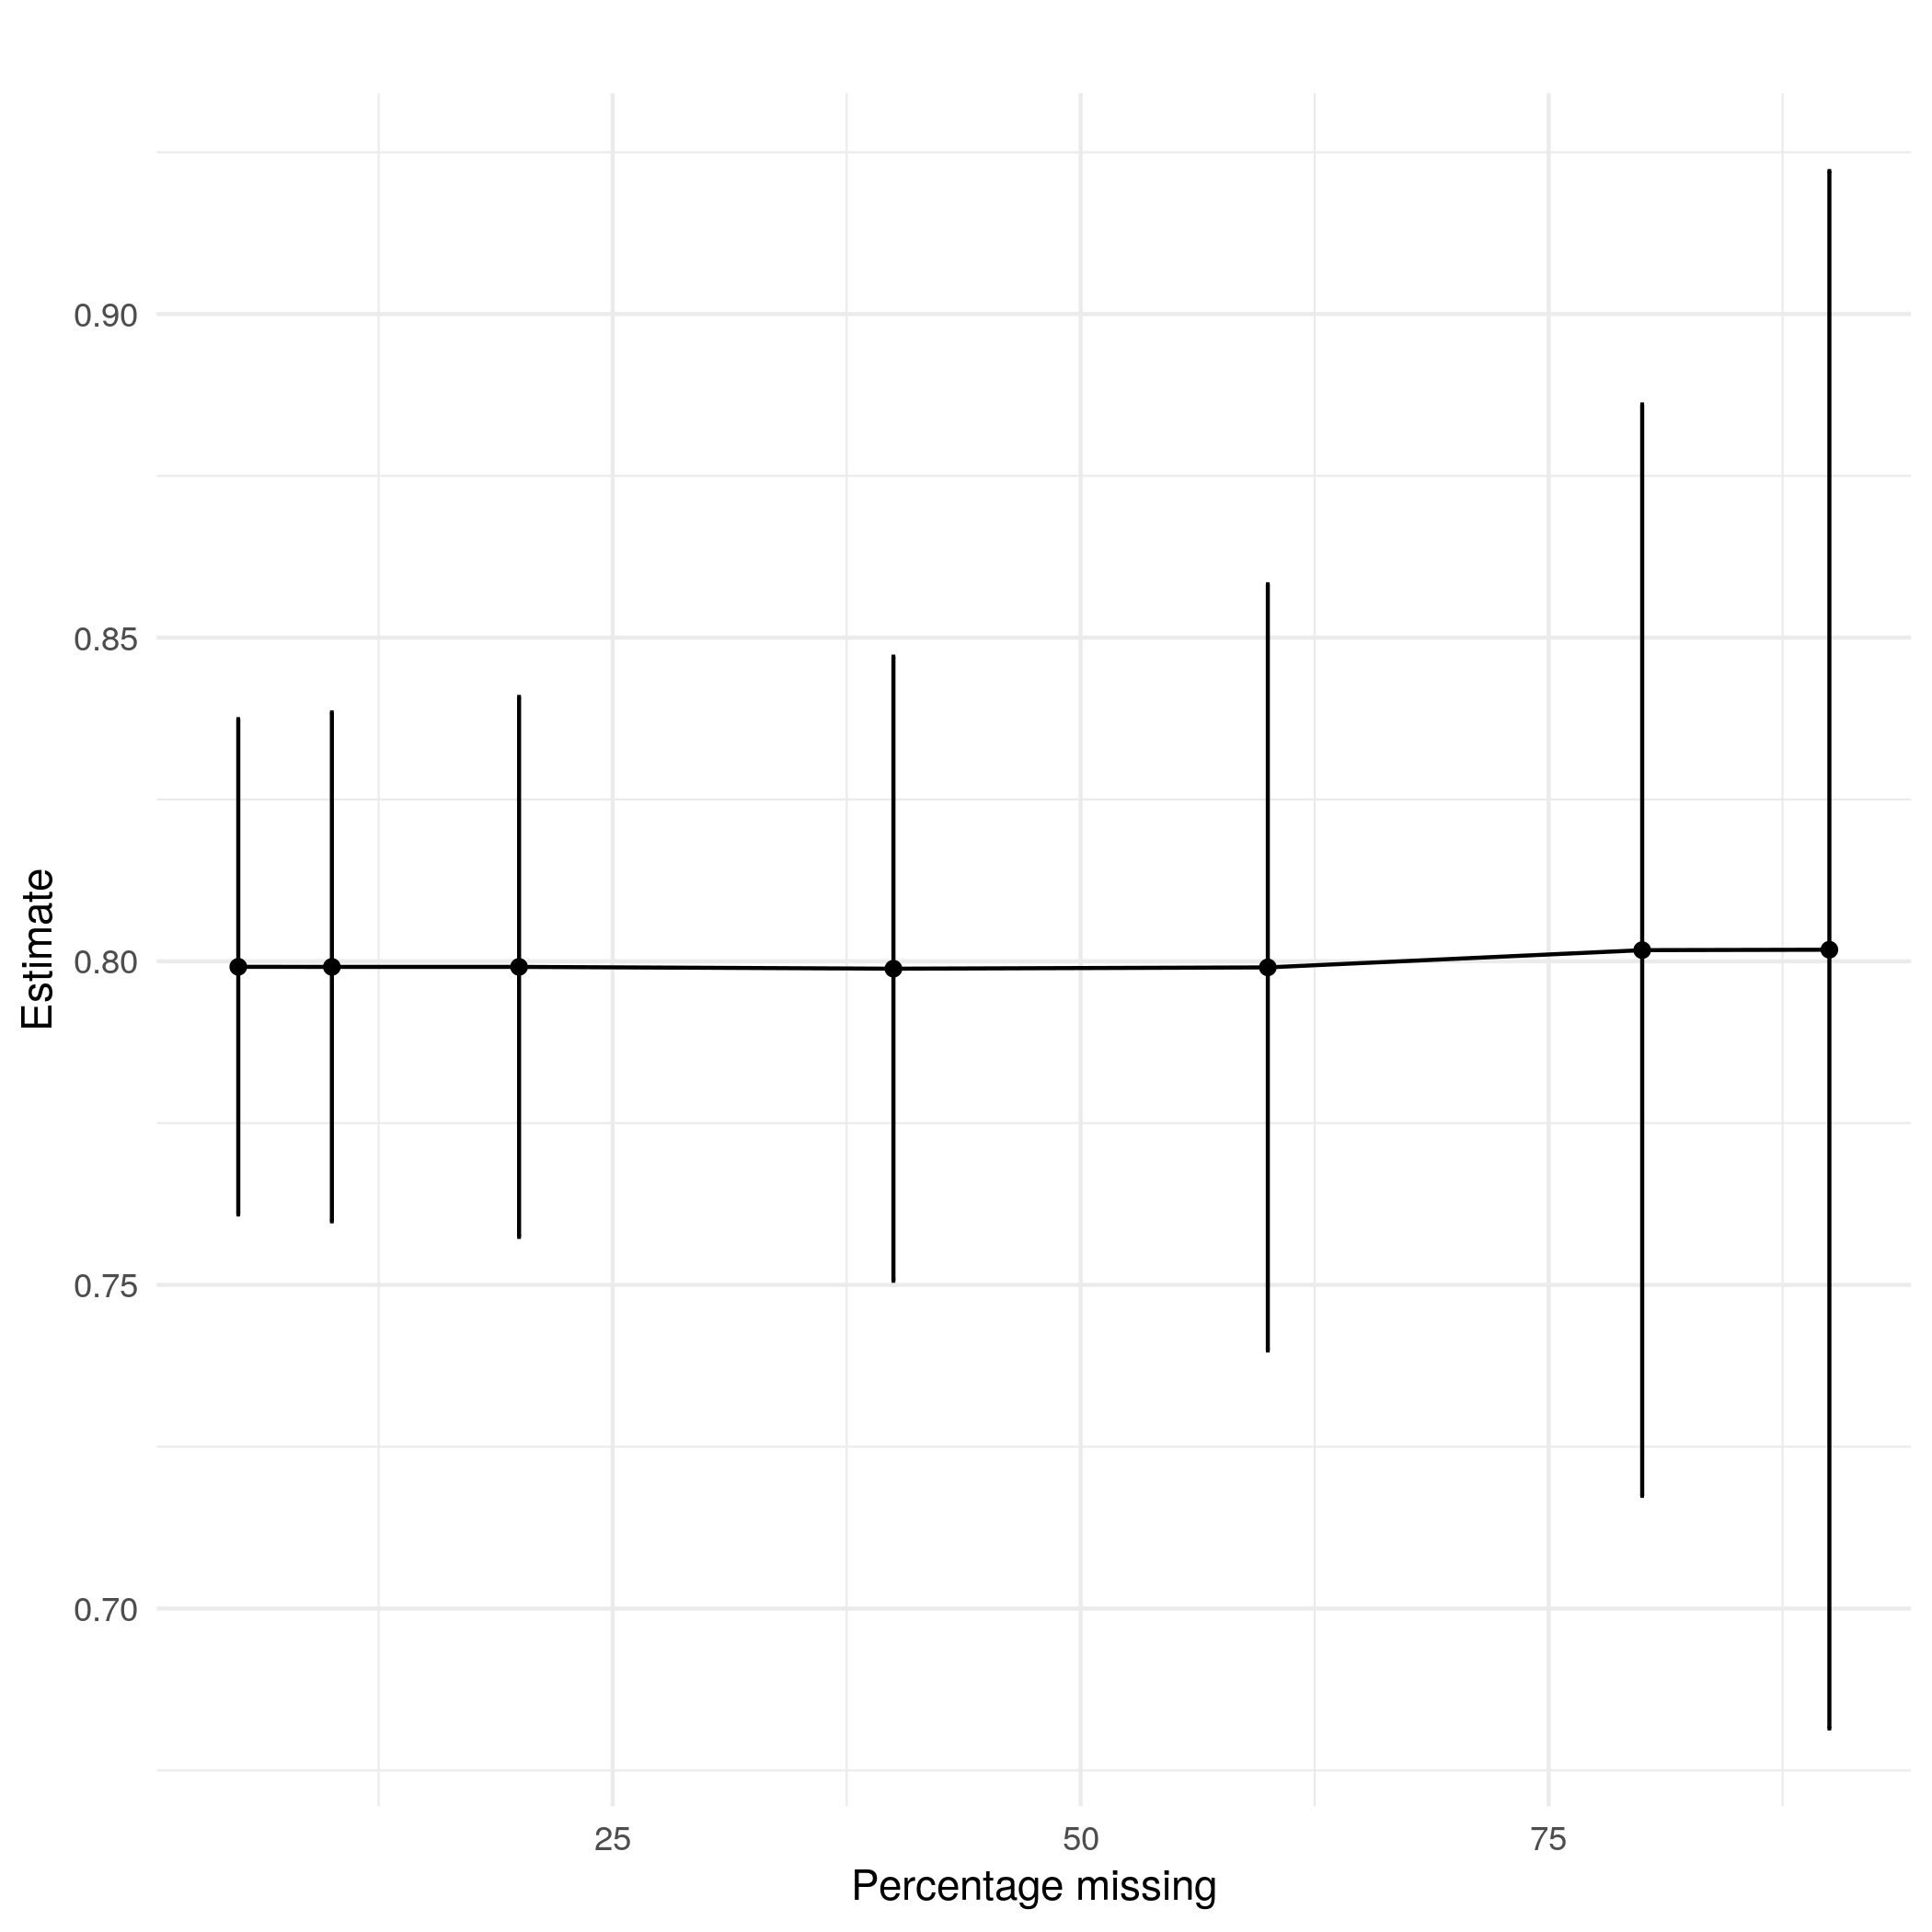
\includegraphics[width=0.3\textwidth]{mcar_estimate_cca.png}}
	\quad
	\subfloat[$\beta_{1}$ estimate with MI]{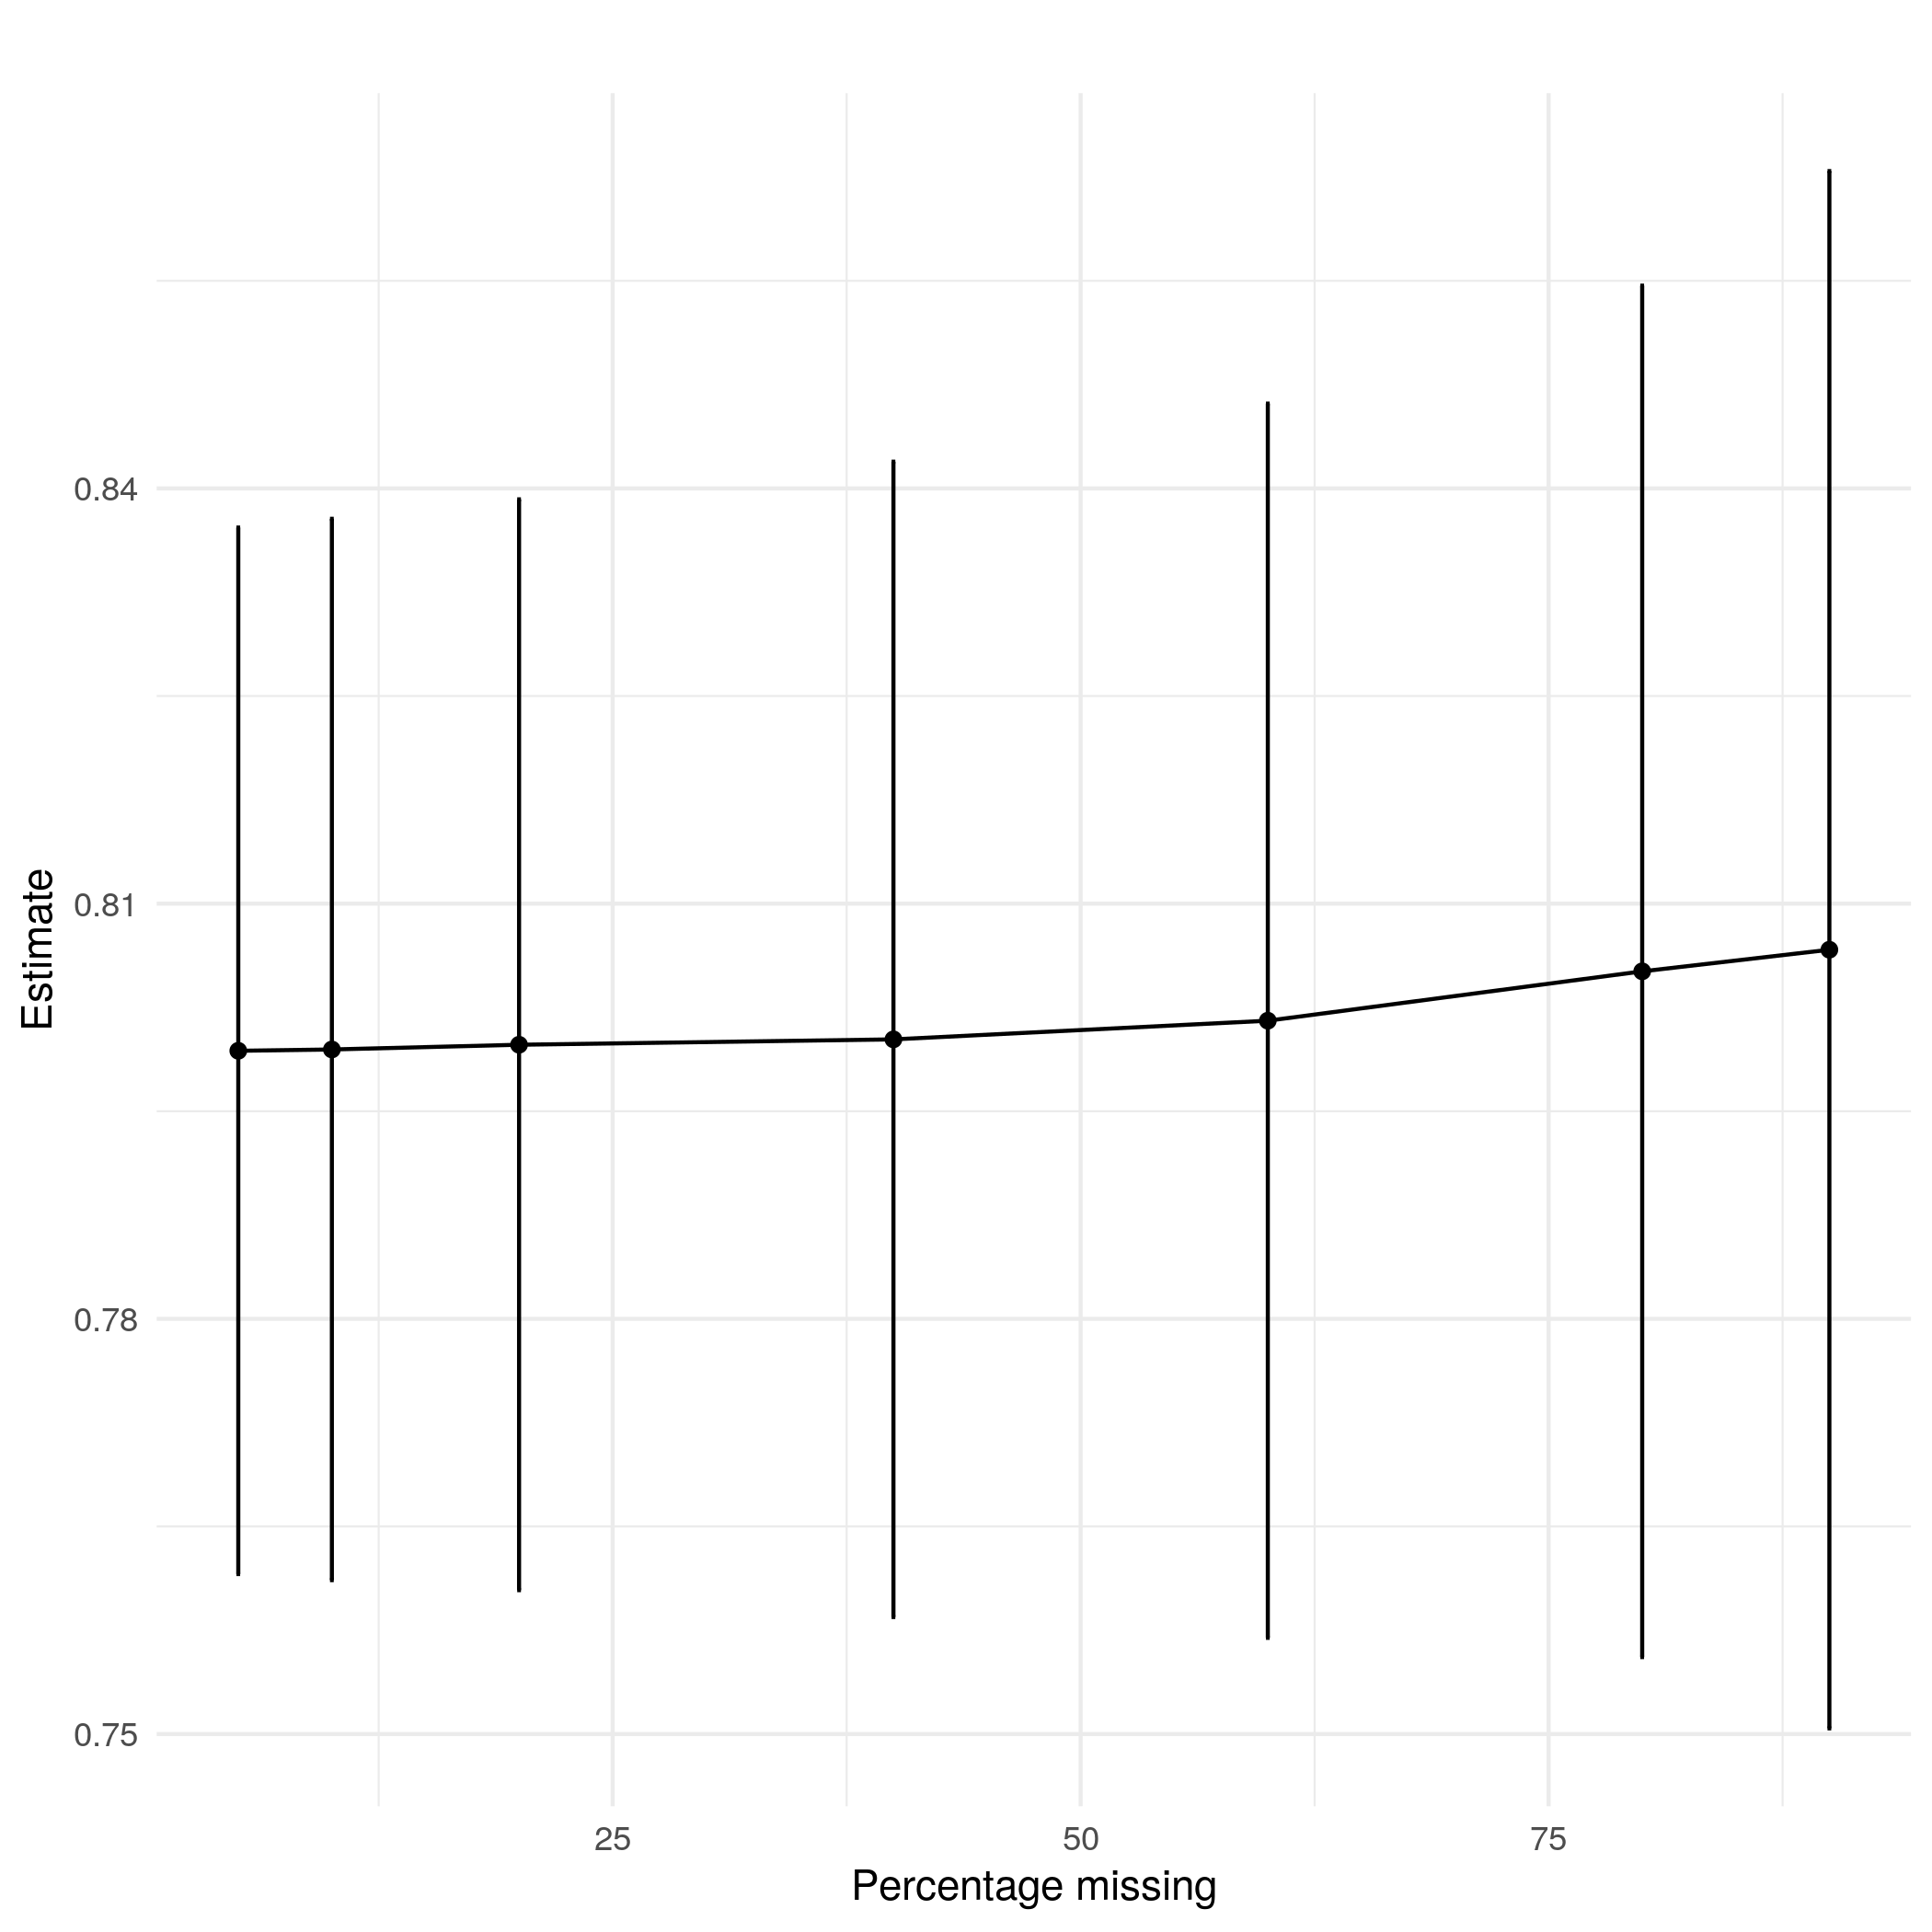
\includegraphics[width=0.3\textwidth]{mcar_estimate_mi.png}}
	\\
	\subfloat[Coverage]{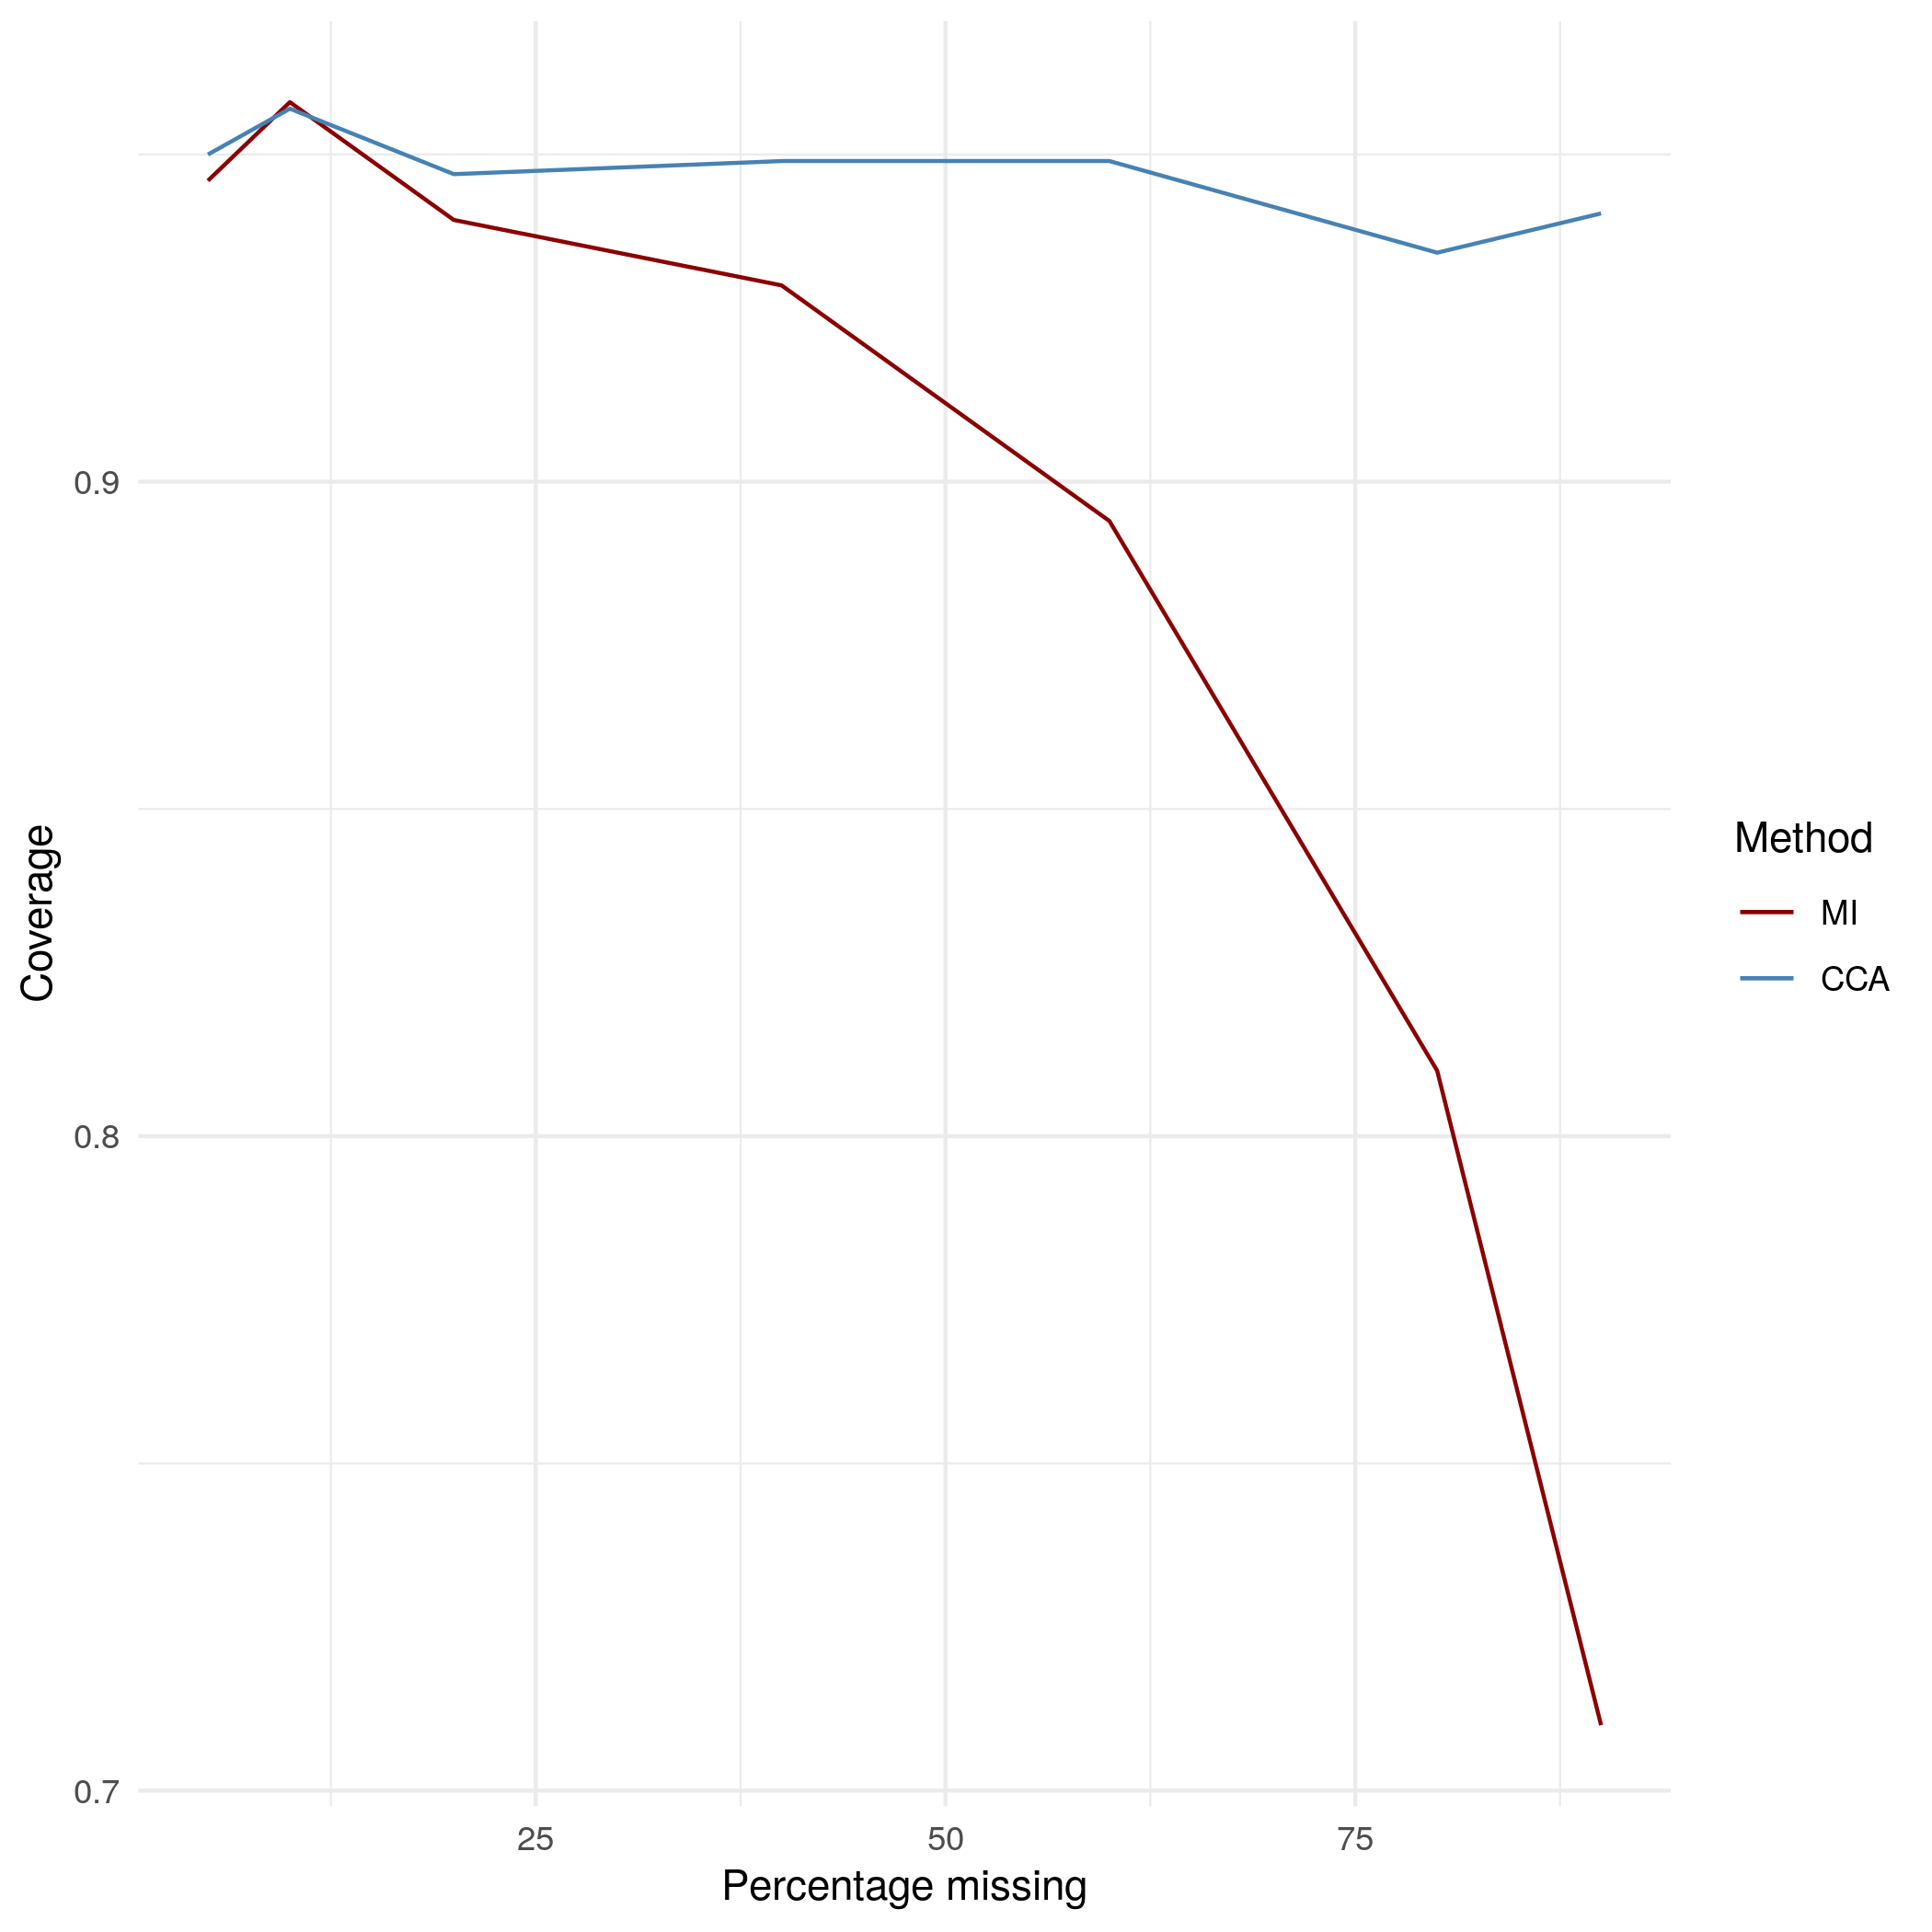
\includegraphics[width=0.2\textwidth]{mcar_coverage.png}}
	\quad
	\subfloat[Average CI size]{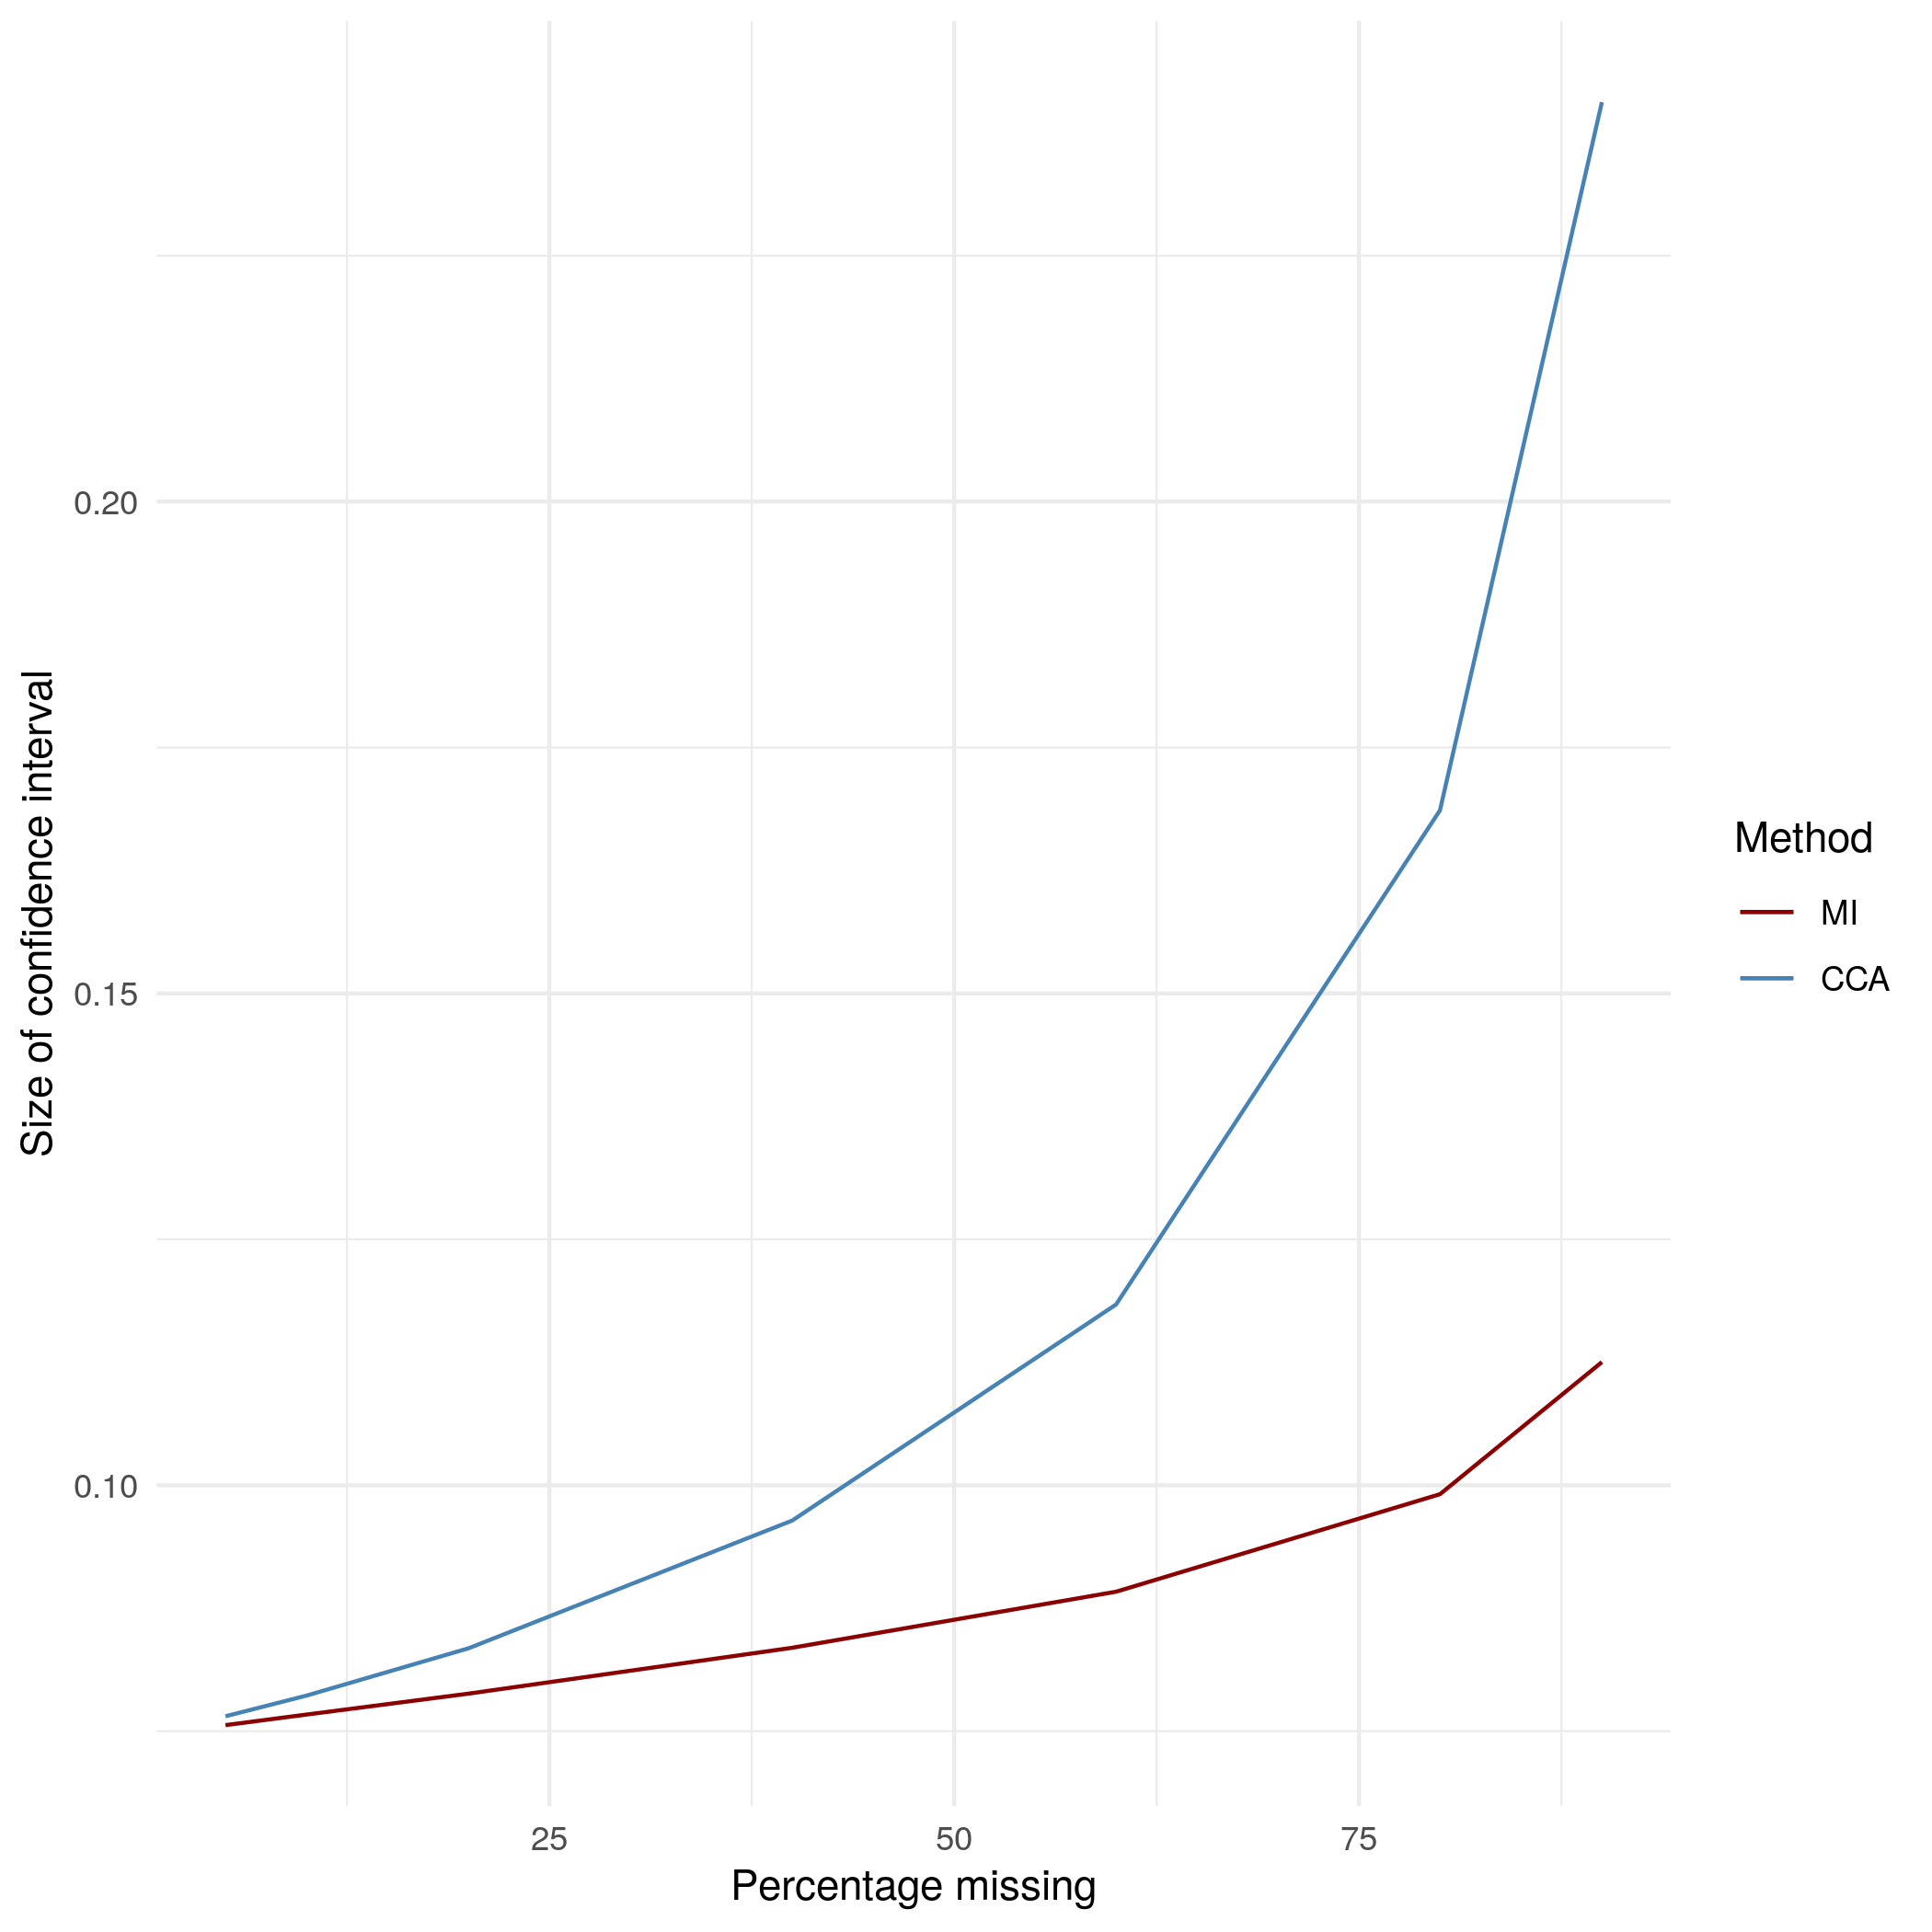
\includegraphics[width=0.2\textwidth]{mcar_ci.png}}
	\quad
	\subfloat[Average bias]{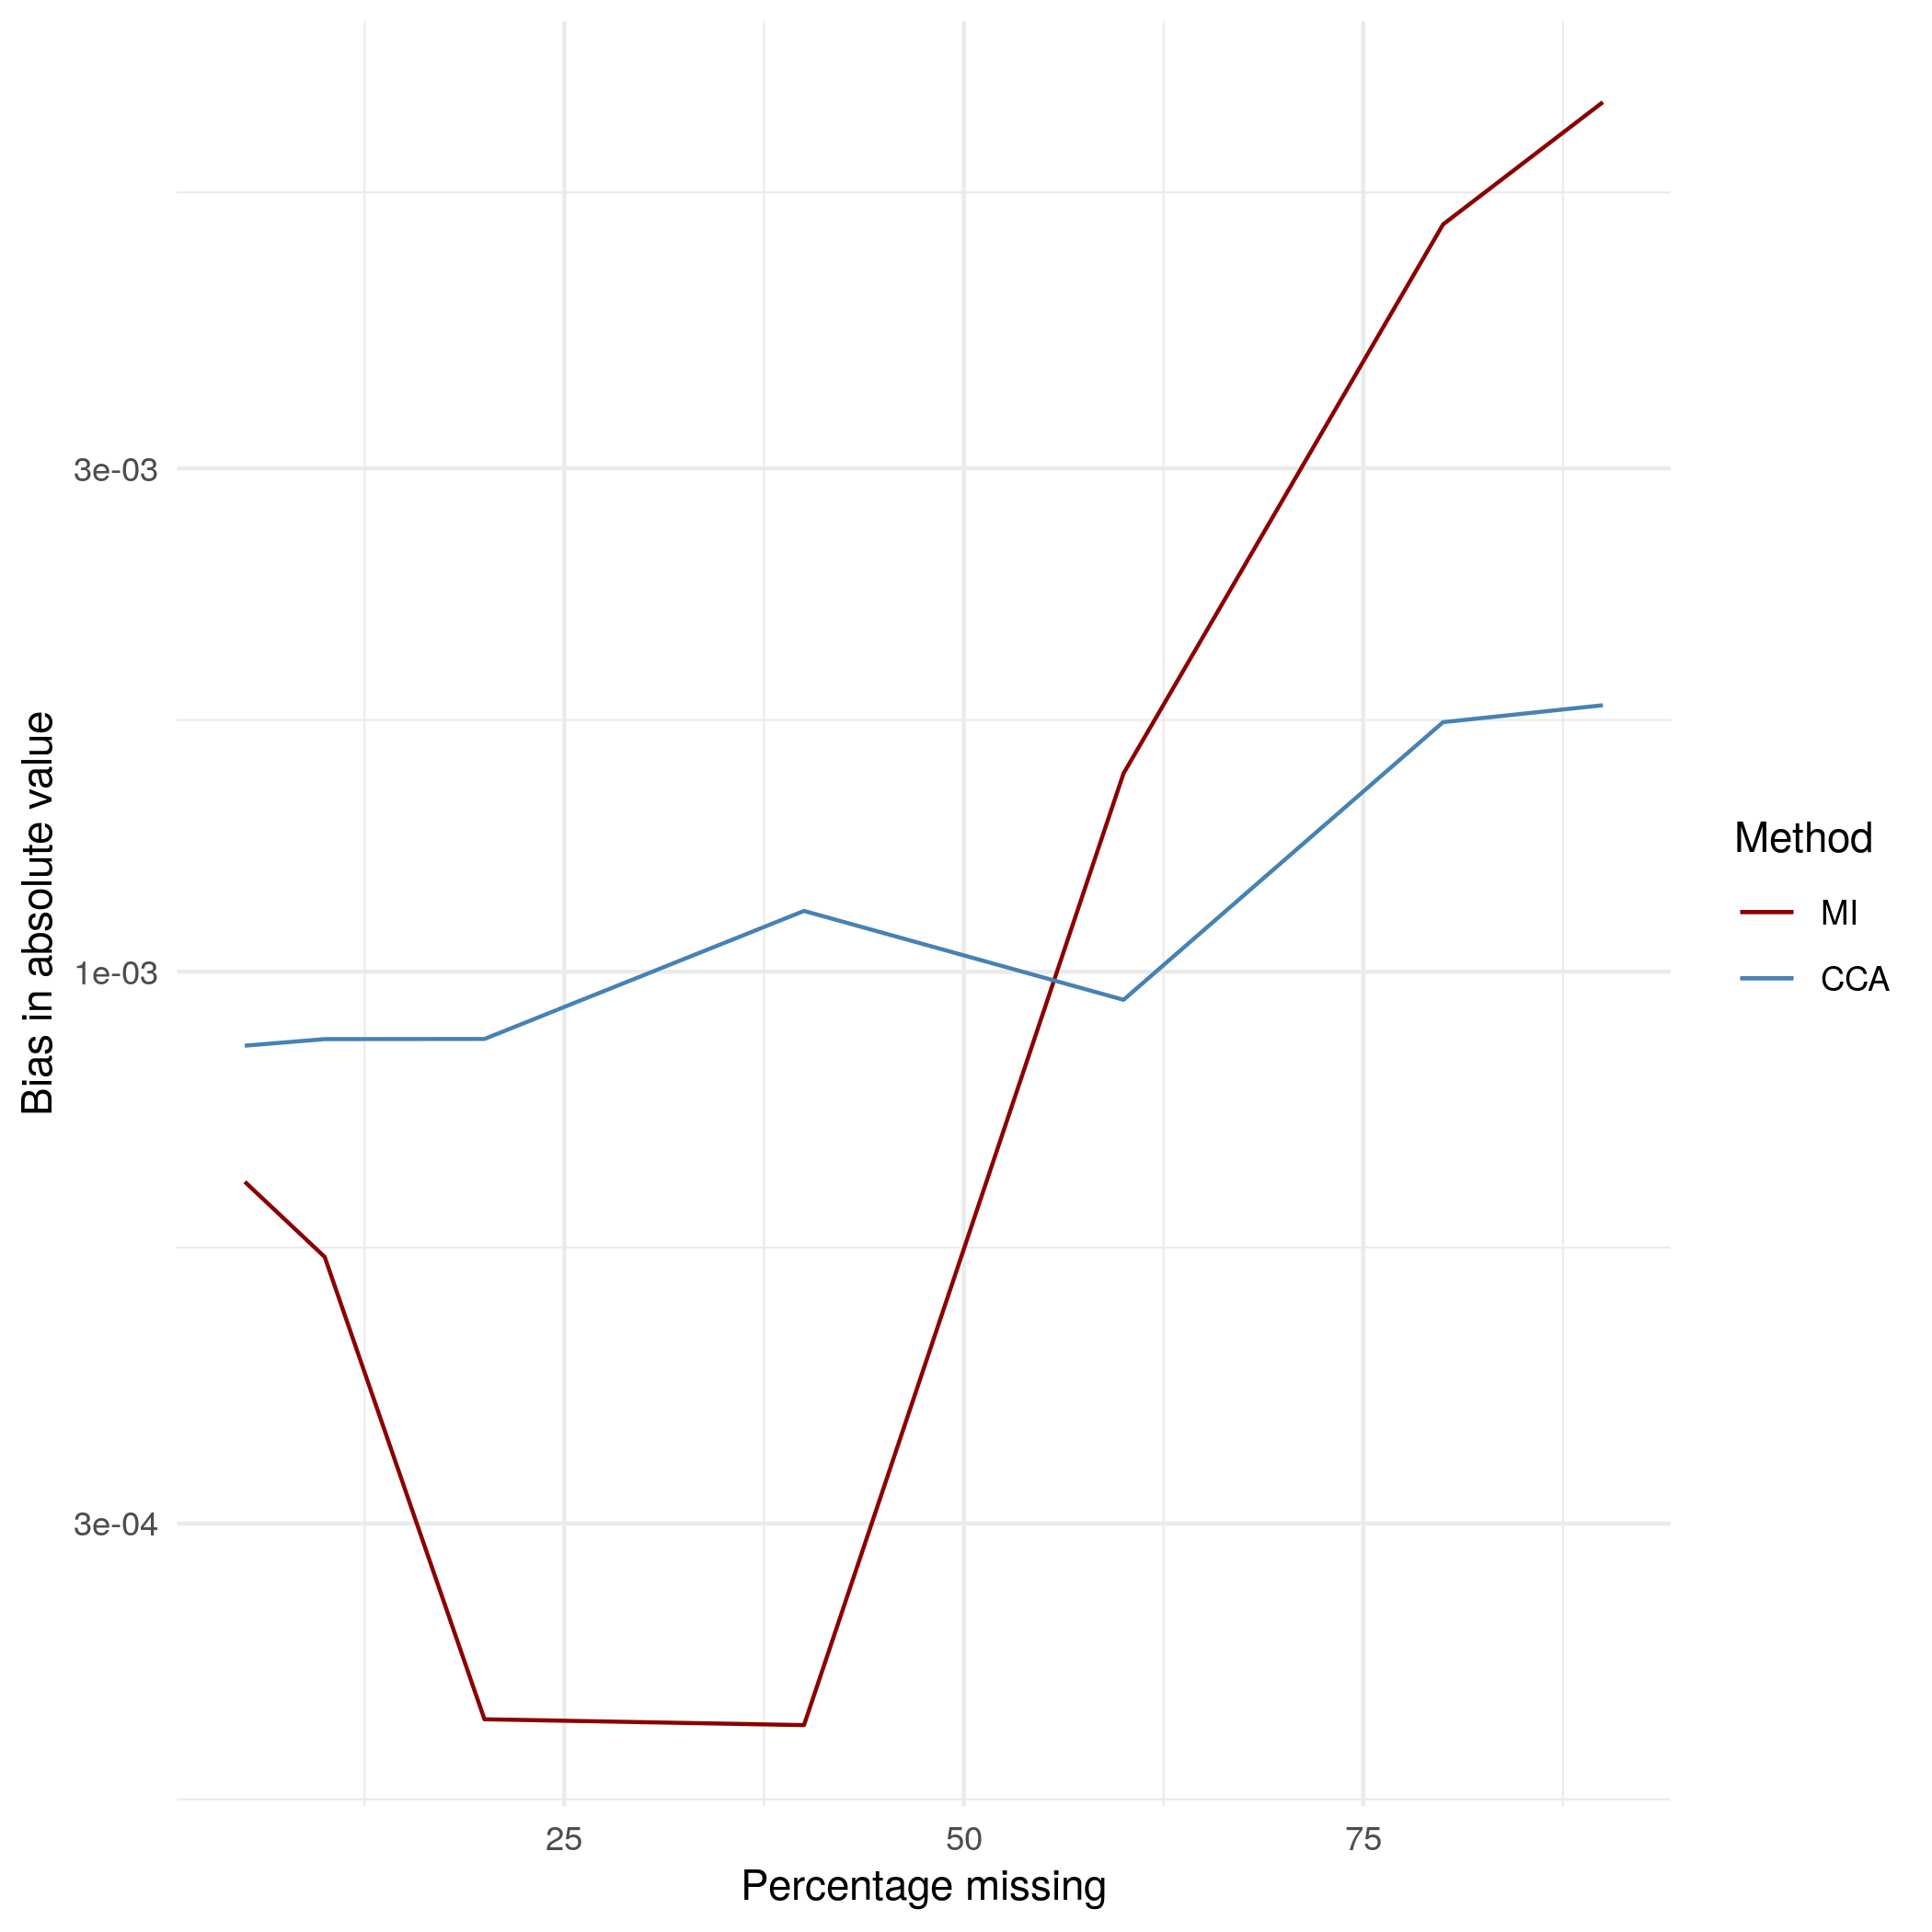
\includegraphics[width=0.2\textwidth]{mcar_bias.png}}
\end{figure}
\end{frame}

\begin{frame}
\frametitle{MAR in X}
\begin{figure}[H]
	\centering
	\subfloat[$\beta_{1}$ estimate with CCA]{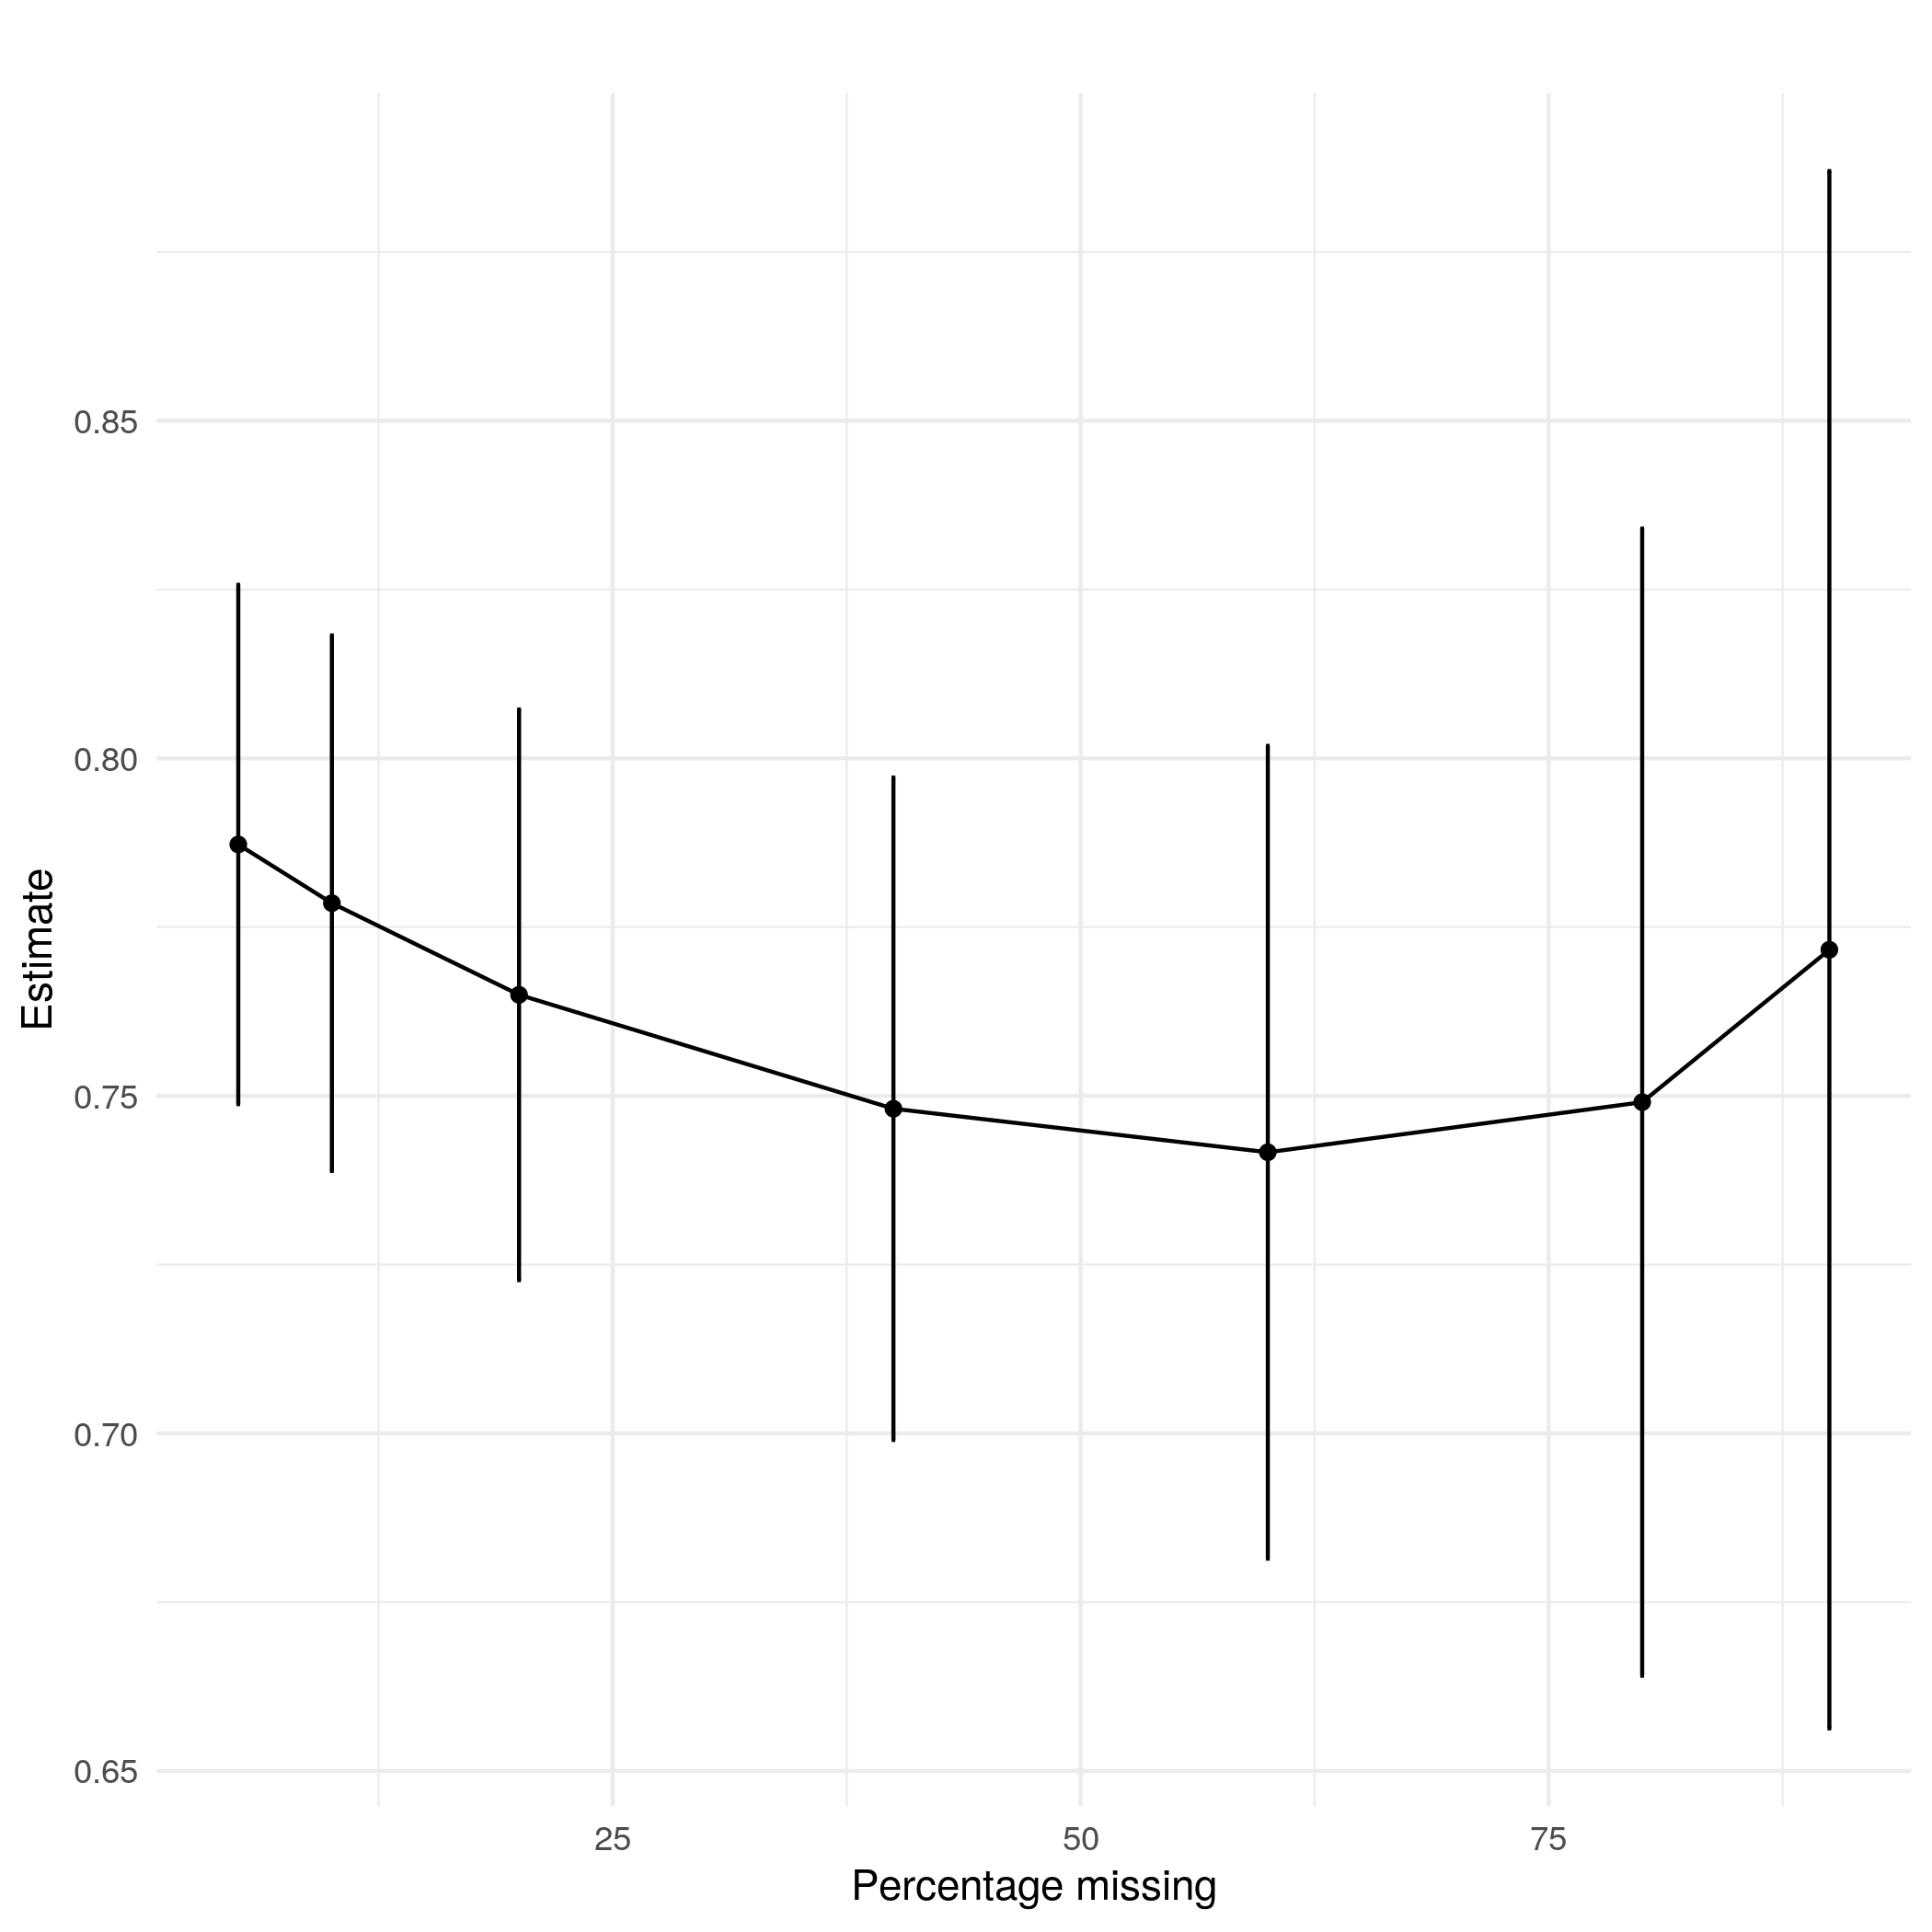
\includegraphics[width=0.3\textwidth]{mar_reg_x_estimate_cca.png}}
	\quad
	\subfloat[$\beta_{1}$ estimate with MI]{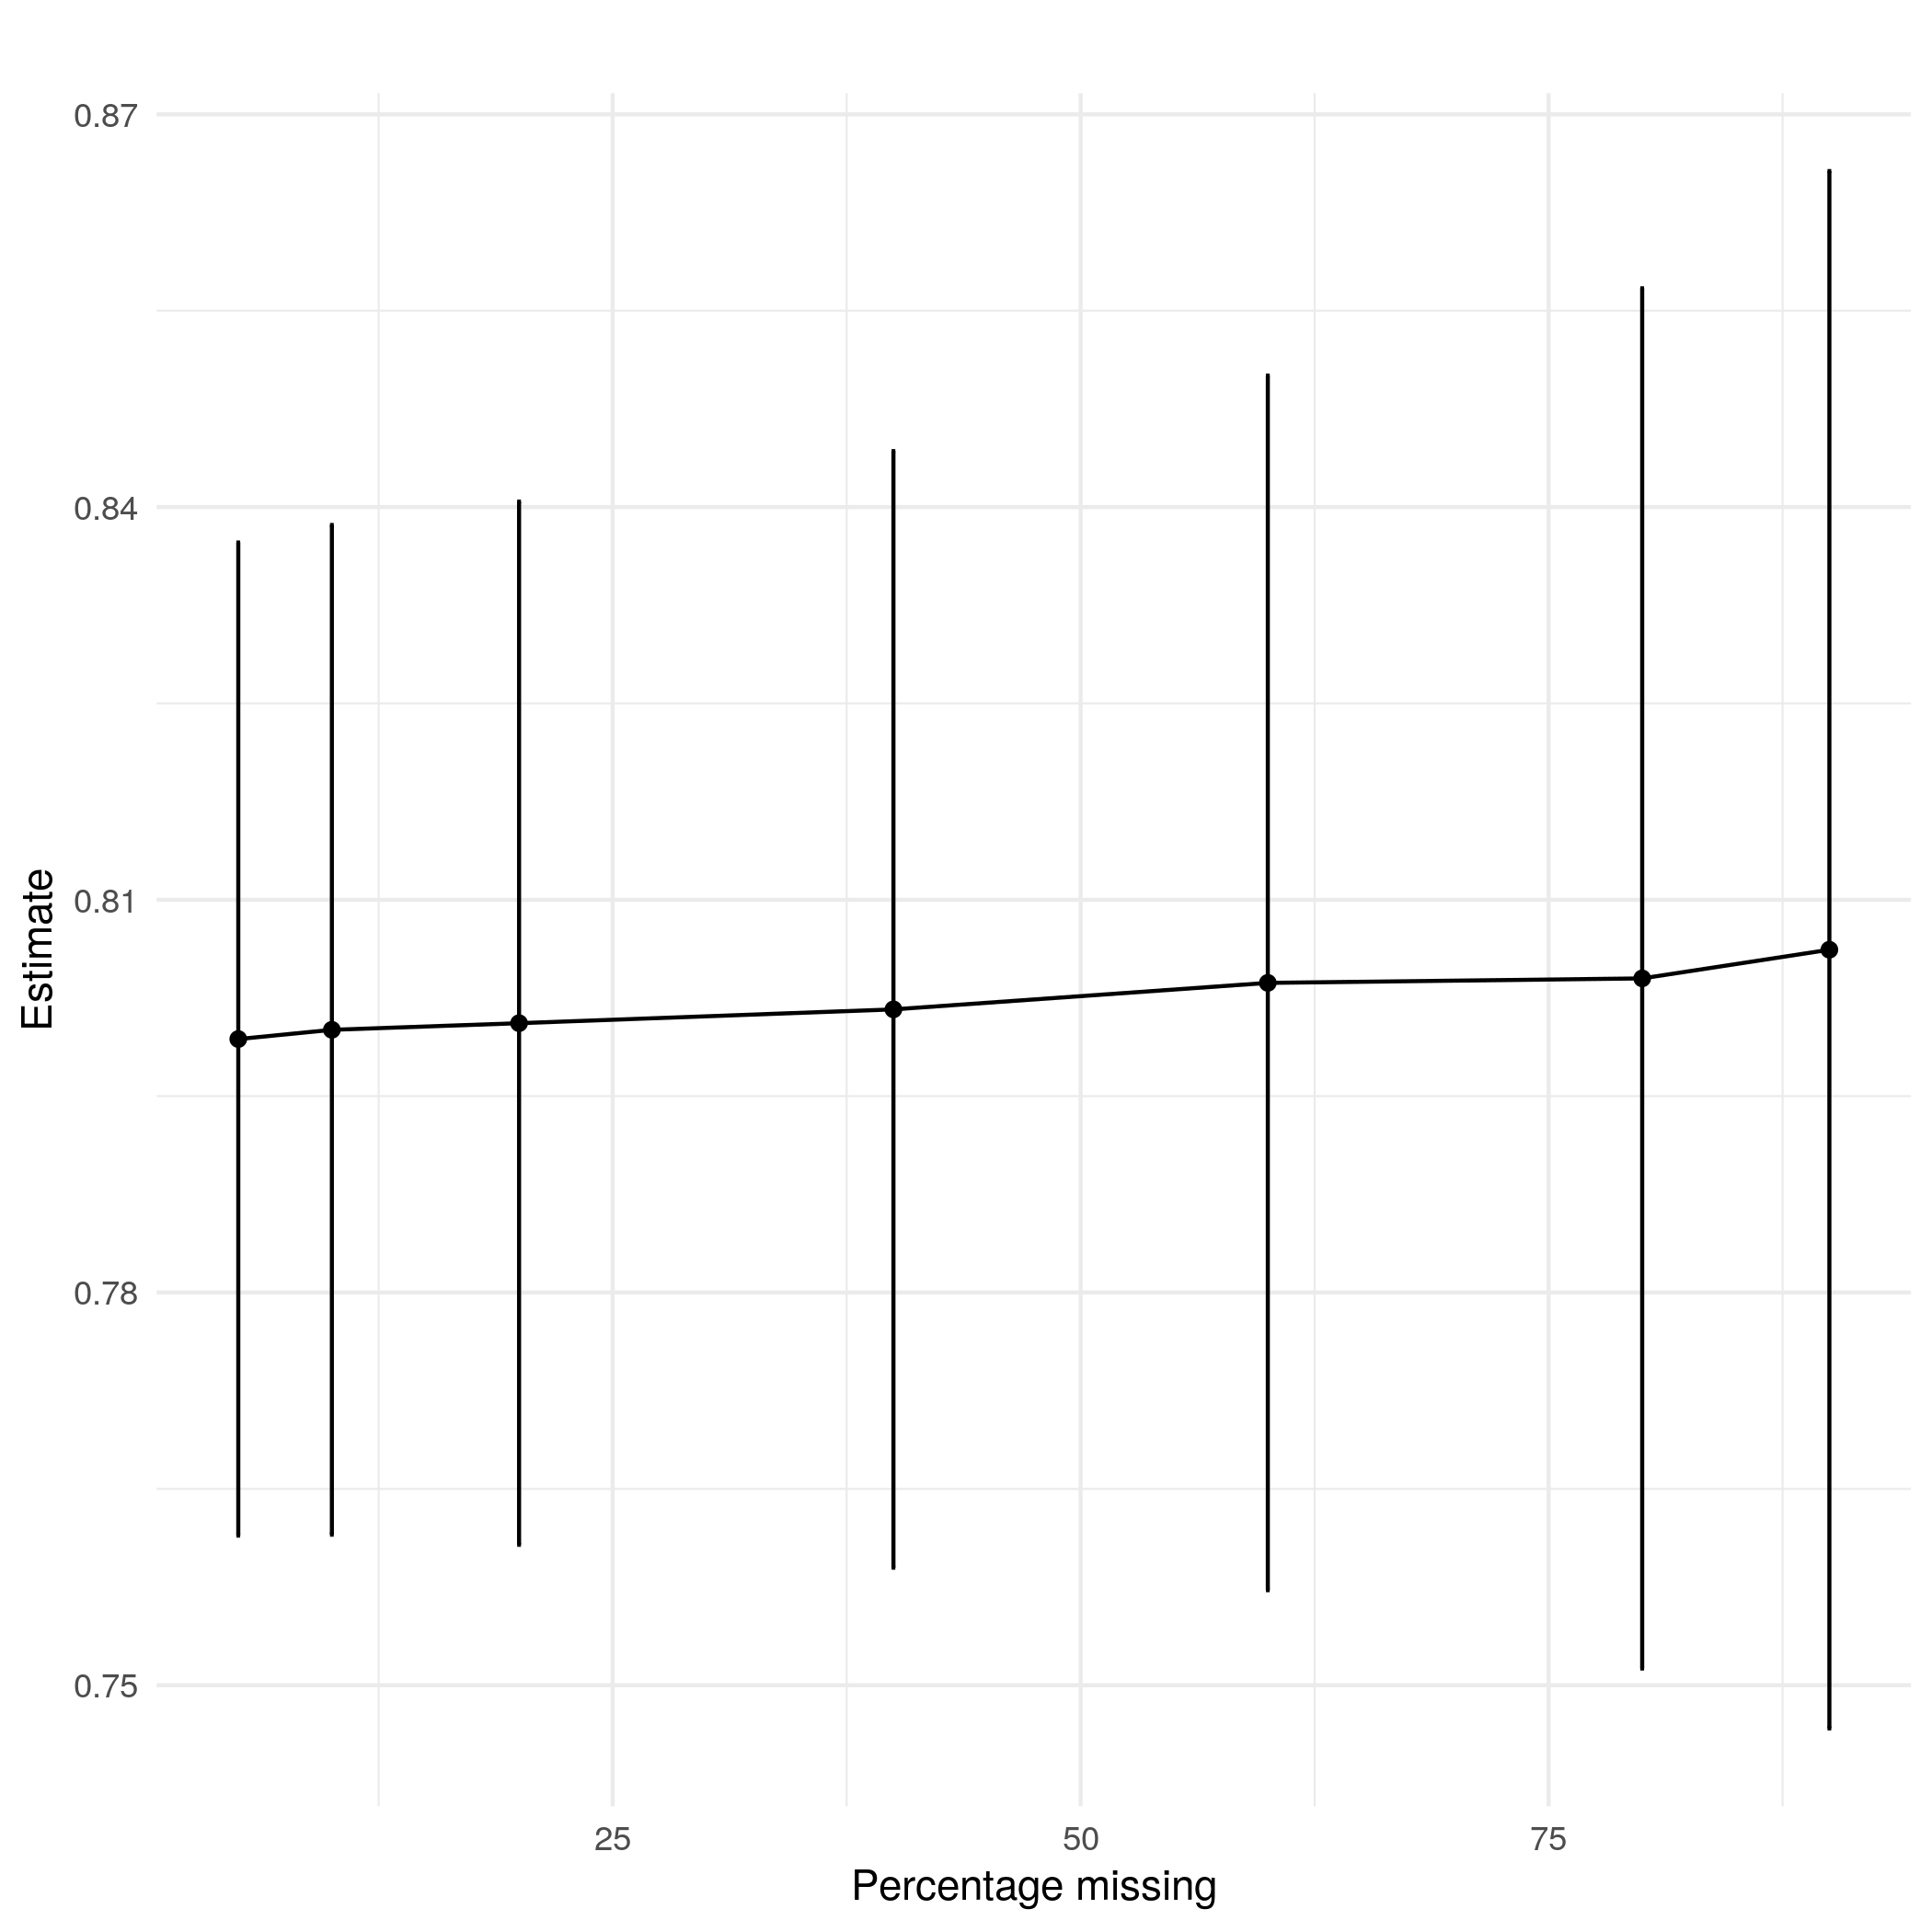
\includegraphics[width=0.3\textwidth]{mar_reg_x_estimate_mi.png}}
	\\
	\subfloat[Coverage]{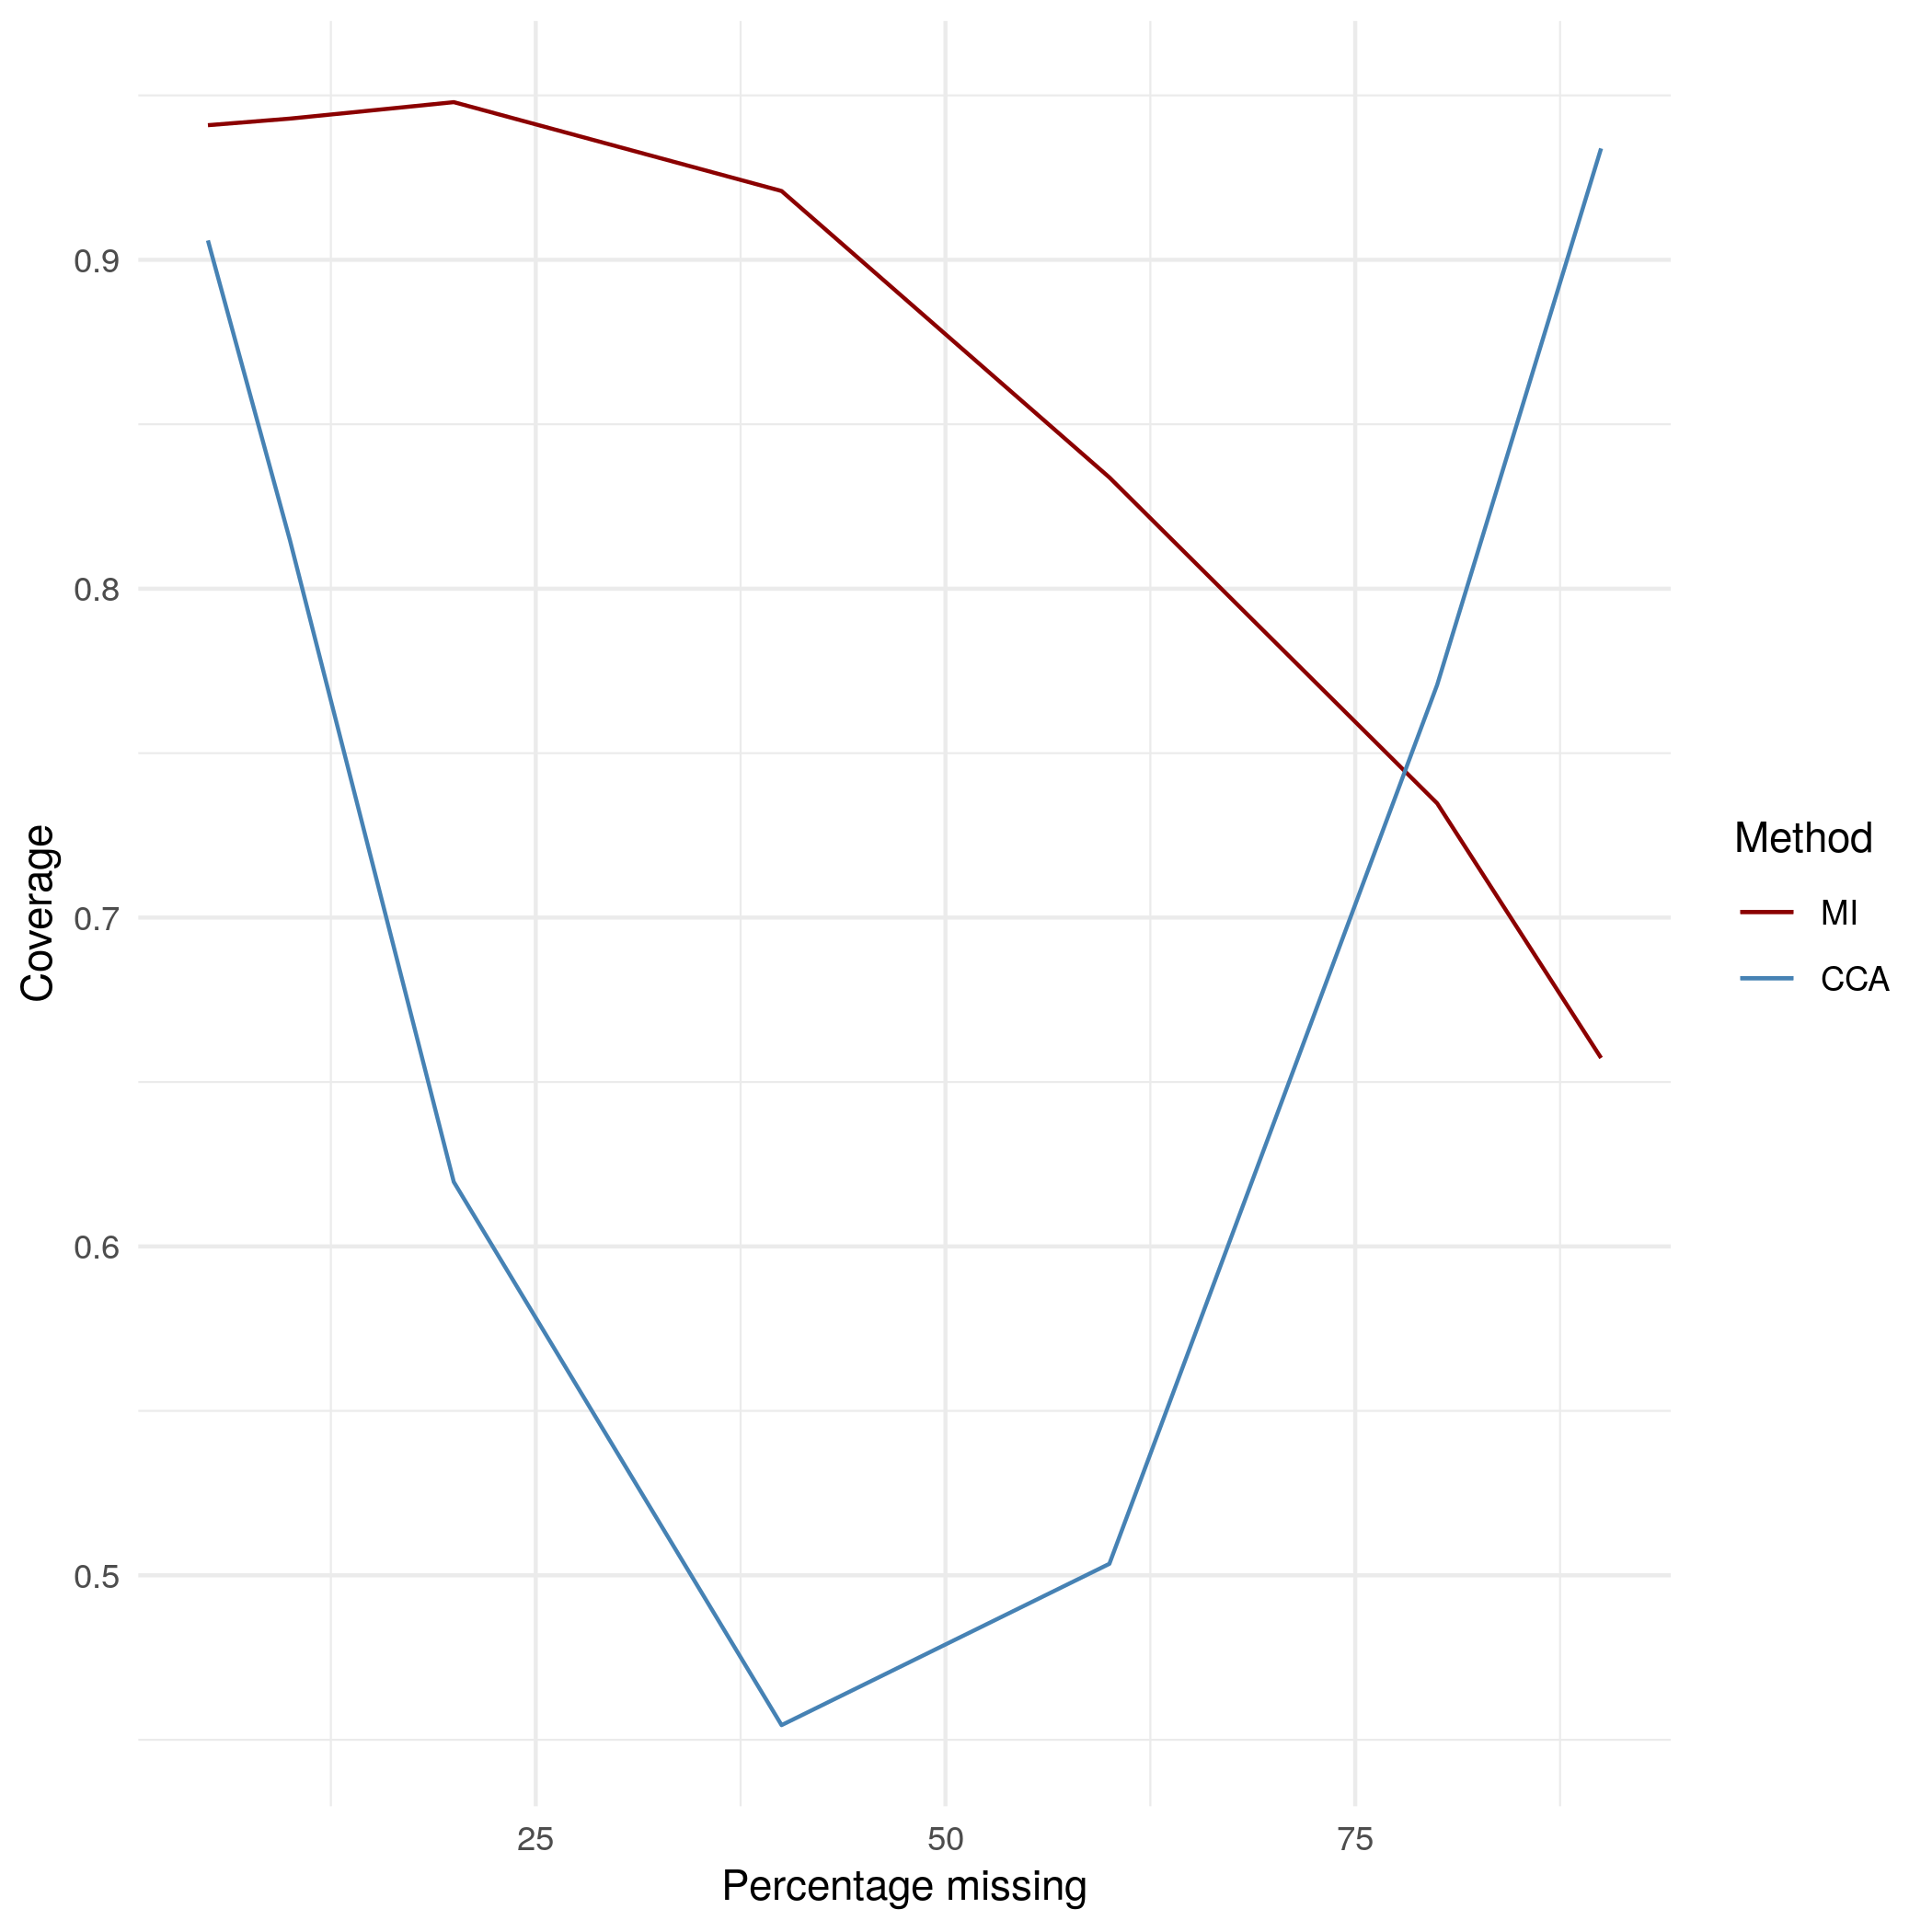
\includegraphics[width=0.2\textwidth]{mar_reg_x_coverage.png}}
	\quad
	\subfloat[Average CI size]{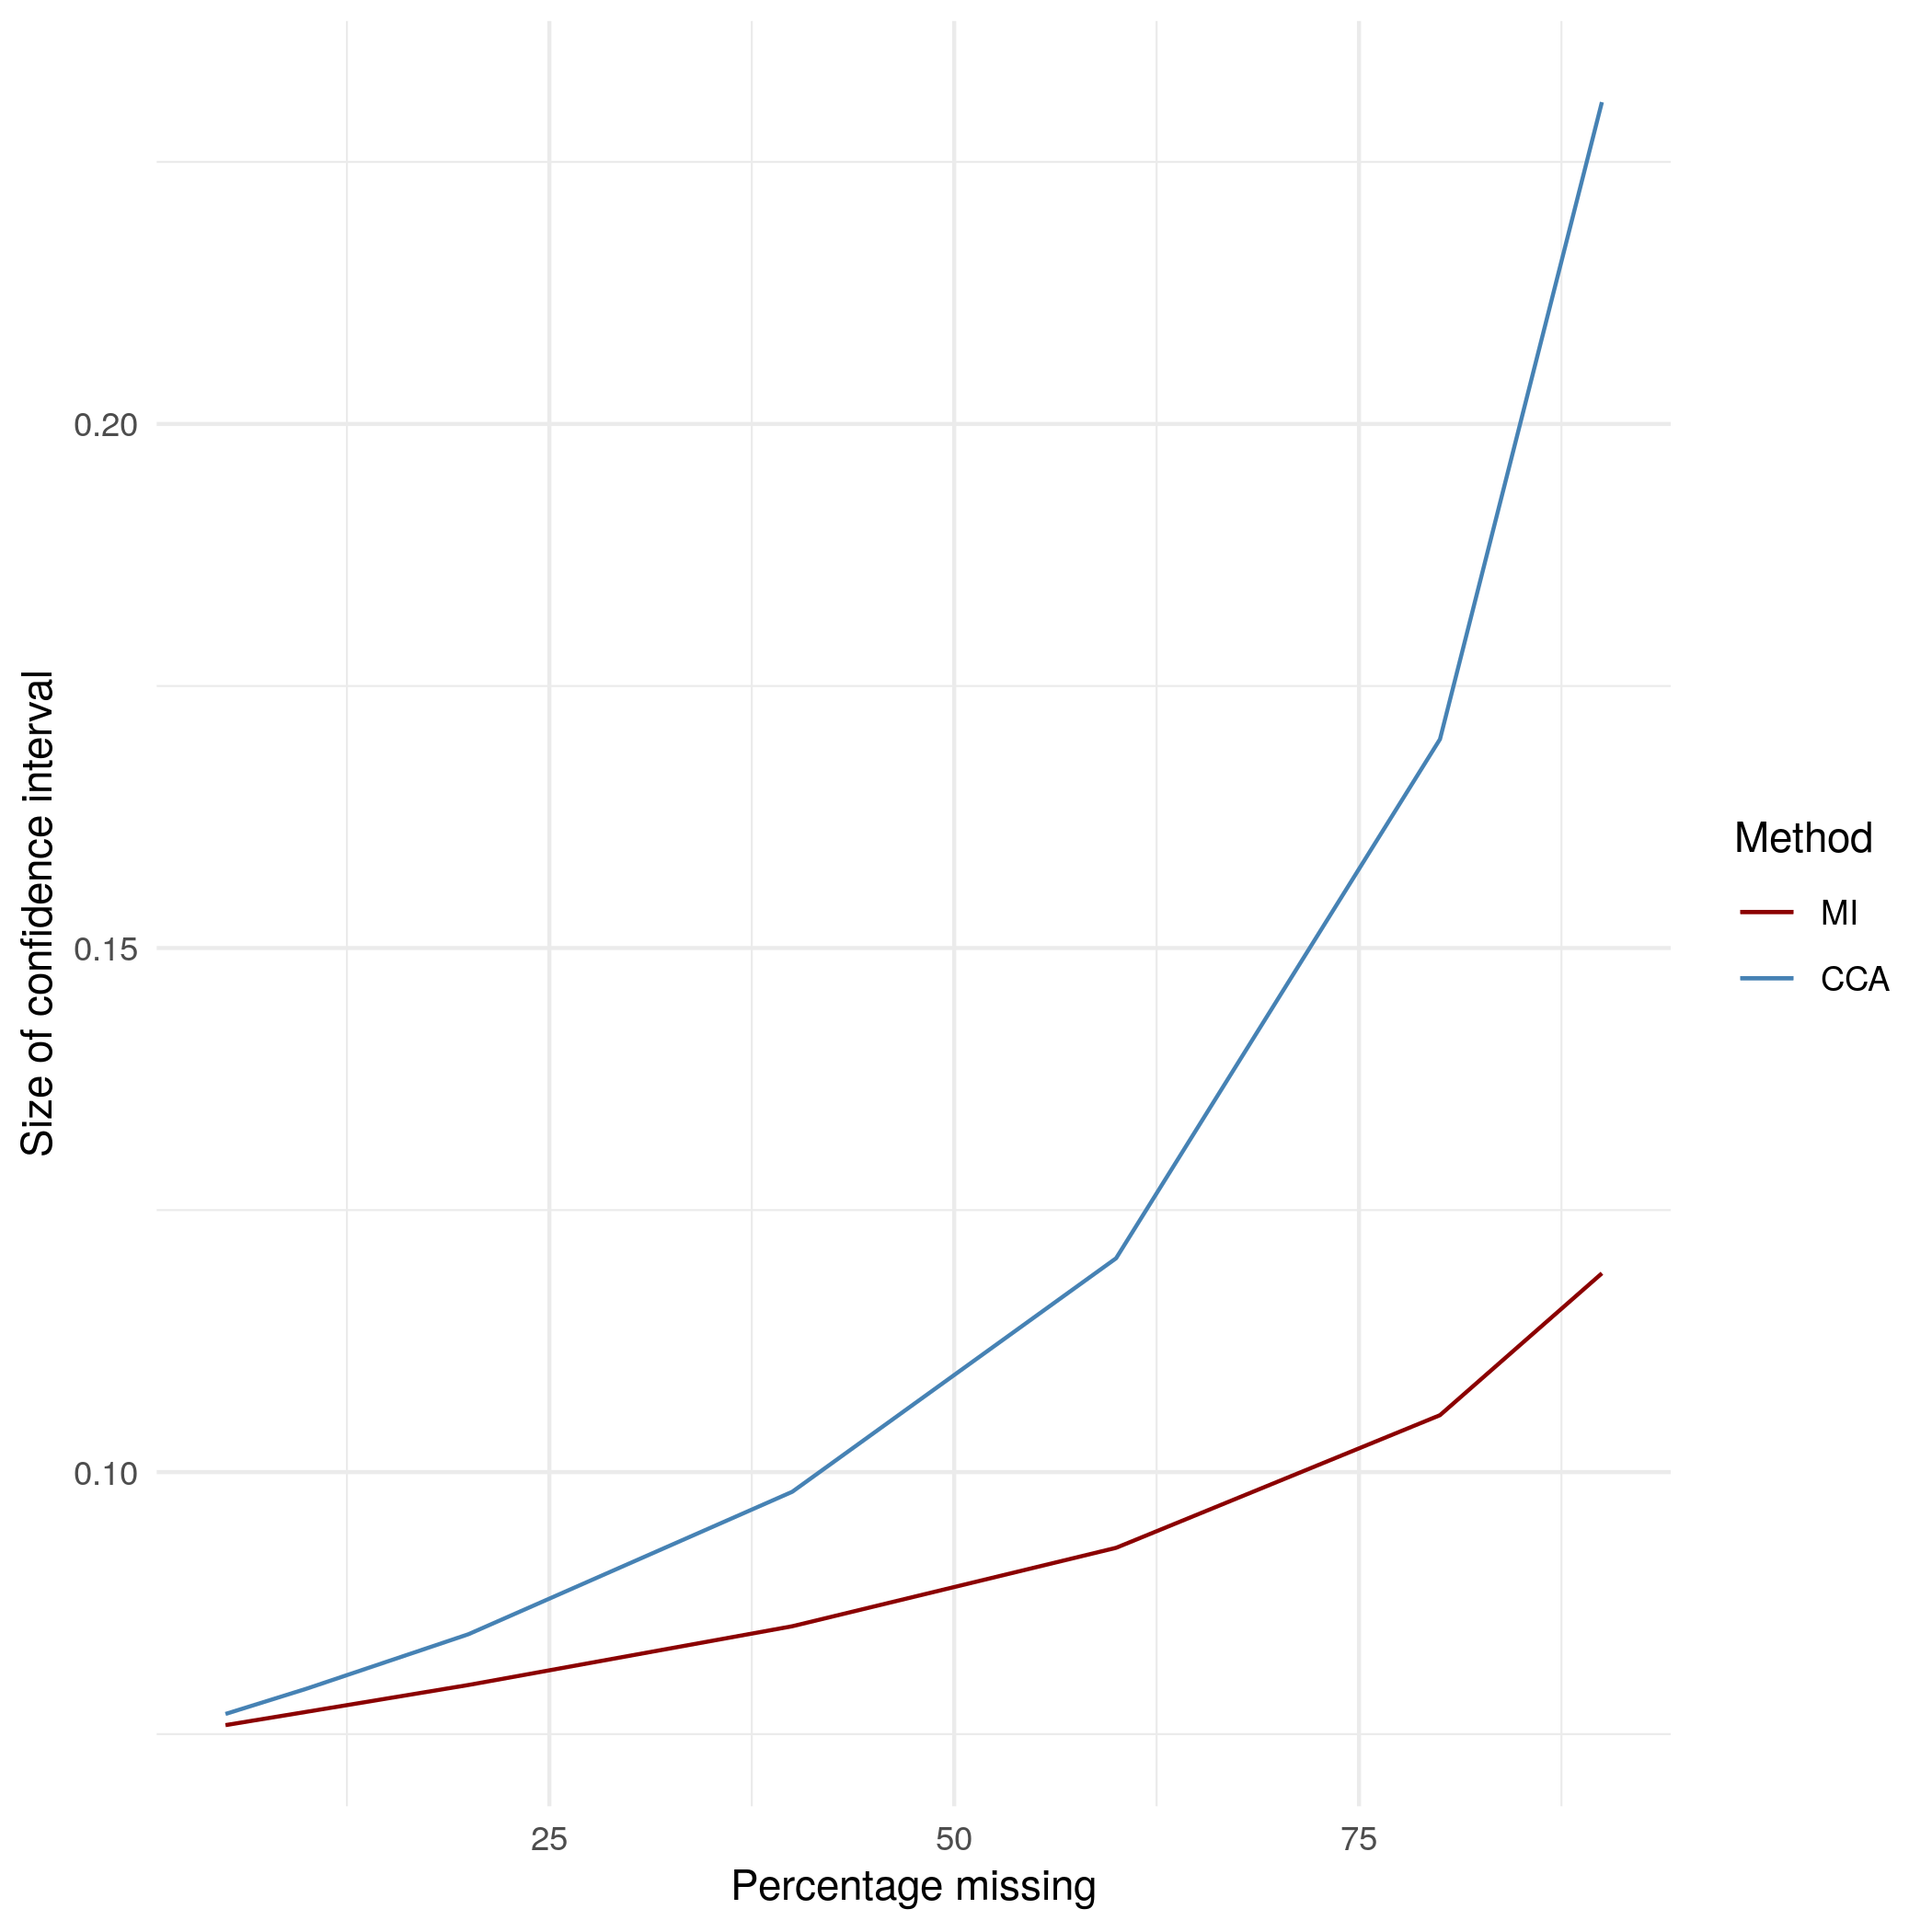
\includegraphics[width=0.2\textwidth]{mar_reg_x_ci.png}}
	\quad
	\subfloat[Average bias]{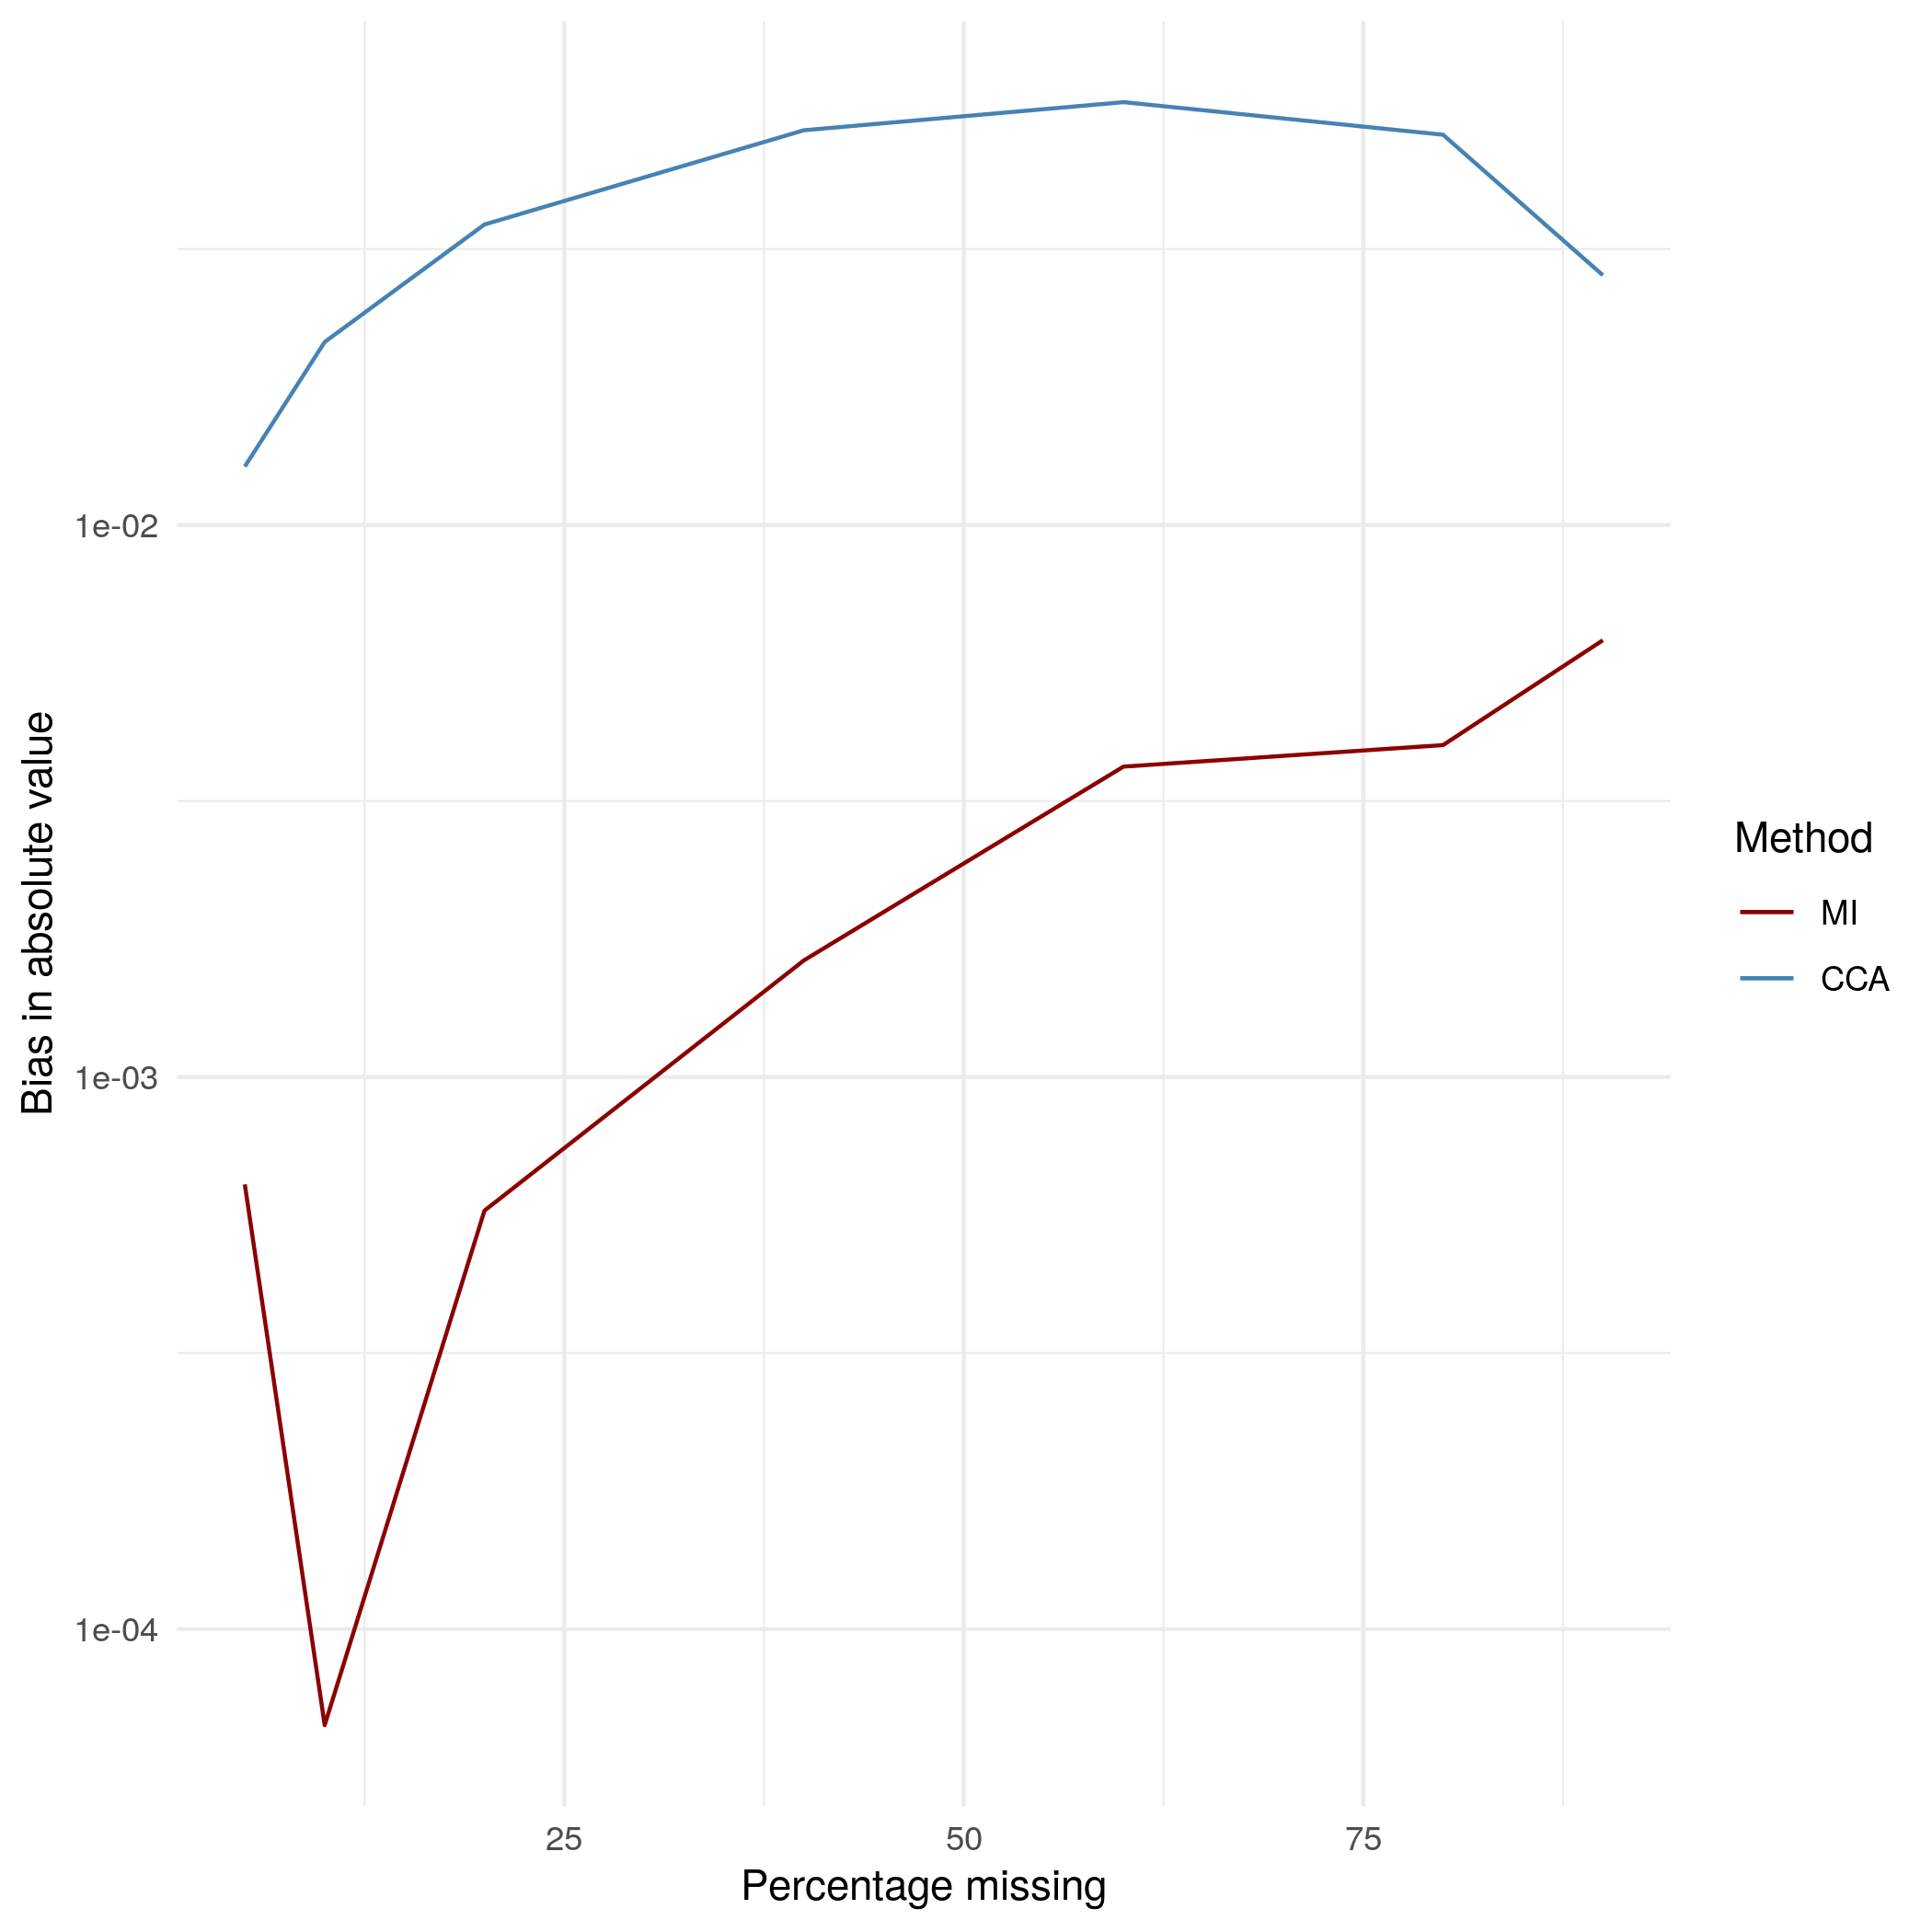
\includegraphics[width=0.2\textwidth]{mar_reg_x_bias.png}}
\end{figure}
\end{frame}

\begin{frame}
\frametitle{MAR in Y}
\begin{figure}[H]
	\centering
	\subfloat[$\beta_{1}$ estimate with CCA]{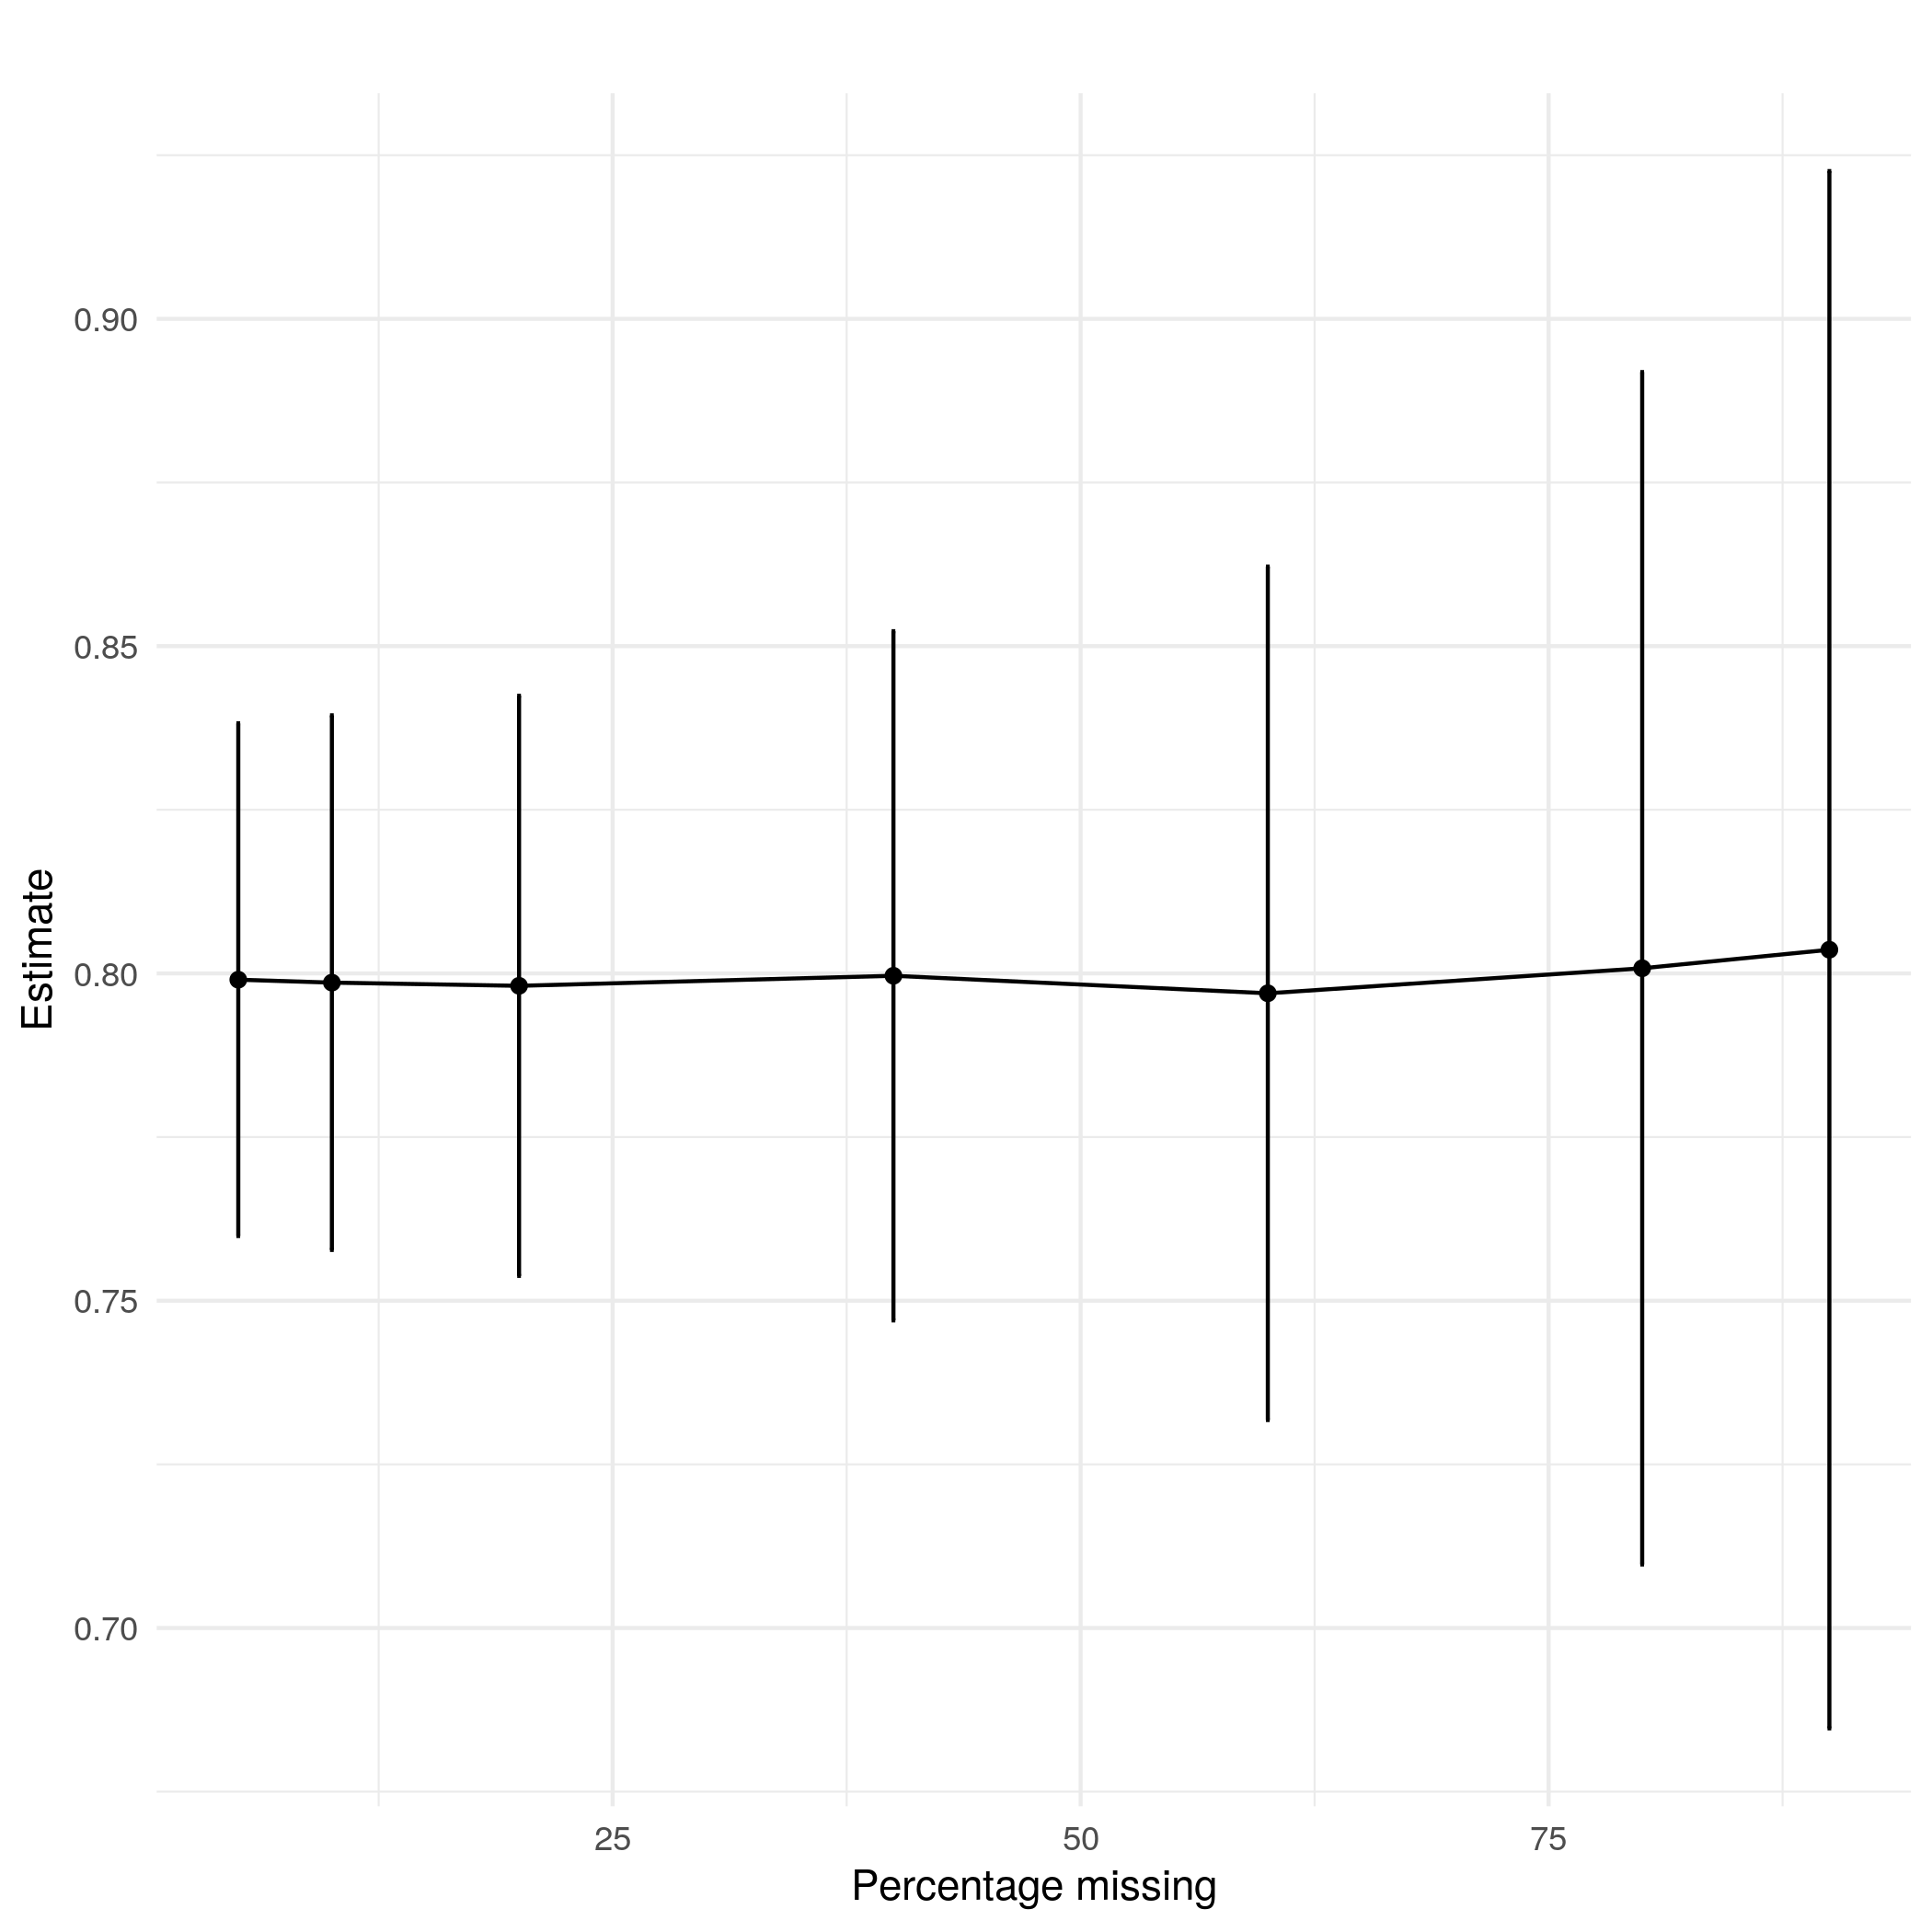
\includegraphics[width=0.3\textwidth]{final_estimate_cca.png}}
	\quad
	\subfloat[$\beta_{1}$ estimate with MI]{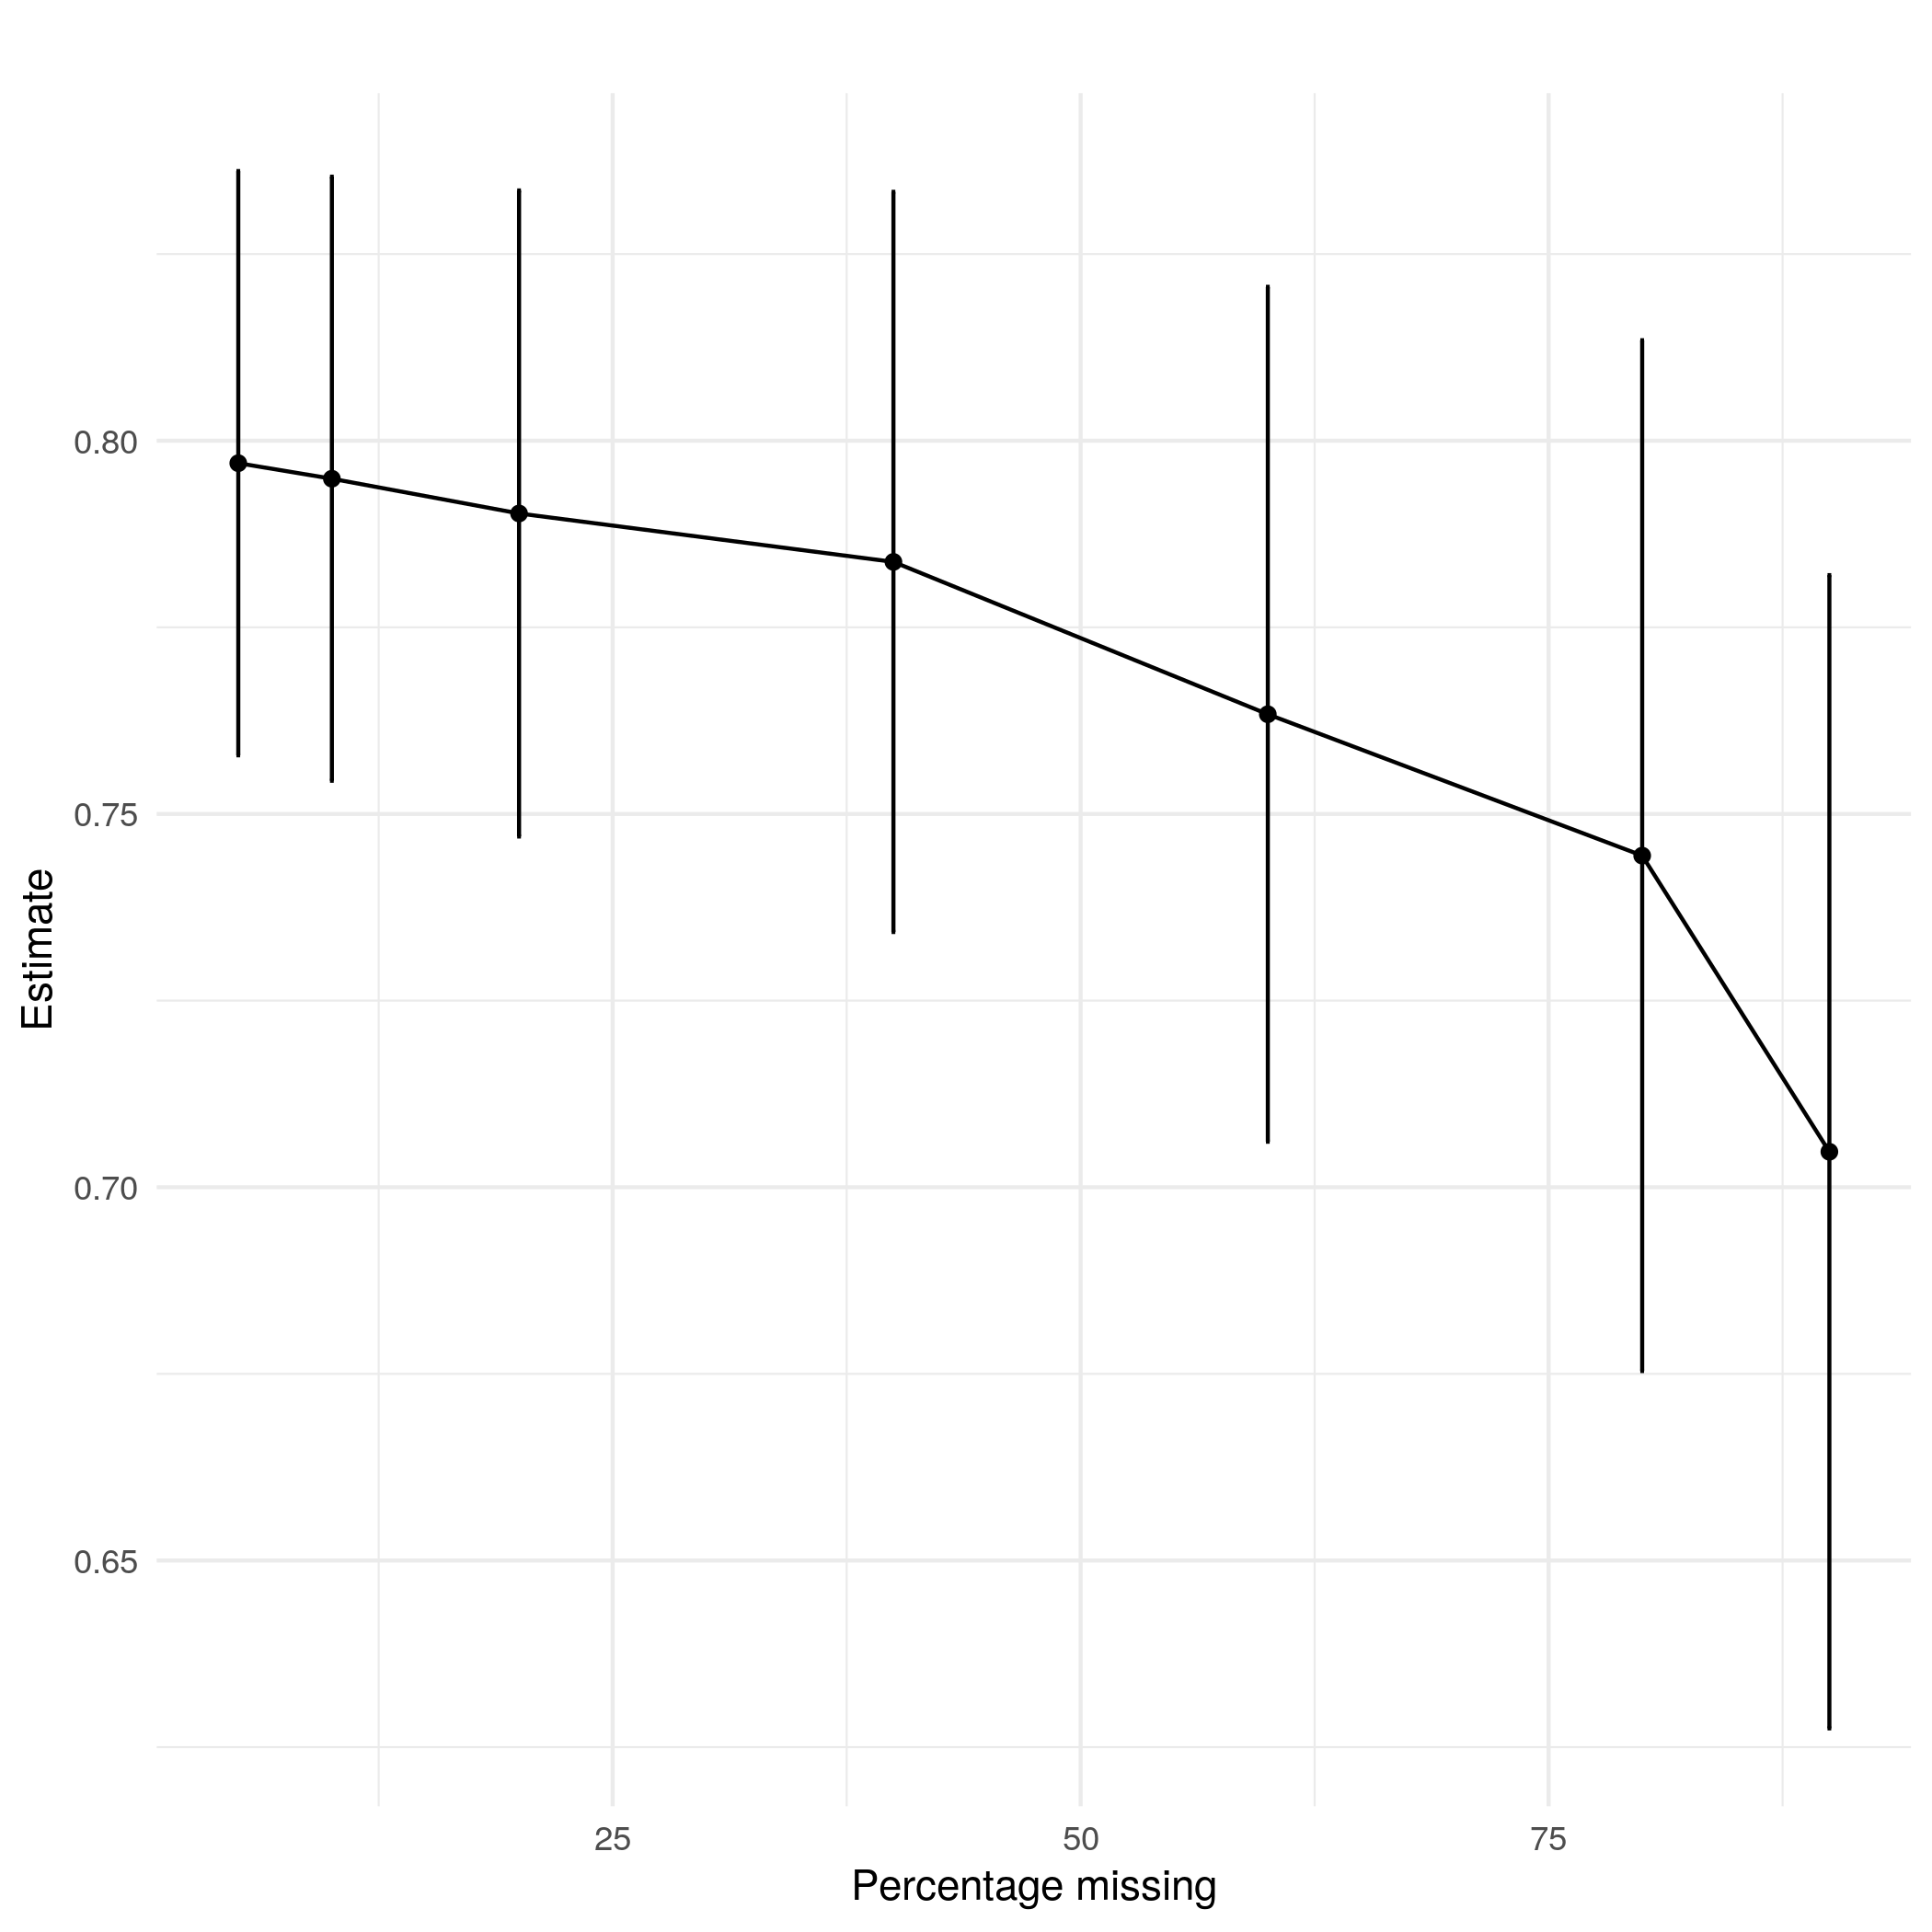
\includegraphics[width=0.3\textwidth]{final_estimate_mi.png}}
	\\
	\subfloat[Coverage]{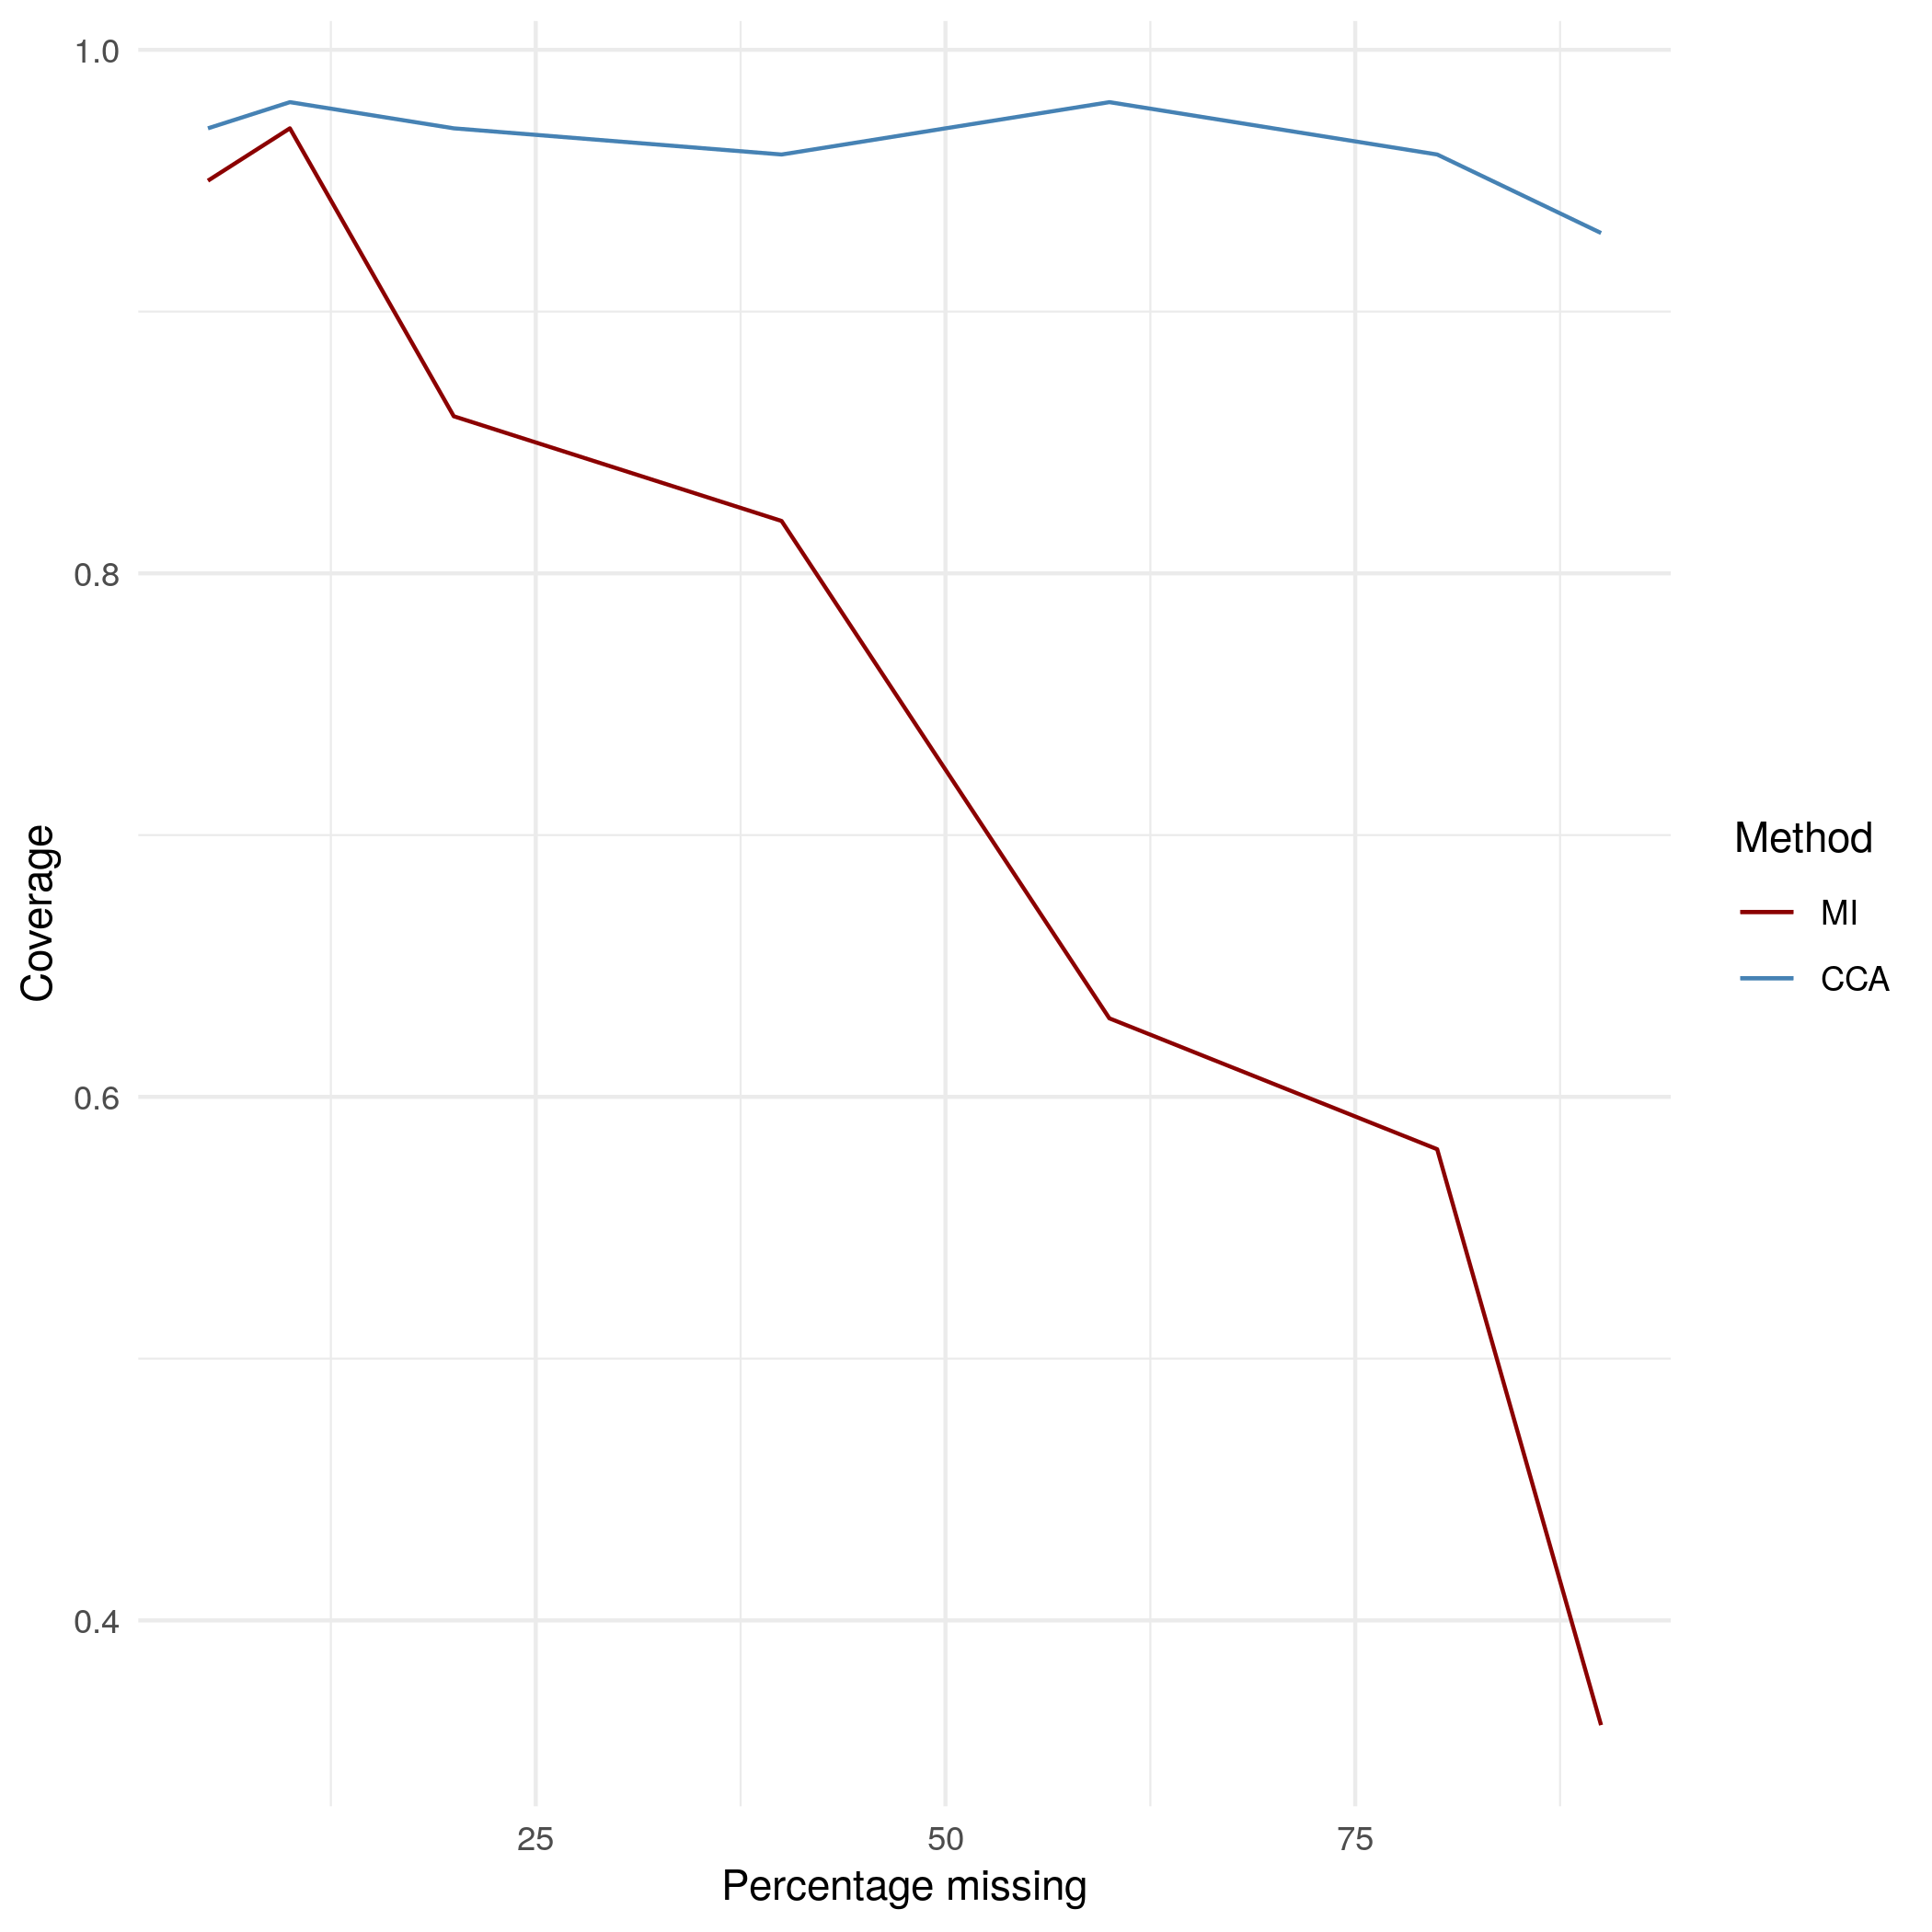
\includegraphics[width=0.2\textwidth]{final_coverage.png}}
	\quad
	\subfloat[Average CI size]{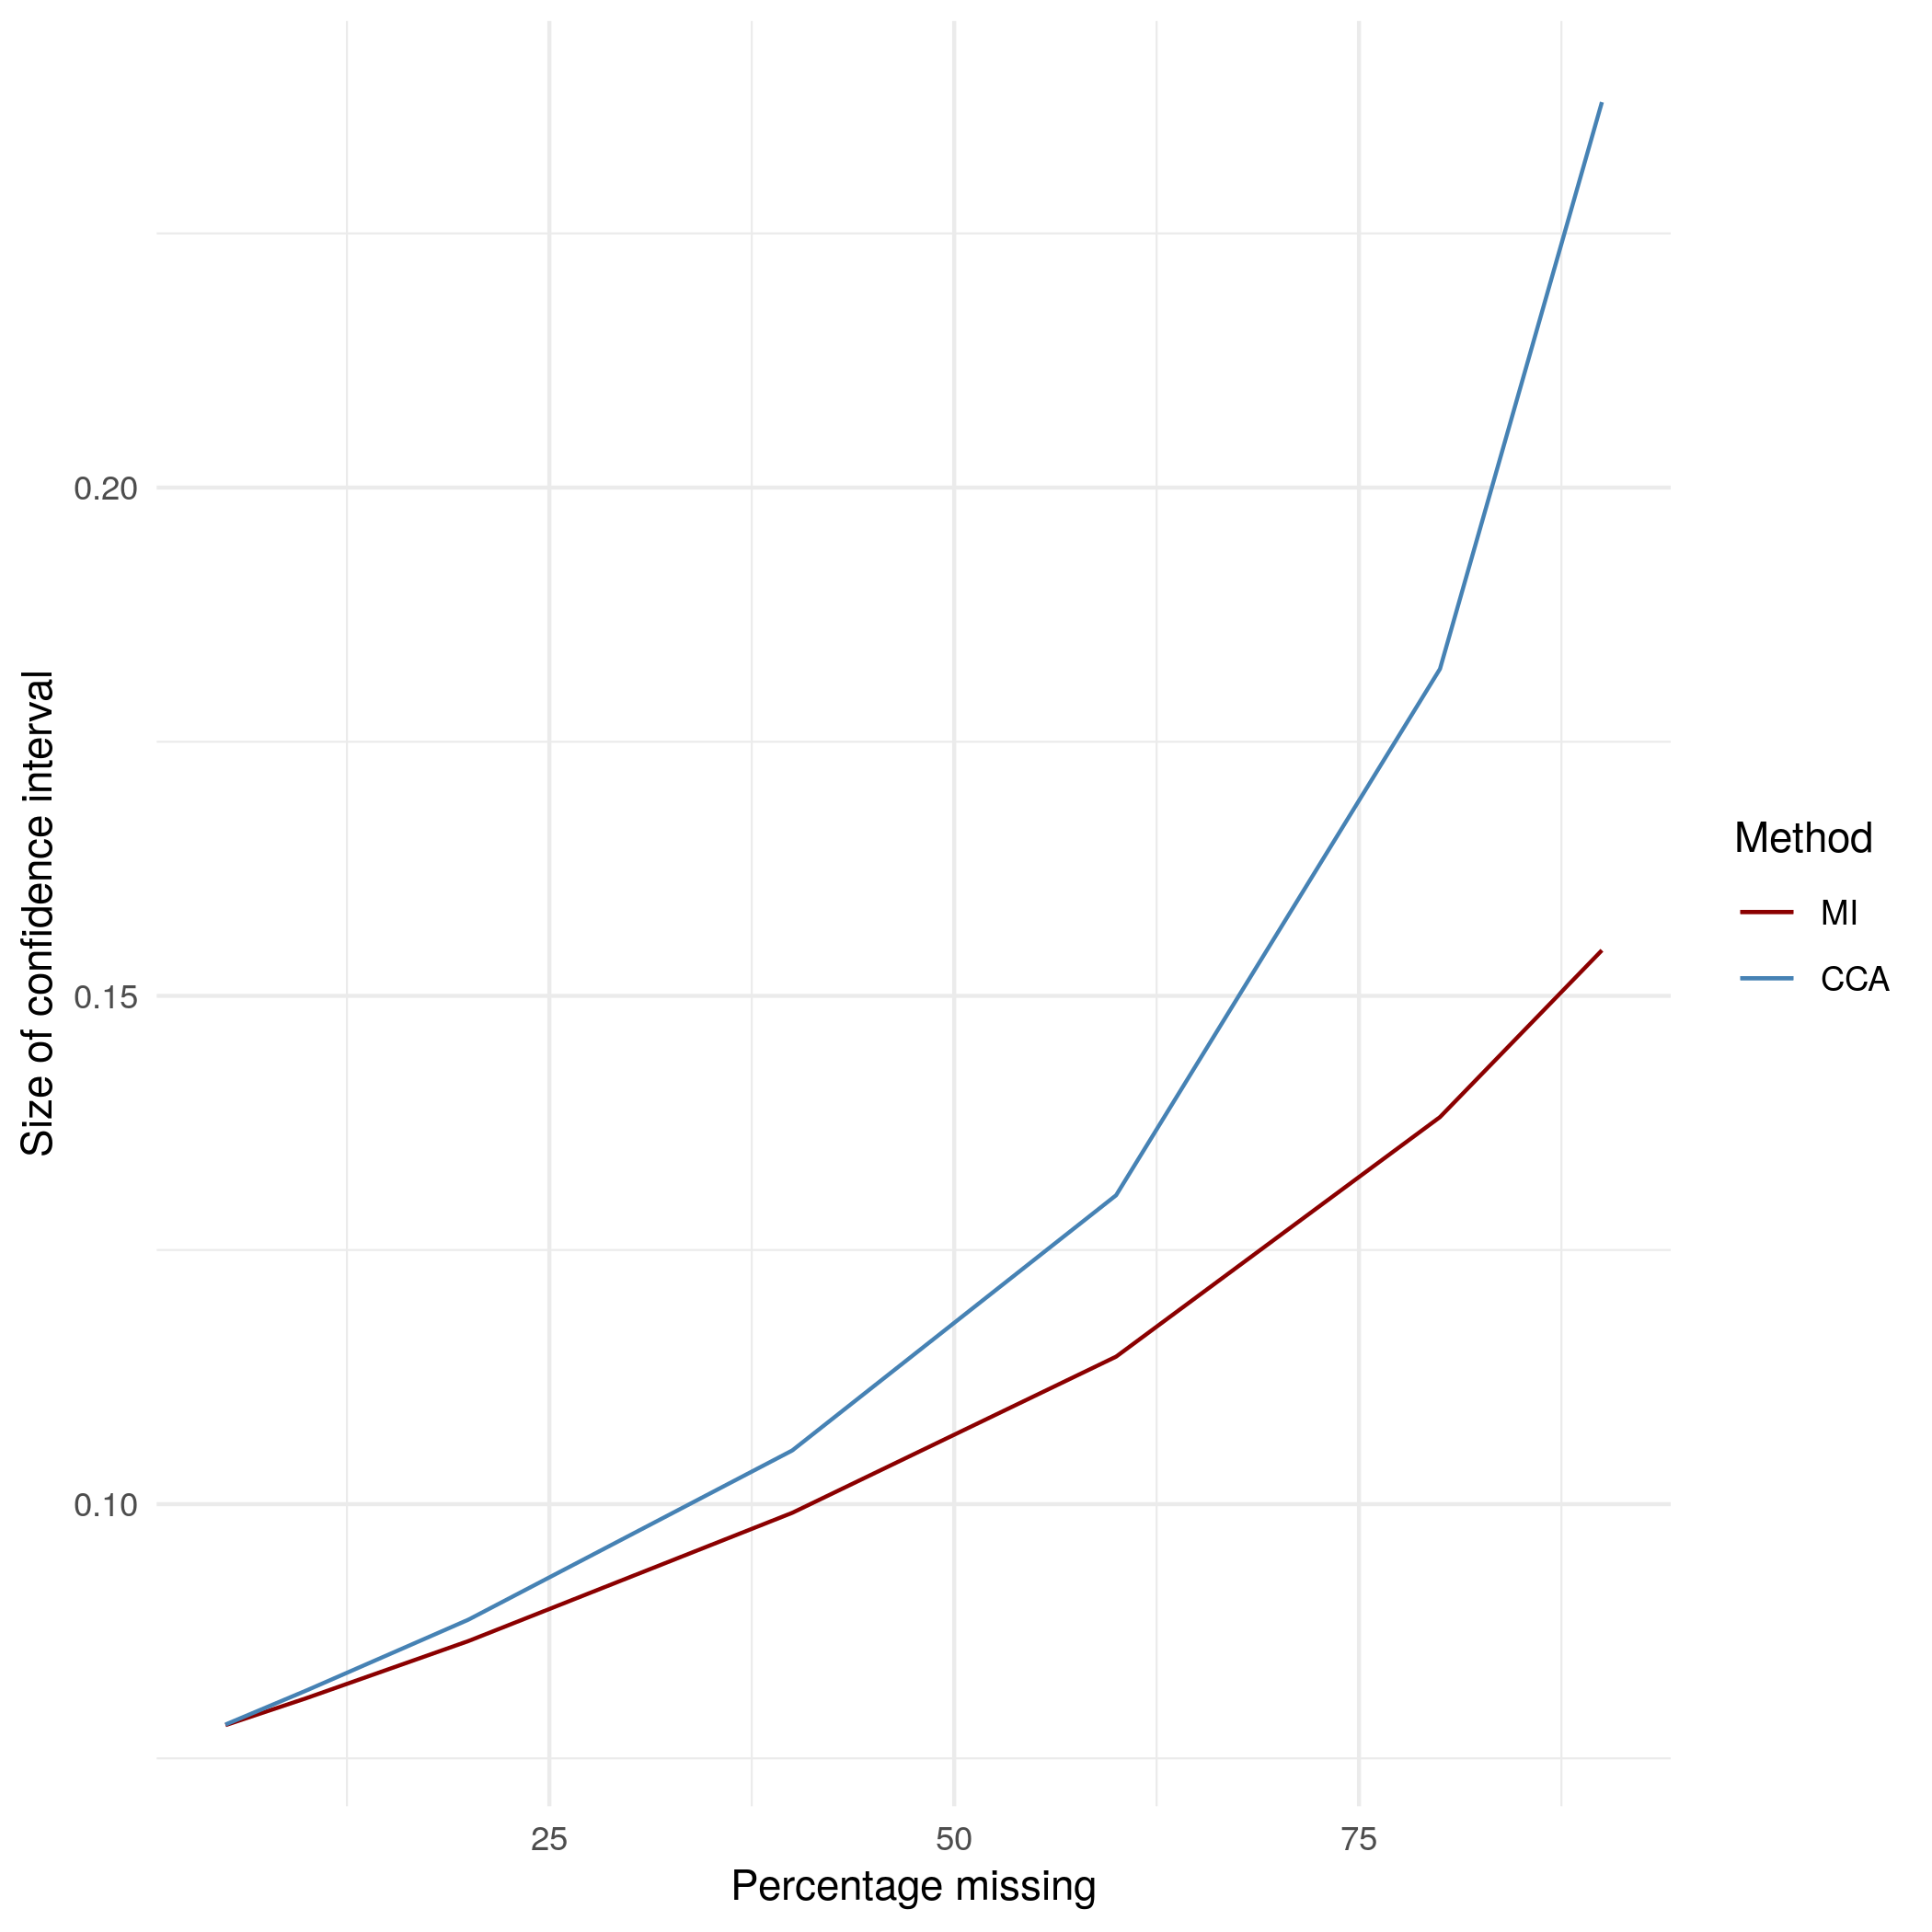
\includegraphics[width=0.2\textwidth]{final_ci.png}}
	\quad
	\subfloat[Average bias]{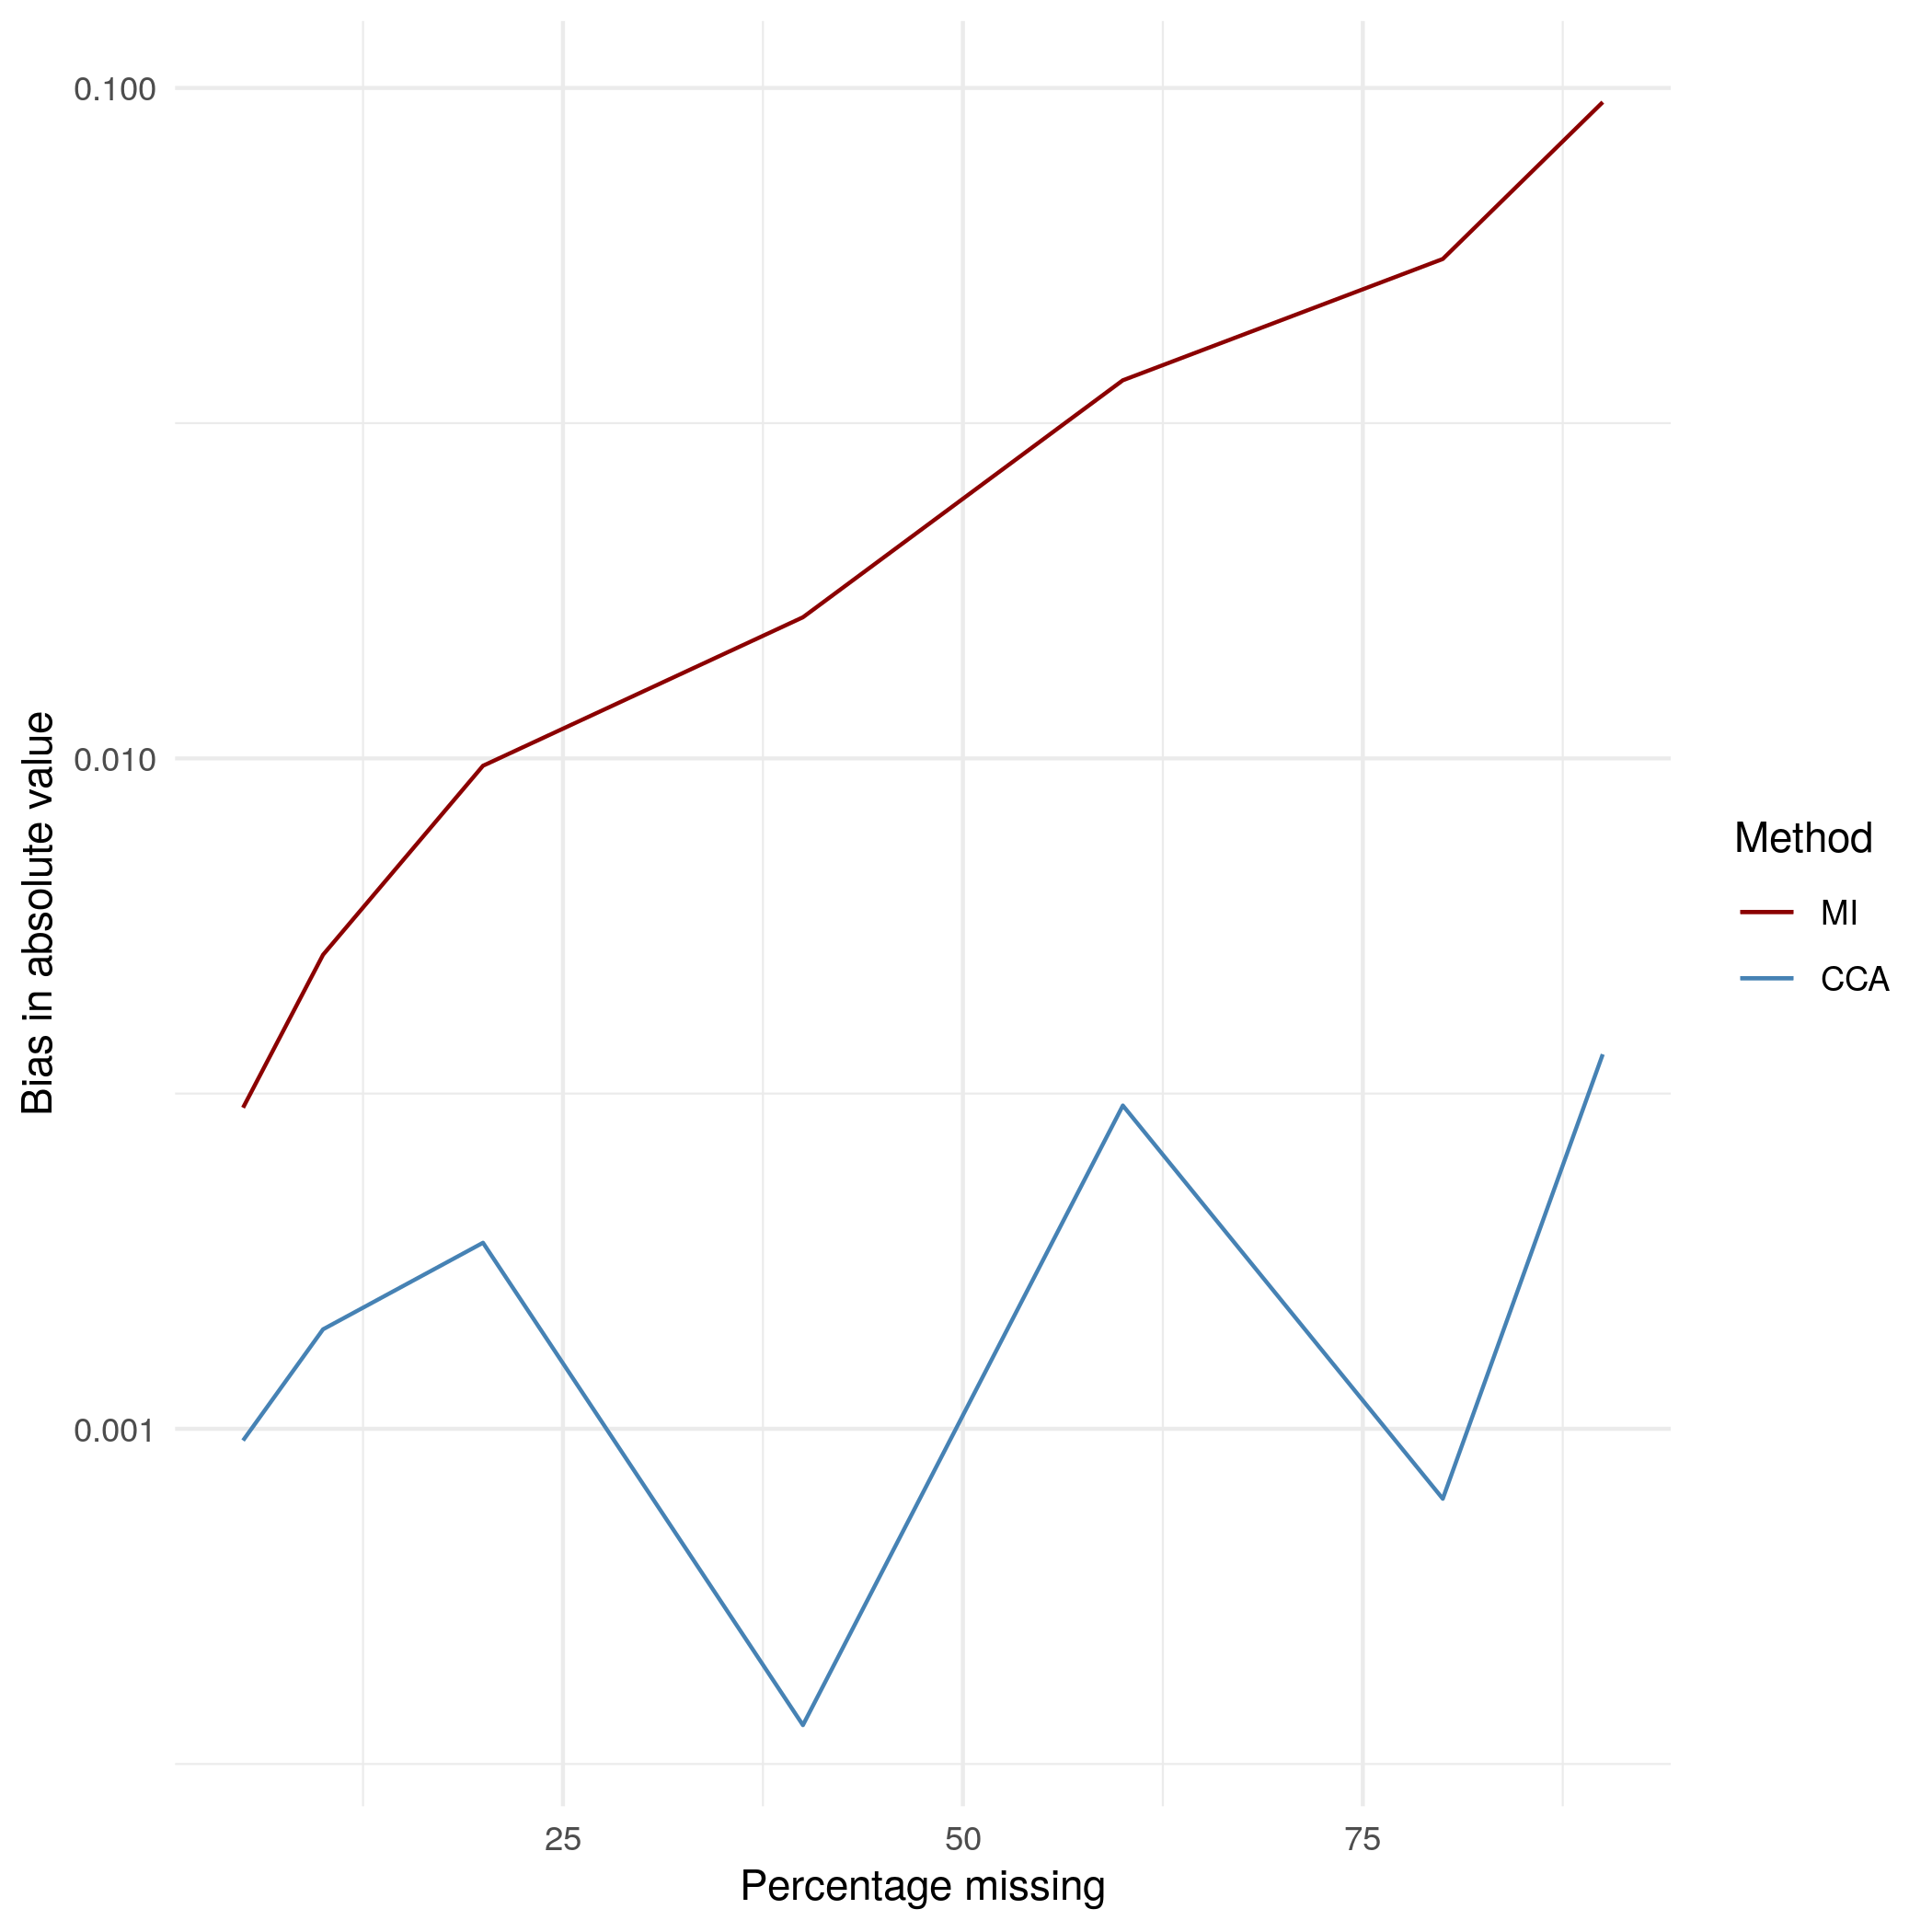
\includegraphics[width=0.2\textwidth]{final_bias.png}}
\end{figure}
\end{frame}

\begin{frame}
\frametitle{MNAR}
\begin{figure}[H]
	\centering
	\subfloat[$\beta_{1}$ estimate with CCA]{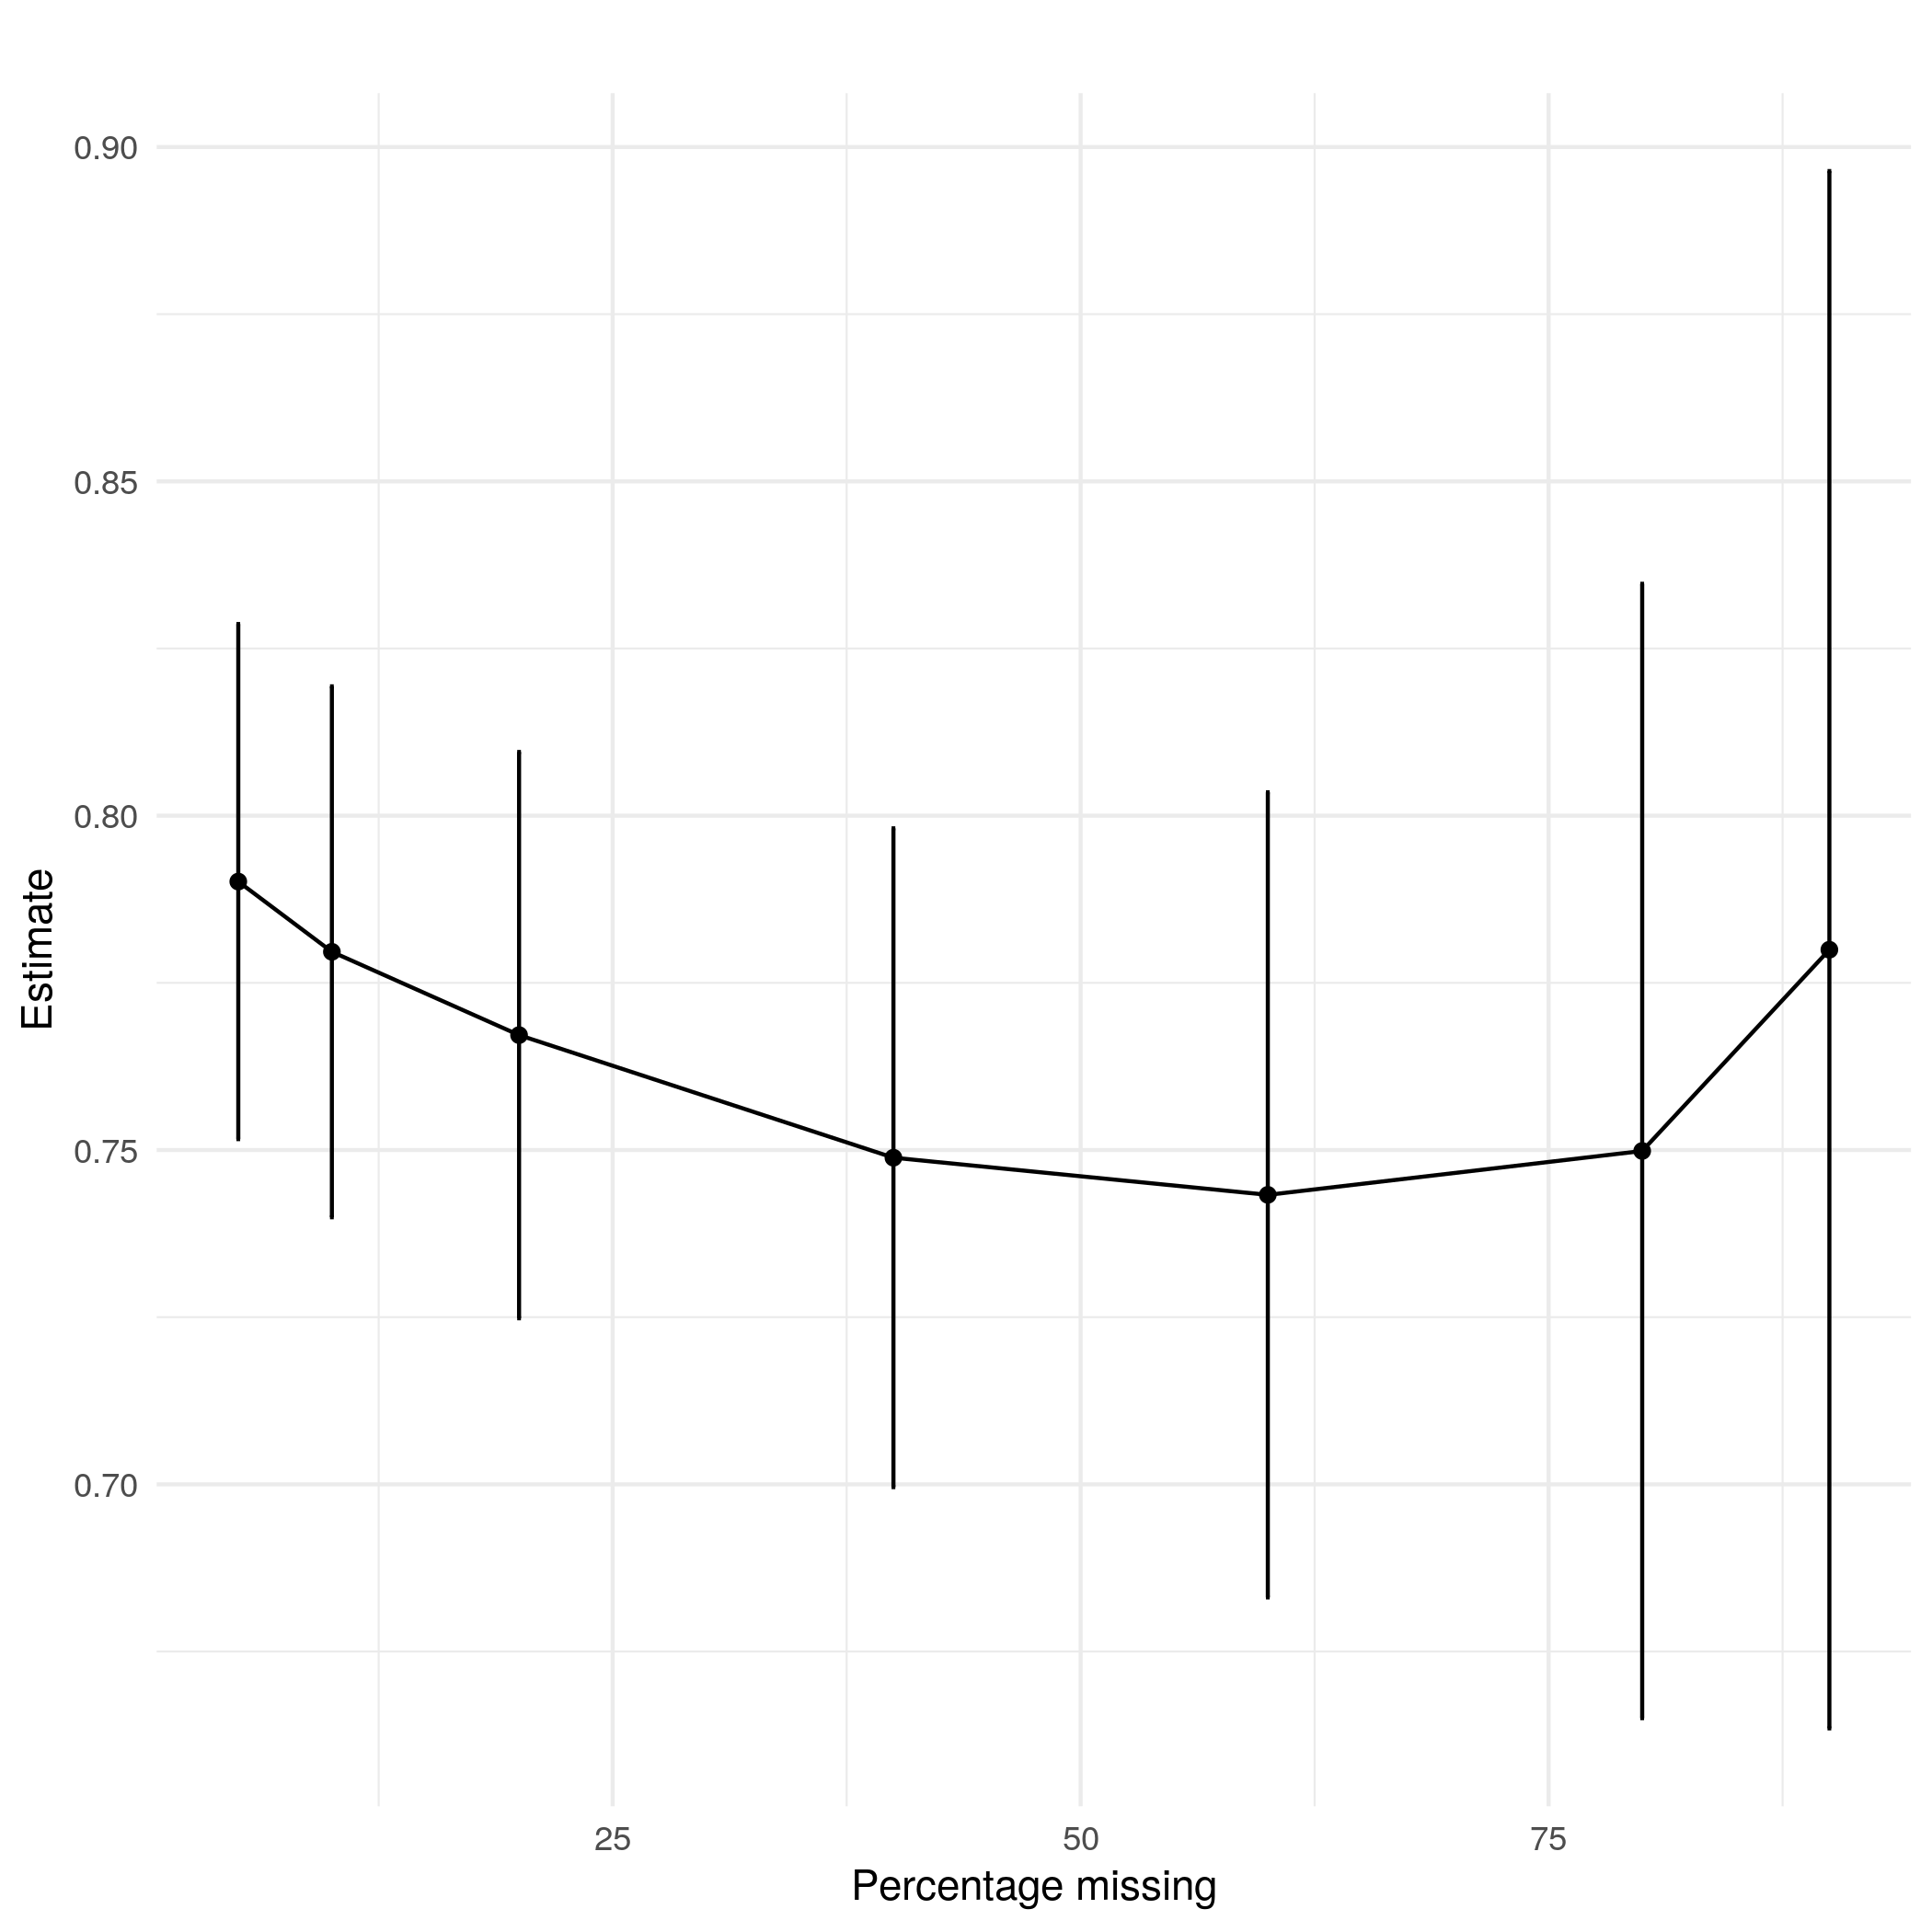
\includegraphics[width=0.3\textwidth]{mnar_final_estimate_cca.png}}
	\quad
	\subfloat[$\beta_{1}$ estimate with MI]{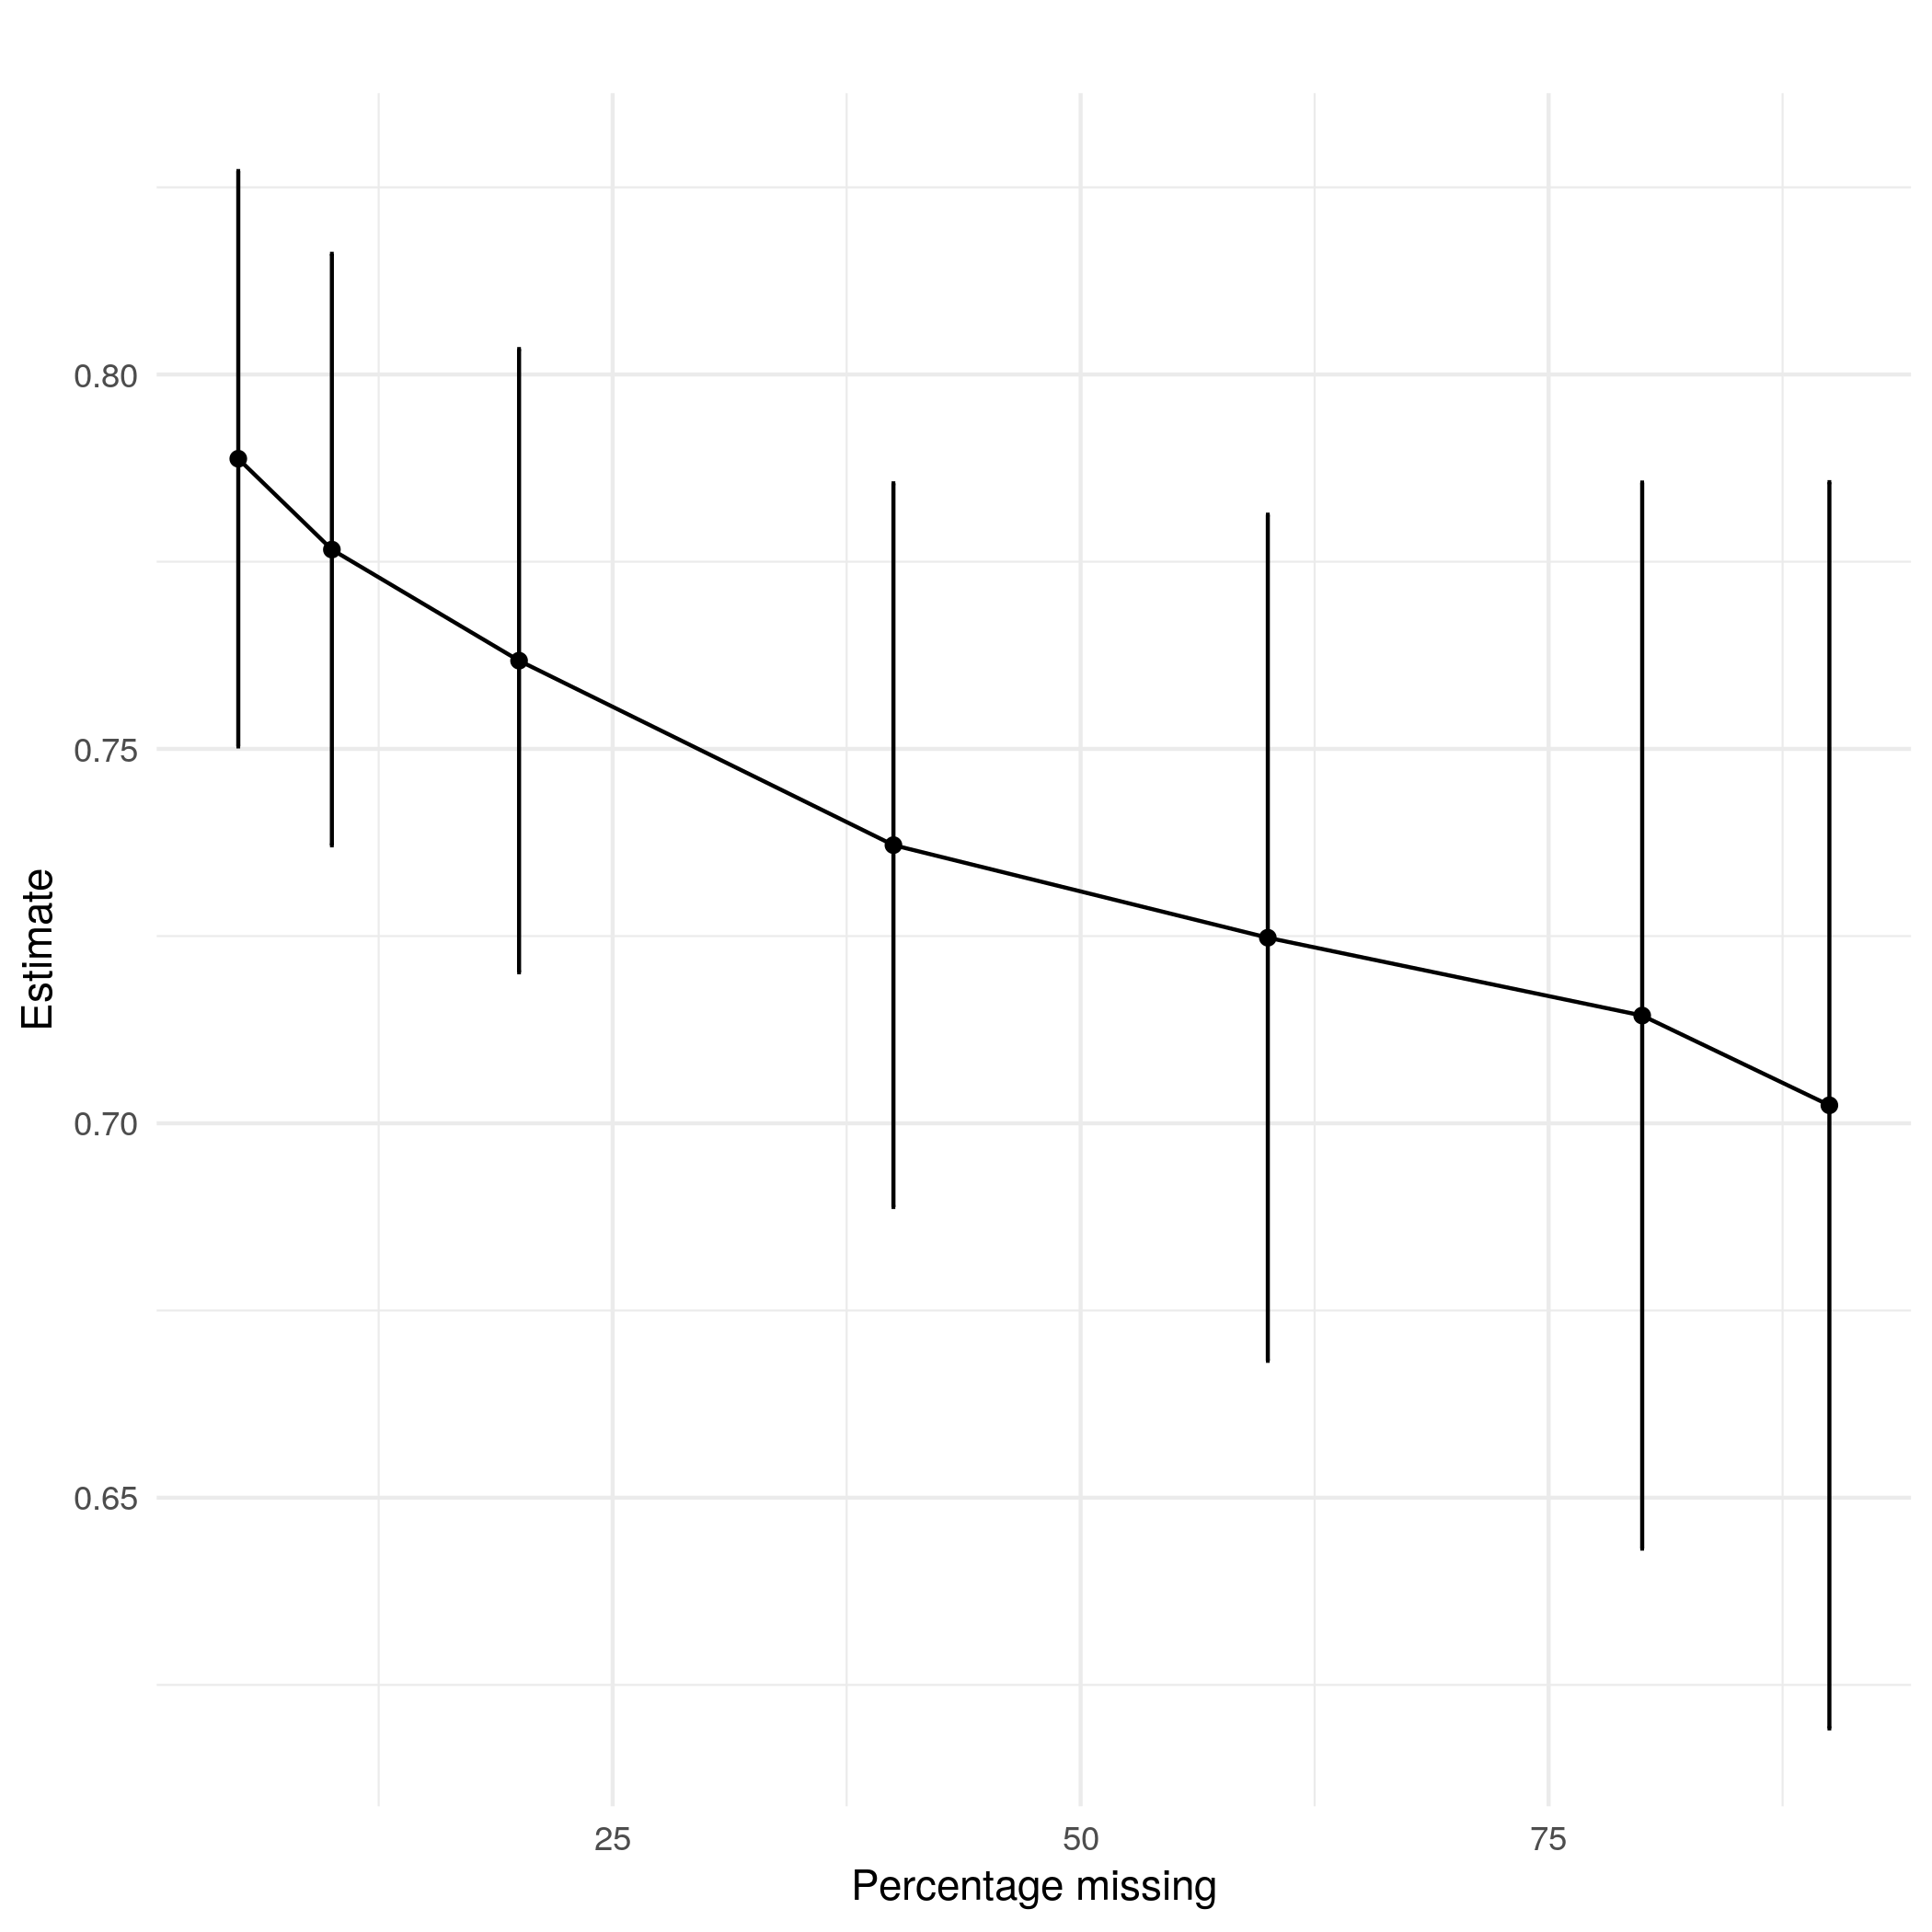
\includegraphics[width=0.3\textwidth]{mnar_final_estimate_mi.png}}
	\\
	\subfloat[Coverage]{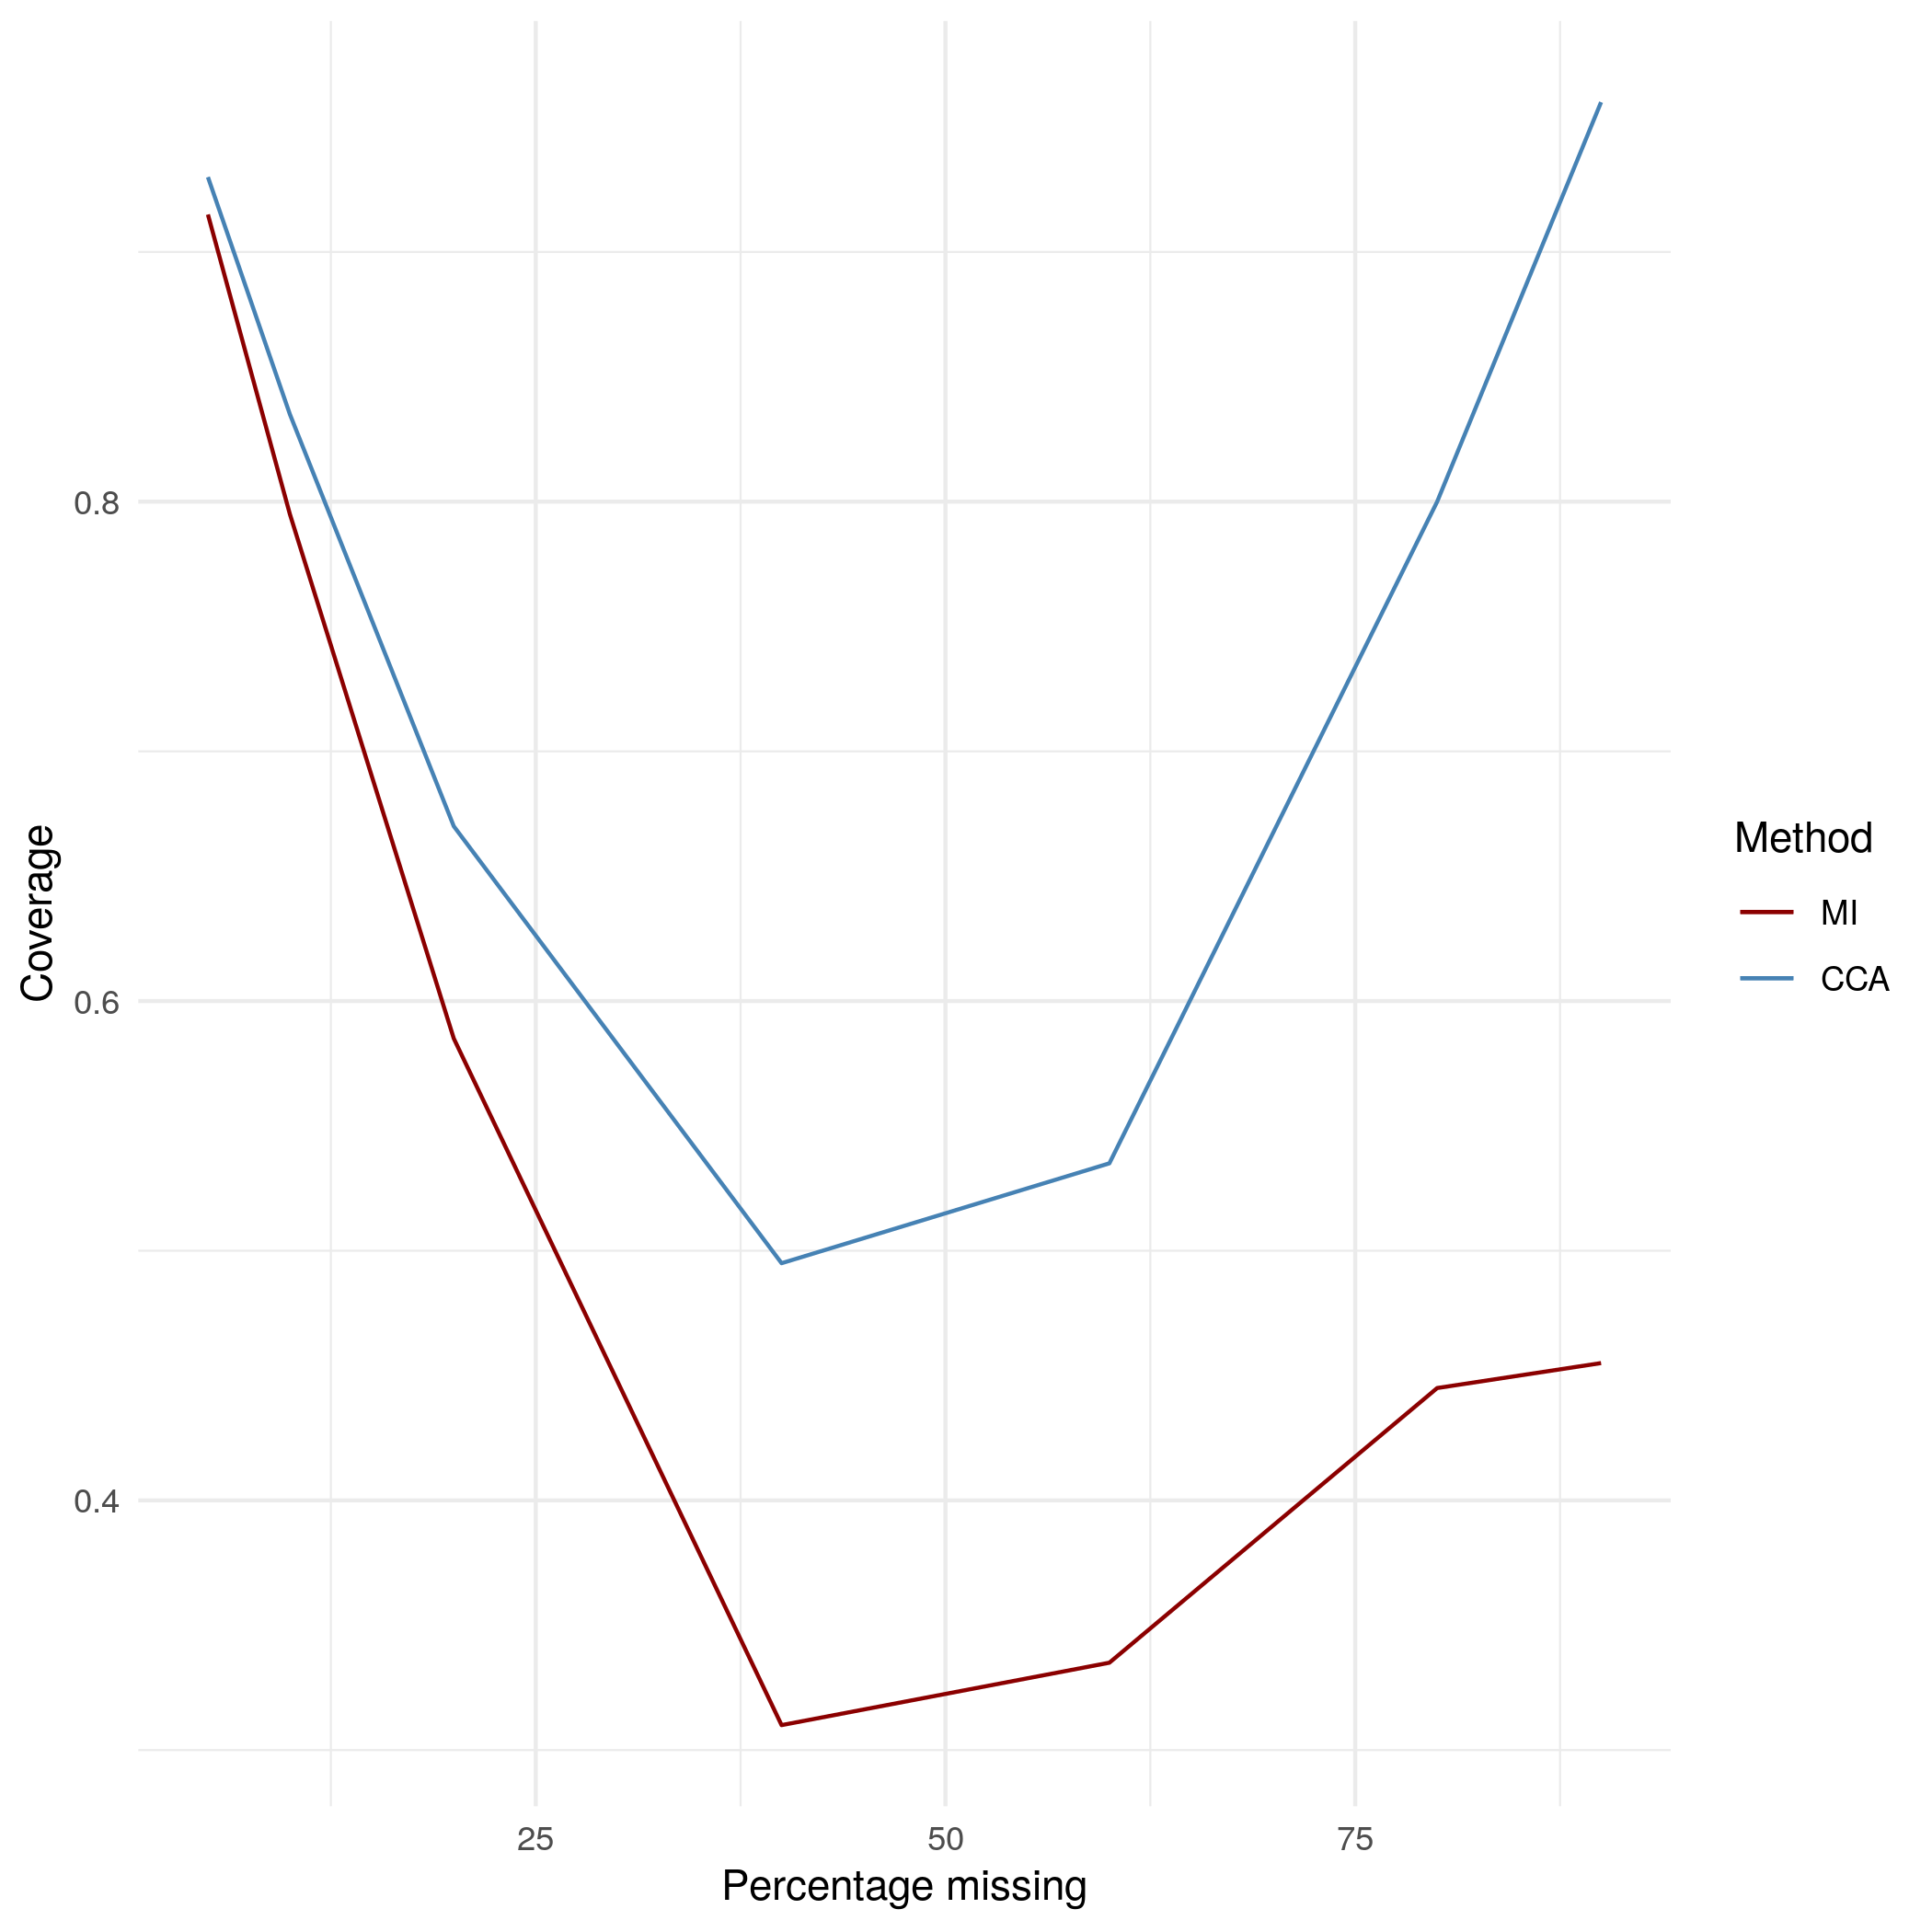
\includegraphics[width=0.2\textwidth]{mnar_final_coverage.png}}
	\quad
	\subfloat[Average CI size]{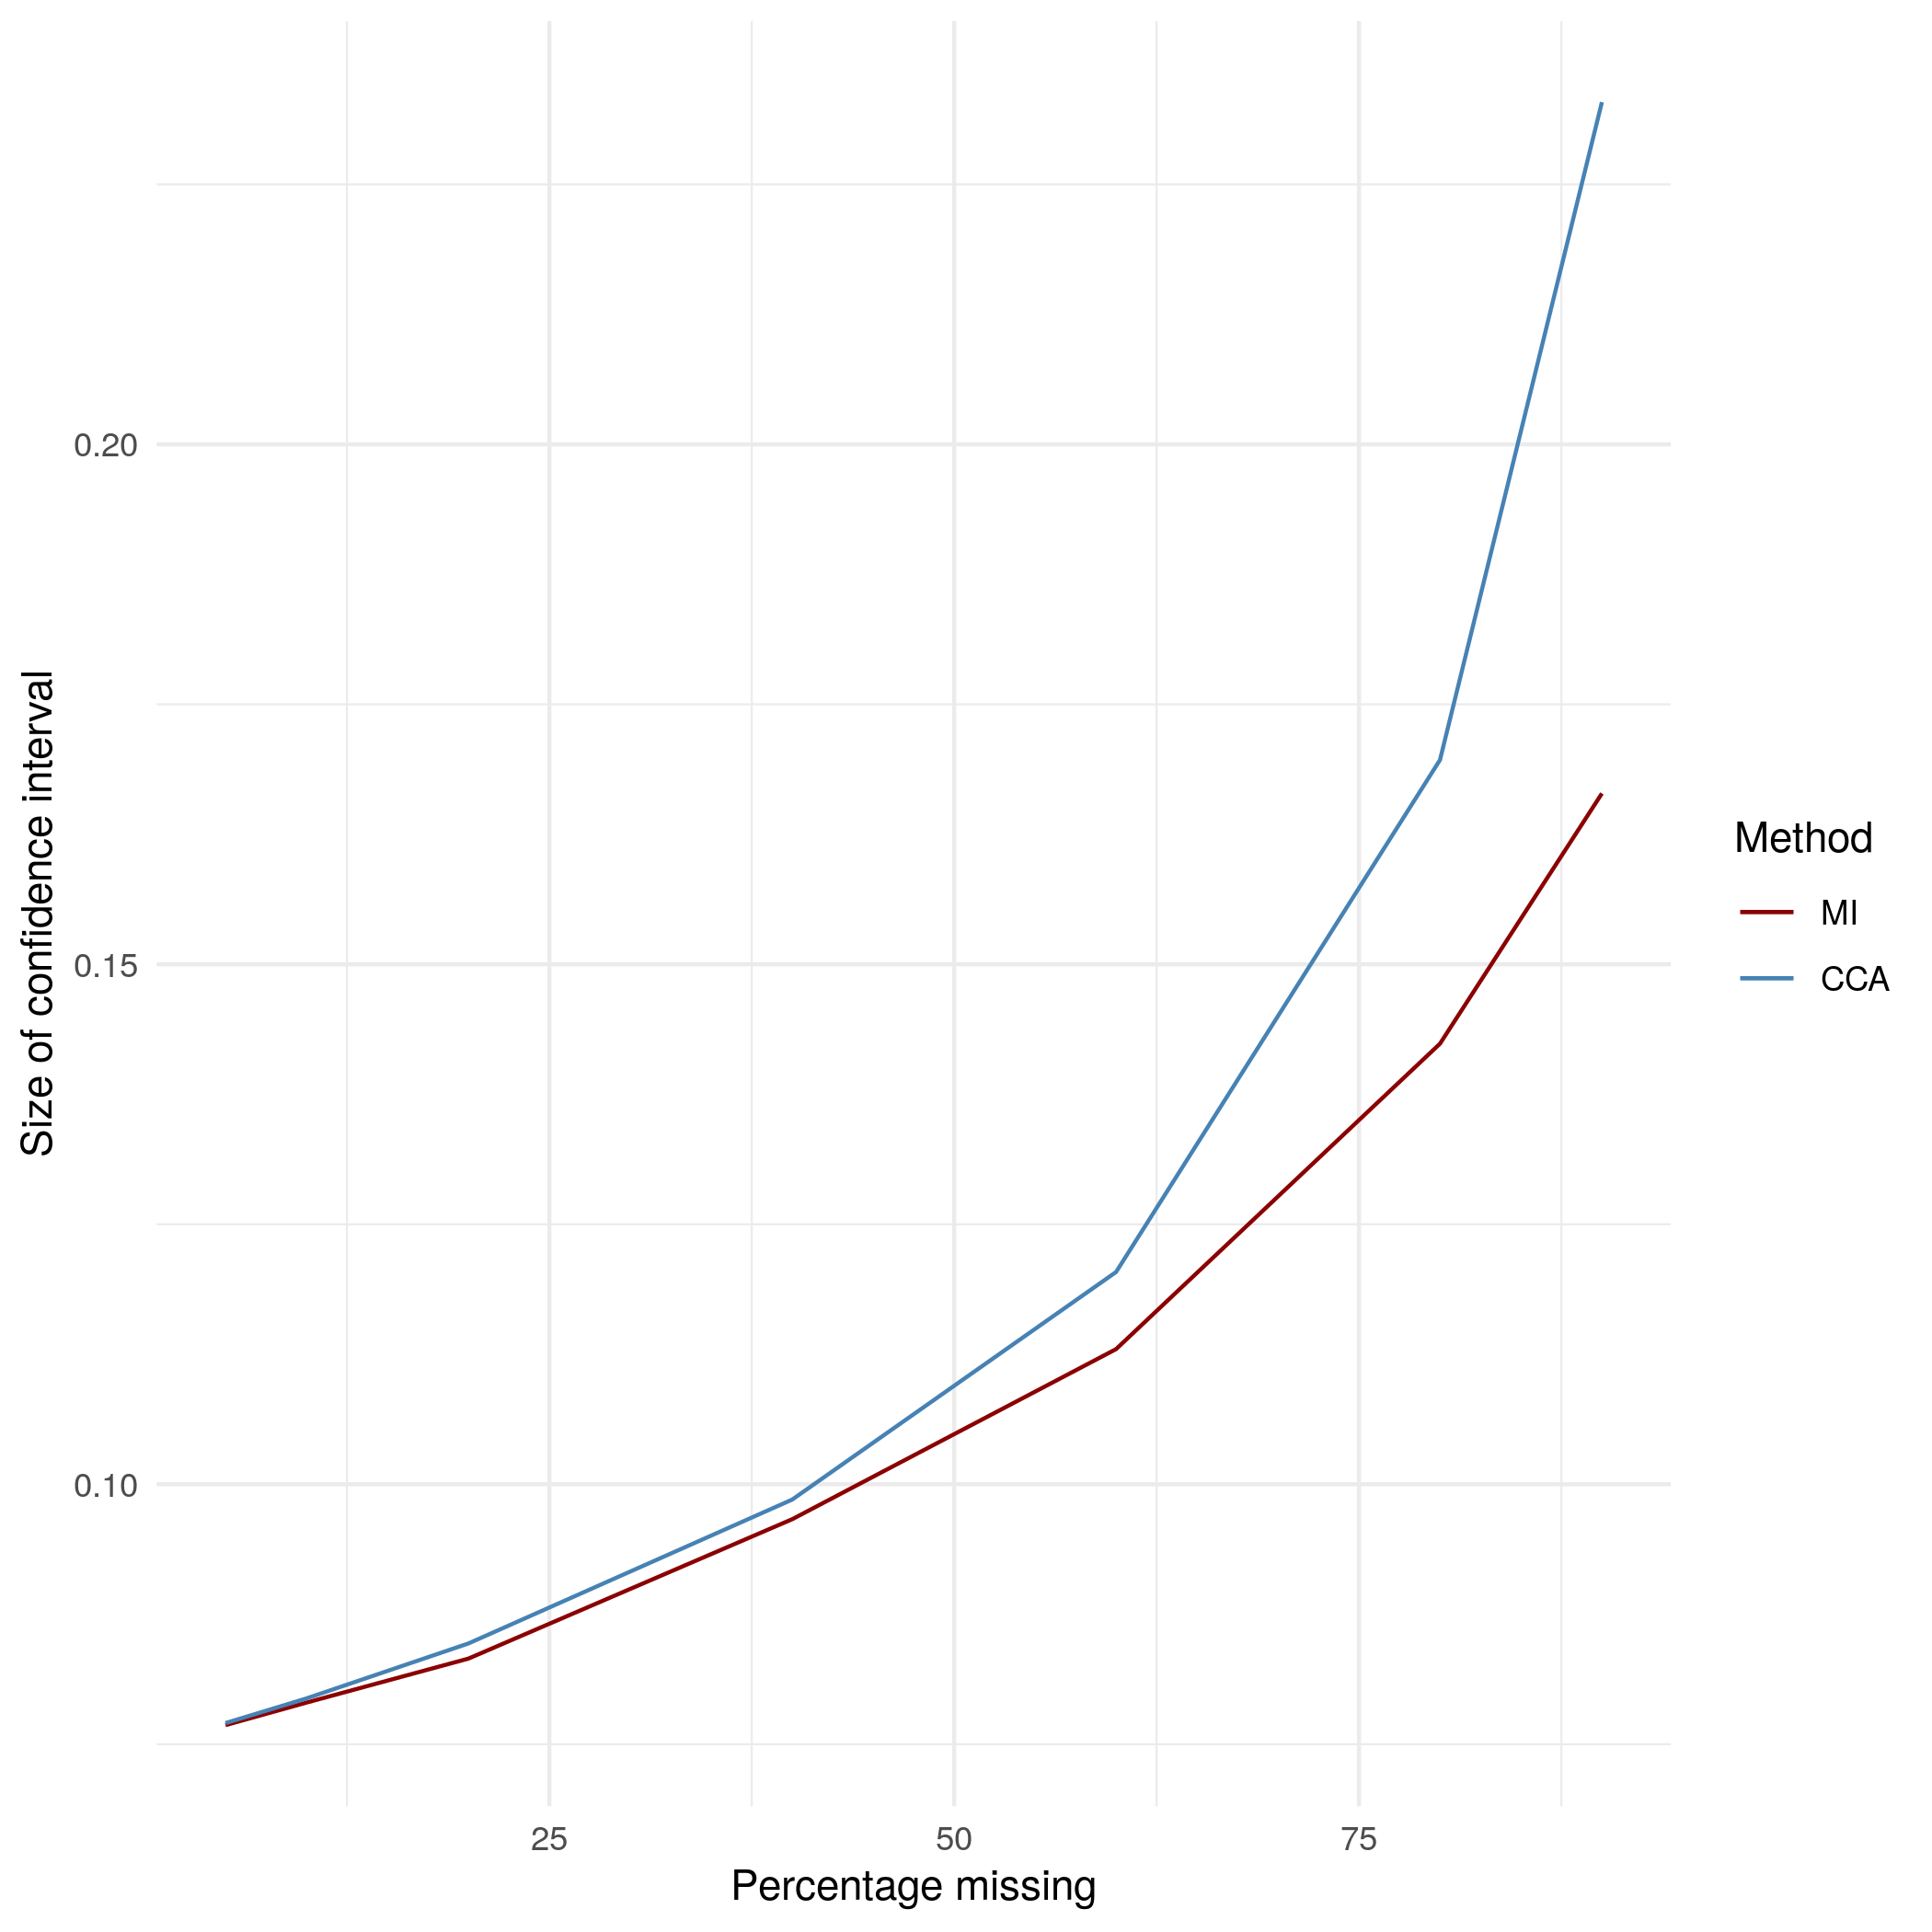
\includegraphics[width=0.2\textwidth]{mnar_final_ci.png}}
	\quad
	\subfloat[Average bias]{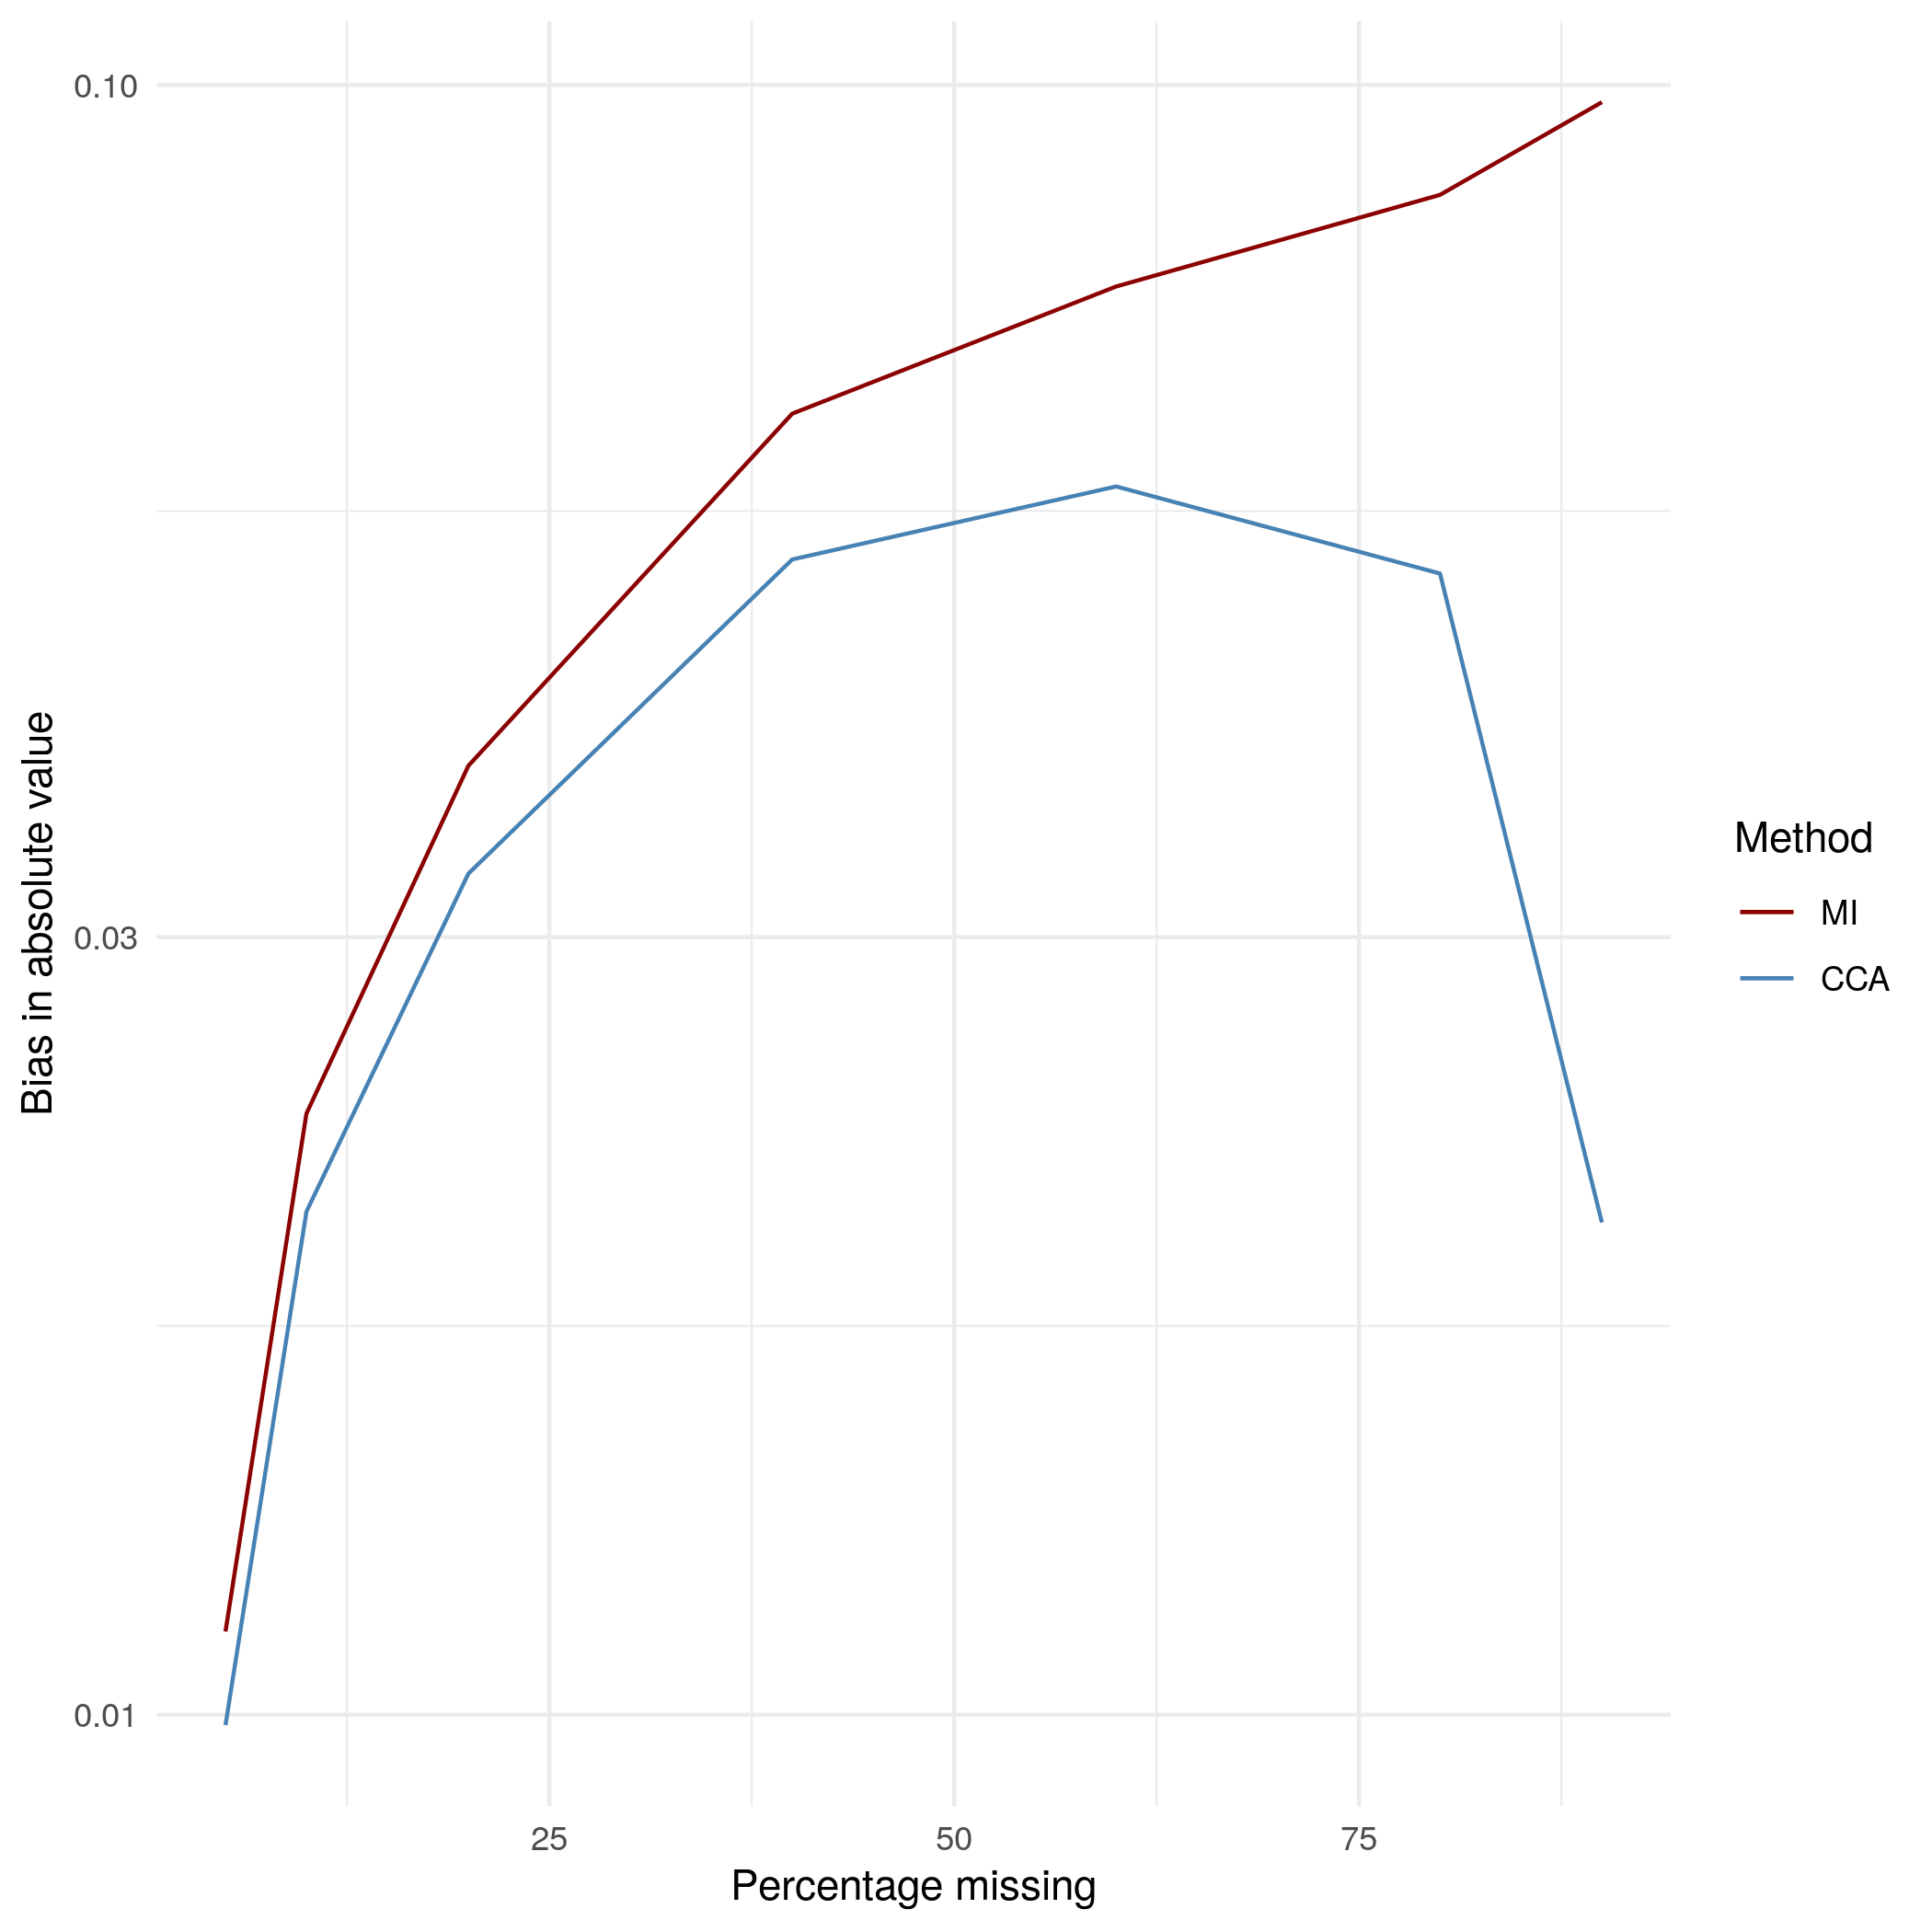
\includegraphics[width=0.2\textwidth]{mnar_final_bias.png}}
\end{figure}
\end{frame}


\section{Conclusion and further work}
\begin{frame}
\frametitle{Conclusion and further work}
We conclude that:
\begin{enumerate}
	\item<1-> Missing data is an important consideration in data analysis.
	\item<2-> Imputation can in certain circumstances help with missing data.
	\item<3-> Theory and literature disagree with experimental results. Further study will be needed to verify these results.
\end{enumerate}
\end{frame}

\begin{frame}
\frametitle{Conclusion and further work}
We conclude that:
\begin{enumerate}
	\item Missing data is an important consideration in data analysis.
	\item Imputation can in certain circumstances help with missing data.
	\item Theory and literature disagree with experimental results. Further study will be needed to verify these results.
\end{enumerate}
Possible future investigations could be made into the effect of MI on prediction and classification, especially in the context of machine learning models. Another interesting avenue of exploration is replacing the conditional distributions with other modeling tools such as trees or neural networks. Perhaps the messy nature of much of modern data will make the underlying assumptions of conditional distributions untenable.
\end{frame}

\bibliography{final_5_bib}	
\bibliographystyle{apalike}
\end{document}
